\documentclass[11pt]{article}

\usepackage[margin=1in]{geometry}
\usepackage{fontspec}
\usepackage{amsmath,amssymb,amsthm,mathtools}
\usepackage{booktabs,array,longtable,multirow}
\usepackage{enumitem}
\usepackage{graphicx}
\usepackage{caption}
\usepackage{subcaption}
\usepackage{float}
\usepackage{xcolor}
\usepackage{microtype}
\usepackage{hyperref}
\usepackage[nameinlink,noabbrev]{cleveref}

\graphicspath{{./}{./toricgt_pg_softmoe_figures/}{./toricgt_extended_figures/}}
\IfFontExistsTF{Noto Serif Hebrew}
  {\newfontfamily\hebrewfont{Noto Serif Hebrew}}
  {\newfontfamily\hebrewfont{Arial Unicode MS}}
\newcommand{\heb}[1]{{\hebrewfont #1}}

\hypersetup{
  colorlinks=true,
  linkcolor=blue!55!black,
  citecolor=blue!55!black,
  urlcolor=blue!55!black
}

\theoremstyle{definition}
\newtheorem{definition}{Definition}[section]
\newtheorem{assumption}[definition]{Assumption}
\newtheorem{example}[definition]{Example}
\theoremstyle{plain}
\newtheorem{theorem}[definition]{Theorem}
\newtheorem{lemma}[definition]{Lemma}
\newtheorem{proposition}[definition]{Proposition}
\newtheorem{corollary}[definition]{Corollary}
\theoremstyle{remark}
\newtheorem{remark}[definition]{Remark}

\numberwithin{equation}{section}

\newcommand{\R}{\mathbb{R}}
\newcommand{\C}{\mathbb{C}}
\newcommand{\Z}{\mathbb{Z}}
\newcommand{\Q}{\mathbb{Q}}
\newcommand{\N}{\mathbb{N}}
\newcommand{\T}{\mathbb{T}}
\newcommand{\one}{\mathbf{1}}
\newcommand{\A}{\mathcal{A}}
\newcommand{\G}{\mathcal{G}}
\newcommand{\V}{\mathcal{V}}
\newcommand{\E}{\mathcal{E}}
\newcommand{\X}{\mathcal{X}}
\newcommand{\Y}{\mathcal{Y}}
\newcommand{\F}{\mathcal{F}}
\newcommand{\Tok}{\mathsf{Tok}}
\newcommand{\Graph}{\mathsf{Graph}}
\newcommand{\Phase}{\mathsf{Phase}}
\newcommand{\Root}{\mathsf{Root}}
\newcommand{\Pat}{\mathsf{Pat}}
\newcommand{\Binyan}{\mathsf{Binyan}}
\newcommand{\Feat}{\mathsf{Feat}}
\newcommand{\softmax}{\operatorname{softmax}}
\newcommand{\diag}{\operatorname{diag}}
\newcommand{\argmax}{\operatorname*{arg\,max}}
\newcommand{\argmin}{\operatorname*{arg\,min}}
\newcommand{\supp}{\operatorname{supp}}
\newcommand{\Tr}{\operatorname{Tr}}
\newcommand{\rank}{\operatorname{rank}}
\newcommand{\Var}{\operatorname{Var}}
\newcommand{\Eop}{\mathbb{E}}
\newcommand{\dist}{\operatorname{dist}}
\newcommand{\poly}{\operatorname{poly}}
\newcommand{\Conv}{\operatorname{Conv}}
\newcommand{\Newt}{\operatorname{Newt}}
\newcommand{\ReLU}{\operatorname{ReLU}}
\newcommand{\Fan}{\operatorname{Fan}}
\newcommand{\Vol}{\operatorname{Vol}}
\newcommand{\norm}[1]{\left\lVert #1\right\rVert}
\newcommand{\abs}[1]{\left\lvert #1\right\rvert}
\newcommand{\ip}[2]{\left\langle #1,#2\right\rangle}
\newcommand{\transpose}{^{\mathsf T}}
\newcommand{\defeq}{\vcentcolon=}
\newcommand{\OO}{\mathcal O}
\newcommand{\HH}{\mathcal H}
\newcommand{\Ext}{\operatorname{Ext}}
\newcommand{\Tor}{\operatorname{Tor}}
\newcommand{\Hom}{\operatorname{Hom}}
\newcommand{\End}{\operatorname{End}}
\newcommand{\Spec}{\operatorname{Spec}}
\newcommand{\im}{\operatorname{im}}
\newcommand{\coker}{\operatorname{coker}}
\newcommand{\gr}{\operatorname{gr}}

\title{\vspace{-2em}ToricGT with Toric BGG Supervision: Graph-Token Reasoning, Hypertoric Category $\mathcal O$, and BPB-Constrained Training}
\author{Amelie Schreiber}
\date{June 2026}

\begin{document}
\maketitle


\begin{abstract}
ToricGT is a graph-token Transformer framework for algebraic and graph-structured reasoning under stringent compression and evaluation constraints.  The paper makes the toric component operational rather than decorative.  We introduce a Toric BGG training layer built from finite shadows of hypertoric category $\mathcal O$, oriented-matroid category $\mathcal O$, multigraded BGG correspondences, toric Tate resolutions, and Euler-Koszul complexes.  These objects supply small, verifiable certificates for reasoning trajectories: sign-vector posets, standard filtrations, sparse differentials, Betti profiles, Gale-dual labels, active faces of Newton polytopes, and homological consistency checks.  The certificates are attached through low-rank probes to the existing ToricGT stack: TokenGT-style node/edge tokenization, tropical ring attention, noncommutative torus phase channels, Soft-MoE routing, GraphCG concept axes, embedding-space GFlowNet search, and trajectory-retrieval memory.  For the Parameter-Golf branch we add a byte-scored TokenGT hybrid: official BPB remains a byte-level prequential log score, while FineWeb byte paths and graph-of-thought examples receive causal or noncausal TokenGT-style graph losses on hidden reveal trajectories.  We prove equivariance and stability statements for graph-token layers, tropical active faces, Soft-MoE dispatch, prefix-causal byte scoring, BGG differentials, incidence-algebra proxies, chain-map supervision, Gale-dual curricula, BPB-safe interpolation heads, and behavior-corridor projections.  We also develop behavior-modification protocols that generalize Assistant-Axis capping into GraphCG-disentangled toric-tropical corridors and alcoves, with Stanley--Reisner, toric-ideal, Fitting, free-resolution, and DG-algebra barriers for graph-of-thought trajectories, memory, and analogy.  The methodology is designed for implementation: certificates are cached on CPU, GPU losses have small rank and sparse support, activation gates are staged, ablations are explicit, and evaluation remains centered on BPB and held-out reasoning quality.  The central design principle is that toric BGG theory should improve training by organizing hidden reasoning into exact finite complexes, while deployable models retain only the components that improve validation BPB, graph-reasoning accuracy, retrieval quality, behavior reliability, or out-of-distribution algebraic generalization under an auditable artifact budget.
\end{abstract}


\tableofcontents
\newpage


\section{Purpose and high-level architecture}

ToricGT begins from a simple modeling decision: represent structured reasoning problems as typed graphs, tokenize their nodes and edges, and process the resulting token table with a Transformer that respects graph relabeling.  The architecture then adds algebraic structure where the task calls for it.  Tropical heads implement max-plus and min-plus recurrences; ring evaluation changes the memory schedule without changing the exact attention function; noncommutative-torus channels provide projective phase memory; Soft-MoE blocks route typed graph tokens to specialized differentiable computations; GraphCG-style coordinates make concept directions inspectable; and GFlowNet fine-tuning samples diverse graph-of-thought completions.

The contribution of this revision is the Toric BGG layer.  The term is used in a precise but finite sense.  Hypertoric category $\mathcal O$ and category $\mathcal O$ for quantized conical symplectic resolutions give a toric analogue of BGG representation theory: highest-weight structure, standard and costandard objects, Koszulity, and Gale-dual behavior.  Multigraded BGG and toric Tate resolutions give a computational companion in toric commutative algebra.  ToricGT uses these theories to build small certificates that can be attached to training examples: a finite poset of chambers or sign vectors, a sparse chain complex, standard-filtration masks, a Betti table or Koszul degree profile, a Gale-dual partner, and optional Euler-Koszul data.  The model is trained not only to predict the answer, but to produce hidden trajectories whose local moves behave like differentials and whose analogical transfers behave like approximate exact functors between finite complexes.

The architecture is therefore separated into three levels of claim.  At the first level are exact statements about finite graph-token computations: tokenization, masking, attention, decoding, Soft-MoE routing, tropical ring evaluation, prefix-causal byte scoring, and BGG certificate losses are equivariant or score-valid under explicitly stated hypotheses.  At the second level are approximation statements on bounded graph families and bounded certificate families.  At the third level are empirical hypotheses: Toric BGG certificates should improve generalization on algebraic reasoning, retrieval, and graph-of-thought tasks, and should improve or at least not damage BPB when distilled into a byte-constrained language model.  Those hypotheses are evaluated by ablations rather than asserted as theory.

\paragraph{Model family.}
A ToricGT instance consists of
\begin{equation}
  \mathsf{ToricGT}=D\circ \Phi_L\circ\cdots\circ\Phi_1\circ T,
\end{equation}
where $T$ is a graph tokenizer, each $\Phi_\ell$ is a token-permutation-equivariant block with softmax, tropical, hybrid, or ring-evaluated attention, and $D$ is a shared node/edge/graph decoder.  Optional side modules supply toric phase transports, BGG certificate probes, GraphCG coordinate heads, GFlowNet policies, trajectory-memory retrieval, and long-context cache compression.  In a BPB-constrained deployment, most of these probes are training-only; they survive in the final artifact only if they improve the held-out log score under the byte budget.

\begin{figure}[p]
  \centering
  \includegraphics[width=\textwidth]{toricgt_architecture_and_training_diagram.png}
  \caption{ToricGT architecture and training program.  Typed graph tokens carry node, edge, endpoint, structural, tropical, toric phase, and optional BGG-certificate features.  The encoder combines ordinary attention, tropical ring attention, Soft-MoE adapters, and low-rank certificate probes.  Training combines supervised graph losses, BPB or language-model loss, GFlowNet trajectory balance, GraphCG disentanglement, and Toric BGG homological consistency.}
  \label{fig:architecture}
\end{figure}

\paragraph{Core invariants.}
The model is engineered around six invariants.
\begin{enumerate}[leftmargin=2em]
  \item \emph{Graph-to-graph equivariance}: relabeling a graph relabels node and edge outputs in the same way.
  \item \emph{Schedule/function separation}: ring attention changes the evaluation schedule, not the mathematical attention function being evaluated.
  \item \emph{Semiring visibility}: tropical heads expose active maximizers and margins, so dynamic-programming decisions can be inspected.
  \item \emph{Projective algebraic memory}: toric phase channels encode twisted commutation and cocycles without claiming that a finite network represents an infinite $C^*$-algebra.
  \item \emph{Homological discipline}: when a training record carries a Toric BGG certificate, the hidden trajectory is asked to satisfy finite chain-complex, standard-filtration, Koszul, or Gale-dual constraints.
  \item \emph{BPB accountability}: auxiliary structure is retained in compressed language-model deployments only when it improves score-before-update validation BPB or a predeclared reasoning metric without leakage.
\end{enumerate}
\section{Typed attributed graph domains}

\subsection{Graph objects}

\begin{definition}[Typed attributed directed multigraph]
A typed attributed graph is a tuple
\begin{equation}
  G=(V,E,s,t,\tau_V,\tau_E,x,e,m_V,m_E),
\end{equation}
where $V=\{1,\ldots,n\}$ is a finite vertex set, $E=\{1,\ldots,m\}$ is a finite edge-token set, $s,t:E\to V$ are source and target maps, $\tau_V:V\to\mathcal T_V$ and $\tau_E:E\to\mathcal T_E$ are finite type maps, $x_i\in\R^{d_v}$ and $e_a\in\R^{d_e}$ are bounded real attributes, and $m_V,m_E$ are masks when the graph is embedded into a padded domain.
\end{definition}

The edge set is treated as a set of edge tokens rather than as raw file-order rows.  This matters: file order is rarely a graph invariant.  For a node relabeling $\pi\in S_n$, an edge $a$ with endpoints $(s(a),t(a))$ is transformed to an edge with endpoints $(\pi s(a),\pi t(a))$.  If edge tokens are stored by a canonical endpoint order, this induces an edge permutation $\rho_\pi$; if edge tokens are stored unordered, $\rho_\pi$ is any consistent action on the edge-token set.

\begin{definition}[Padded bounded graph cell]
Fix $N_{\max}$ and $M_{\max}$.  A padded graph cell $\G_{n,m,I,\tau}$ consists of graphs with exactly $n\le N_{\max}$ valid nodes, $m\le M_{\max}$ valid edges, fixed endpoint pattern $I\in\{1,\ldots,n\}^{m\times 2}$, fixed node and edge type pattern $\tau$, and attributes in compact sets $K_V\subset\R^{d_v}$ and $K_E\subset\R^{d_e}$.  The full bounded domain is the finite union
\begin{equation}
  \G_{\le N,\le M}=\bigcup_{n\le N,\,m\le M,\,I,\tau}\G_{n,m,I,\tau}.
\end{equation}
\end{definition}

\begin{lemma}[Compactness of cells]
Every graph cell $\G_{n,m,I,\tau}$ is compact.  The bounded padded graph space $\G_{\le N,\le M}$ is a finite union of compact cells and is therefore compact when equipped with the disjoint-union topology or with a mask topology that separates cells.
\end{lemma}

\begin{proof}
Fix $n,m,I,\tau$.  The only continuous degrees of freedom are node attributes $X\in K_V^n$ and edge attributes $E\in K_E^m$.  Finite products of compact sets are compact by Tychonoff's theorem in the finite case, equivalently by Heine-Borel when the sets are closed and bounded subsets of Euclidean space.  Endpoint and type data are fixed discrete parameters in the cell.  Hence $\G_{n,m,I,\tau}\simeq K_V^n\times K_E^m$ is compact.  There are finitely many masks, endpoint patterns, and type patterns under fixed $N$ and $M$, so the union is finite.  A finite union of compact sets is compact.
\end{proof}

\begin{lemma}[Induced edge permutations form an action]
Suppose edge canonicalization is label-compatible: for all $\pi,\sigma\in S_n$, canonicalizing after $\sigma$ and then after $\pi$ is the same as canonicalizing after $\pi\sigma$.  Then $\rho_{\pi\sigma}=\rho_\pi\rho_\sigma$ and $\rho_{\mathrm{id}}=\mathrm{id}$.
\end{lemma}

\begin{proof}
Let $a$ be an edge token with endpoints $(u,v)$.  Applying $\sigma$ sends the endpoints to $(\sigma u,\sigma v)$ and moves the token to position $\rho_\sigma(a)$.  Applying $\pi$ next sends endpoints to $(\pi\sigma u,\pi\sigma v)$ and token position to $\rho_\pi(\rho_\sigma(a))$.  Direct application of $\pi\sigma$ gives the same endpoint pair.  By label-compatible canonicalization the same edge-token position is assigned, so $\rho_{\pi\sigma}(a)=\rho_\pi\rho_\sigma(a)$ for every $a$.  The identity relabeling leaves endpoints and canonical order unchanged.
\end{proof}

\begin{definition}[Graph-to-graph equivariance]
Let $P_\pi=\pi\oplus\rho_\pi$ be the induced token permutation on node and edge outputs.  A graph-to-graph map $F:\G\to\Y_V^n\times\Y_E^m\times\Y_G$ is equivariant if
\begin{equation}
  F(\pi\cdot G)=\bigl(P_\pi F_{V,E}(G),F_G(G)\bigr)
\end{equation}
for every admissible relabeling $\pi$.  Its graph-level component is invariant when $F_G(\pi\cdot G)=F_G(G)$.
\end{definition}

\section{Tokenization as an equivariant construction}

\subsection{Token maps}

A graph tokenizer maps typed attributed graphs to token matrices.  Node and edge tokens have distinct type channels, endpoint channels, structural identifiers, and optional toric phase channels.  For a node $i$ and an edge token $a=(u,v)$,
\begin{align}
  t_i^V &= \phi_V(x_i,\tau_V(i)) + \eta_i + \kappa_i + \theta_i,\\
  t_a^E &= \phi_E(e_a,\tau_E(a)) + \psi(\eta_u,\eta_v) + \zeta_a + \kappa_a + \theta_a.
\end{align}
Here $\eta_i$ is an equivariant node identifier, $\zeta_a$ is an edge identifier, $\kappa$ denotes optional structural features such as degree or Laplacian information, and $\theta$ denotes optional toric phase features.  The maps $\phi_V,\phi_E,\psi$ are shared across all nodes and edges.

\begin{assumption}[Equivariant identifiers]
The identifier fields obey
\begin{equation}
  \eta_i(\pi G)=\eta_{\pi^{-1}i}(G),\qquad
  \zeta_a(\pi G)=\zeta_{\rho_\pi^{-1}a}(G),
\end{equation}
and structural/phase channels obey the analogous transformation law.
\end{assumption}

\begin{lemma}[Tokenization equivariance]
Under equivariant identifiers and shared endpoint maps,
\begin{equation}
  T(\pi\cdot G)=P_\pi T(G).
\end{equation}
\end{lemma}

\begin{proof}
For a node token,
\begin{align}
  t_i^V(\pi G)
  &=\phi_V(x_{\pi^{-1}i},\tau_V(\pi^{-1}i))+\eta_{\pi^{-1}i}+\kappa_{\pi^{-1}i}+\theta_{\pi^{-1}i}\\
  &=(P_\pi T(G))_i.
\end{align}
For an edge token $a$ in the relabeled graph, its preimage under $\rho_\pi$ is $\rho_\pi^{-1}a$.  Its source and target identifiers are the permuted identifiers of the original endpoints.  Since $\phi_E$ and $\psi$ are shared, the edge token after relabeling equals the edge token at $\rho_\pi^{-1}a$ before relabeling.  Concatenating node and edge rows gives $P_\pi T(G)$.
\end{proof}

\begin{lemma}[Mask equivariance]
Let $M(G)\in\{0,-\infty\}^{L\times L}$ be an additive attention mask whose entries depend only on token validity, token types, and graph incidence relations.  Then
\begin{equation}
  M(\pi G)=P_\pi M(G)P_\pi\transpose.
\end{equation}
\end{lemma}

\begin{proof}
Validity masks permute with valid token rows.  Type masks are preserved because node tokens map to node tokens and edge tokens map to edge tokens.  Incidence masks are preserved because $a$ is incident to $i$ exactly when $\rho_\pi a$ is incident to $\pi i$.  Thus every masked or unmasked pair is carried to its relabeled pair, which is exactly conjugation by $P_\pi$.
\end{proof}

\subsection{Attention and block equivariance}

For token matrix $Z\in\R^{L\times d}$, define
\begin{equation}
  Q=ZW_Q,\\quad K=ZW_K,
  \quad V=ZW_V,
  \quad S=QK\transpose/\sqrt{d_h}.
\end{equation}
A softmax head computes $\softmax(S+M)V$.  A max-plus tropical head computes
\begin{equation}
  Y_{ic}=\max_j\{S_{ij}+M_{ij}+V_{jc}\}.
\end{equation}

\begin{lemma}[Softmax and tropical attention are token equivariant]
For any token permutation matrix $P$ and mask satisfying $M(PZ)=PM(Z)P\transpose$,
\begin{equation}
  \operatorname{Attn}(PZ)=P\operatorname{Attn}(Z)
\end{equation}
for softmax attention and for tropical attention.
\end{lemma}

\begin{proof}
Linear projections commute with row permutations: $Q(PZ)=PQ(Z)$ and similarly for $K,V$.  Hence the score matrix becomes
\begin{equation}
  S(PZ)=PQK\transpose P\transpose/\sqrt{d_h}=PS(Z)P\transpose.
\end{equation}
For softmax, row-wise exponentiation and normalization are invariant under simultaneous row and column reindexing:
\begin{equation}
  \softmax(PSP\transpose+PMP\transpose)=P\softmax(S+M)P\transpose.
\end{equation}
Multiplication by $PV$ then yields $P\softmax(S+M)V$.  For tropical attention, fix output row $i$ and coordinate $c$.  If $p$ is the permutation represented by $P$, then
\begin{align}
  Y'_{ic}
  &=\max_j\{(PSP\transpose+PMP\transpose)_{ij}+(PV)_{jc}\}\\
  &=\max_j\{S_{p^{-1}i,p^{-1}j}+M_{p^{-1}i,p^{-1}j}+V_{p^{-1}j,c}\}\\
  &=\max_{j'}\{S_{p^{-1}i,j'}+M_{p^{-1}i,j'}+V_{j'c}\}=Y_{p^{-1}i,c}.
\end{align}
Thus $Y'=PY$.
\end{proof}

\begin{lemma}[Row-wise sublayers are equivariant]
Shared feed-forward networks, residual connections, dropout with shared distribution over rows, and layer normalization applied row-wise commute with token permutations.
\end{lemma}

\begin{proof}
A shared feed-forward network $f$ acts as $(f(Z_1),\ldots,f(Z_L))$.  Permuting rows before or after applying the same $f$ gives the same sequence of rows.  Residual addition is row-wise vector addition.  Layer normalization uses statistics within a row, not across row labels.  Dropout is exactly equivariant when the dropout mask is permuted with rows, and distributionally equivariant when masks are independently sampled from the same row-wise distribution.
\end{proof}

\begin{theorem}[TokenGT stack equivariance]
A ToricGT encoder built from equivariant tokenization, equivariant masks, shared attention projections, shared row-wise feed-forward layers, residuals, layer normalization, and shared node/edge decoders is graph-to-graph equivariant.
\end{theorem}

\begin{proof}
Tokenization maps $G$ to $Z$ and $\pi G$ to $P_\pi Z$.  Each encoder block maps $P_\pi Z$ to $P_\pi \Phi(Z)$ by the previous two lemmas.  A composition of equivariant maps is equivariant by induction on layers.  Shared node decoders apply the same map to every node-token row, and shared edge decoders apply the same map to every edge-token row.  Therefore decoding also commutes with $P_\pi$.  Graph-level pooling by sum, mean, log-sum-exp, max, or attention with a permutation-invariant query is invariant because it is a symmetric function of token rows.
\end{proof}

\section{Universal graph-to-graph approximation}

\begin{assumption}[Token separability]
For each fixed graph cell $\G_{n,m,I,\tau}$, the tokenizer $T$ is continuous and injective.  Since the domain is compact and the codomain is Hausdorff, $T$ is a homeomorphism from $\G_{n,m,I,\tau}$ onto $T(\G_{n,m,I,\tau})$.
\end{assumption}

\begin{theorem}[Fixed-cell graph-to-graph universality]
Let $F:\G_{n,m,I,\tau}\to\R^{(n+m)\times d_o}$ be continuous and equivariant under all relabelings preserving the cell.  Under token separability, for every $\varepsilon>0$ there exists a TokenGT-style Transformer $\Phi$ without absolute position embeddings such that
\begin{equation}
  \sup_{G\in\G_{n,m,I,\tau}}\norm{\Phi(T(G))-F(G)}<\varepsilon,
\end{equation}
and $\Phi$ is token-permutation equivariant.
\end{theorem}

\begin{proof}
Let $K_T=T(\G_{n,m,I,\tau})$.  The set $K_T$ is compact because $T$ is continuous and the graph cell is compact.  Since $T$ is a homeomorphism onto $K_T$, the conjugate map
\begin{equation}
  \widetilde F=F\circ T^{-1}:K_T\to\R^{(n+m)\times d_o}
\end{equation}
is continuous.  Equivariance of $F$ and $T$ gives, for every admissible $P_\pi$,
\begin{equation}
  \widetilde F(P_\pi Z)=F(T^{-1}(P_\pi Z))=F(\pi T^{-1}(Z))=P_\pi F(T^{-1}(Z))=P_\pi\widetilde F(Z).
\end{equation}
Yun et al.'s sequence-to-sequence Transformer universality theorem gives an equivariant Transformer approximating any continuous equivariant map on a compact token domain.  Apply that theorem to $\widetilde F$ on $K_T$.  The approximation inequality follows after composing with $T$.
\end{proof}

\begin{corollary}[Bounded variable-size universality]
Let $\G_{\le N,\le M}$ be a finite union of graph cells.  If $F$ is continuous on each cell, equivariant, and compatible with padding masks, then a masked TokenGT model uniformly approximates $F$ on the bounded padded domain.
\end{corollary}

\begin{proof}
Apply the fixed-cell theorem to every cell.  There are finitely many cells.  The model can read mask and type indicators; shared feed-forward layers can approximate a continuous partition-of-unity-like selector over this finite discrete partition.  Since the maximum of finitely many approximation errors can be made below $\varepsilon$, a single masked model approximates all cells.  Mask equivariance preserves the group action.
\end{proof}

\begin{remark}[Scope]
The theorem is not a claim that one finite model uniformly solves all graph sizes, all denominators $q$, all braid lengths, all Hebrew lexemes, or the entire irrational rotation algebra.  It is a compact-domain theorem.  Infinite objects enter the experimental program through finite presentations, finite approximants, finite graphs, and curriculum generalization tests.
\end{remark}

\section{Tropical ring attention and semiring reasoning}

\subsection{Max-plus heads with provenance}

Let $\T_{\max}=\R\cup\{-\infty\}$ with $a\oplus b=\max(a,b)$ and $a\otimes b=a+b$.  A tropical attention head computes
\begin{equation}
  Y_{ic}=\bigoplus_{j=1}^L S_{ij}\otimes V_{jc}=\max_j(S_{ij}+V_{jc}).
\end{equation}
Its provenance set is
\begin{equation}
  A_{ic}=\argmax_j(S_{ij}+V_{jc}).
\end{equation}
When $A_{ic}$ is a singleton, the output is locally affine.  The top-two tropical margin is
\begin{equation}
  \Delta_{ic}=z_{ic}^{(1)}-z_{ic}^{(2)},\qquad z_{icj}=S_{ij}+V_{jc},
\end{equation}
where $z^{(1)}$ and $z^{(2)}$ are the largest and second-largest candidate values.

\begin{theorem}[Exact blockwise tropical ring attention]
Partition the key-value indices into blocks $B_1,\ldots,B_R$.  Let
\begin{equation}
  \widehat Y_{ic}^{(r)}=\max_{j\in B_r}(S_{ij}+V_{jc}),\qquad
  \widehat Y_{ic}=\max_r\widehat Y_{ic}^{(r)}.
\end{equation}
Then $\widehat Y_{ic}=Y_{ic}$ for every query $i$ and coordinate $c$, independent of block order.
\end{theorem}

\begin{proof}
The blocks form a partition of $\{1,\ldots,L\}$.  Thus
\begin{align}
Y_{ic}
&=\max_{j\in\cup_r B_r}(S_{ij}+V_{jc})\\
&=\max\left(\max_{j\in B_1}(S_{ij}+V_{jc}),\ldots,\max_{j\in B_R}(S_{ij}+V_{jc})\right)\\
&=\max_r\widehat Y_{ic}^{(r)}.
\end{align}
The binary maximum is associative and commutative, so the order in which blocks arrive around the ring cannot change the exact real-arithmetic result.  Floating-point implementations differ only by standard numerical roundoff and tie-breaking behavior.
\end{proof}

\begin{corollary}[Exact provenance under ring evaluation]
If each block returns both its block maximum and the local argmax set, then a second maximum over block maxima returns the same global provenance set $A_{ic}$ as full tropical attention.
\end{corollary}

\begin{proof}
Let $m_r=\max_{j\in B_r}z_j$ and $m=\max_r m_r$.  A candidate $j$ is globally active exactly when $z_j=m$.  This holds exactly when $j$ is locally active in a block $B_r$ whose block value $m_r=m$.  Taking the union of local argmax sets over globally maximal blocks gives precisely the global argmax set.
\end{proof}

\begin{lemma}[Lipschitz stability of tropical attention]
Let $S,V$ and $\widehat S,\widehat V$ satisfy
\begin{equation}
  \norm{S-\widehat S}_{\infty}\le\epsilon_S,
  \qquad \norm{V-\widehat V}_{\infty}\le\epsilon_V.
\end{equation}
Then the tropical outputs satisfy
\begin{equation}
  \norm{Y-\widehat Y}_{\infty}\le \epsilon_S+\epsilon_V.
\end{equation}
If the original margin $\Delta_{ic}>2(\epsilon_S+\epsilon_V)$, then the active argmax index for $(i,c)$ is unchanged under perturbation.
\end{lemma}

\begin{proof}
For every candidate $j$,
\begin{equation}
  \abs{(S_{ij}+V_{jc})-(\widehat S_{ij}+\widehat V_{jc})}\le\epsilon_S+
\epsilon_V.
\end{equation}
The maximum function is 1-Lipschitz in $\ell_\infty$:
\begin{equation}
  \abs{\max_j a_j-\max_j b_j}\le\max_j\abs{a_j-b_j}.
\end{equation}
This proves the output bound.  For argmax stability, let $j^\star$ be the unique original maximizer and let $j\ne j^\star$.  After perturbation,
\begin{align}
  \widehat z_{j^\star}-\widehat z_j
  &\ge (z_{j^\star}-(\epsilon_S+\epsilon_V))-(z_j+(\epsilon_S+\epsilon_V))\\
  &\ge \Delta_{ic}-2(\epsilon_S+\epsilon_V)>0.
\end{align}
Thus $j^\star$ remains the unique maximizer.
\end{proof}

\subsection{Dynamic-programming gates}

\begin{definition}[Equivariant max-plus graph circuit]
An equivariant max-plus graph circuit is a finite directed acyclic circuit whose inputs are graph-token features, whose gates are shared over token orbits, and whose primitive gates compute
\begin{equation}
  g(x)=\max_{r\in[R]}(a_r\transpose x+b_r)
\end{equation}
or ordinary affine maps, with outputs transforming equivariantly under graph relabeling.
\end{definition}

\begin{lemma}[Tropical heads implement max-plus affine gates]
For a bounded token domain, a tropical attention head followed by shared affine maps can implement, or uniformly approximate, a finite max-plus affine gate $g(x)=\max_r(a_r\transpose x+b_r)$.
\end{lemma}

\begin{proof}
Create one candidate key-value channel for each affine form.  A shared linear map computes the candidate score $a_r\transpose x+b_r$ and stores it as $S_{ir}+V_{rc}$ for an appropriate query row $i$ and output coordinate $c$.  Tropical attention takes the maximum over $r$.  If exact candidate construction is not available because candidate identities are embedded continuously, a feed-forward network approximates the candidate scores uniformly on the compact domain, and the Lipschitz property of maximum transfers this approximation to the gate output.
\end{proof}

\begin{proposition}[One Bellman-Ford relaxation as tropical attention]
For a directed weighted graph with current distances $D_u$ and edge weights $w_{u\to v}$, the relaxation
\begin{equation}
  D'_v=\min\left(D_v,\min_{u:u\to v}(D_u+w_{u\to v})\right)
\end{equation}
can be implemented by a min-plus variant of tropical attention with an incidence mask.
\end{proposition}

\begin{proof}
Use the identity $\min_j z_j=-\max_j(-z_j)$.  For each query node $v$, mask keys to include $v$ itself and predecessors $u$ satisfying $u\to v$.  Give the self-candidate value $D_v$ and predecessor candidate value $D_u+w_{u\to v}$.  Applying negative max-plus attention computes the minimum over these candidates.  The incidence mask is equivariant by mask equivariance.  Therefore the relaxation is equivariant.
\end{proof}

\begin{theorem}[Tropical TokenGT approximation of bounded semiring algorithms]
Let $A$ be a graph algorithm over bounded graphs that can be unrolled into $T$ finite max-plus, min-plus, or Boolean semiring circuit layers with shared local rules and equivariant masks.  Then a ToricGT stack with tropical heads and shared feed-forward layers uniformly approximates the unrolled algorithm on the bounded graph domain and is graph equivariant.
\end{theorem}

\begin{proof}
Each primitive semiring gate is either a max/min over finitely many affine candidates, an addition of finite channels, or a Boolean threshold.  Max/min gates are implemented by tropical heads by the previous lemma; additions are affine maps; thresholds can be uniformly approximated away from zero-margin decision boundaries by ReLU feed-forward layers, or represented exactly if Boolean values are embedded as $0$ and $-\infty$ with exact masks.  Composing the approximating layers gives an approximation to the unrolled circuit.  Equivariance follows because every gate is shared over node and edge orbits and every mask transforms by conjugation.
\end{proof}

\begin{figure}[t]
  \centering
  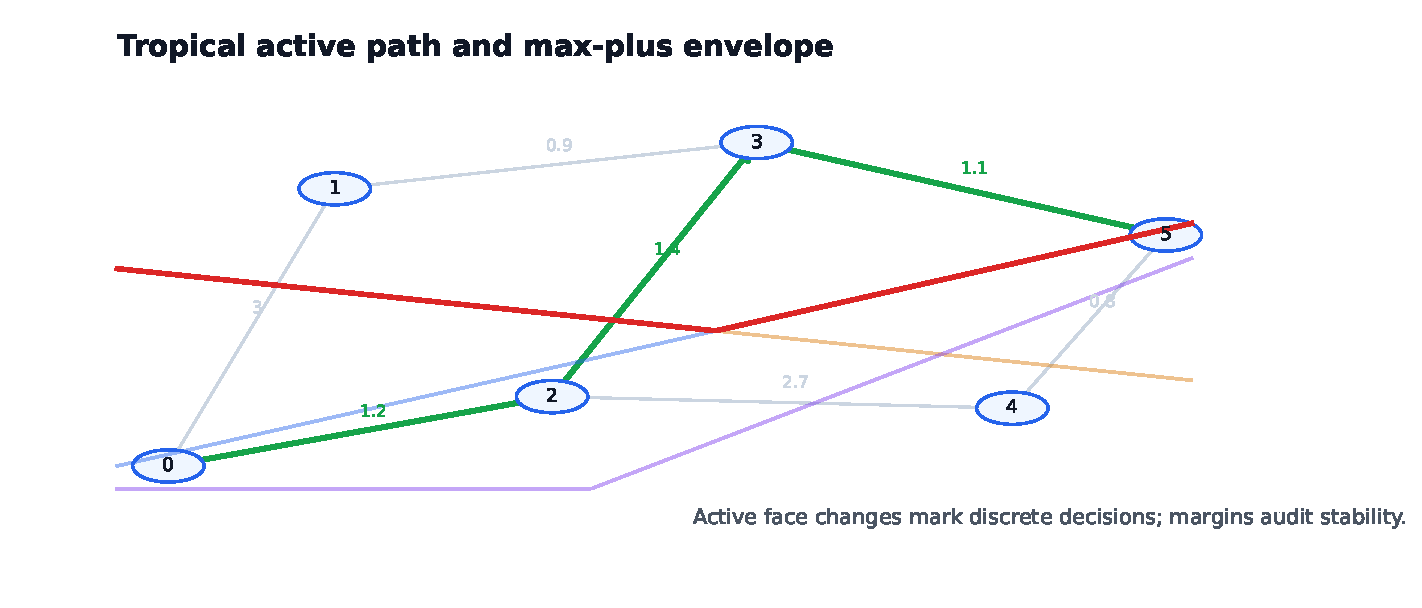
\includegraphics[width=\textwidth]{fig_tropical_active_faces.pdf}
  \caption{Tropical reasoning diagnostics.  Left: a shortest-path-style active predecessor path.  Right: a piecewise-linear tropical envelope whose active face and margin provide a direct explanation of a discrete decision.}
  \label{fig:tropical-active}
\end{figure}

\section{Toric geometry of neural-network charts}

The previous section treats tropical heads as max-plus computation.  A complementary view comes from toric geometry.  Fu's toric geometry of ReLU neural networks formalizes an observation that is directly useful for ToricGT: an unbiased rational ReLU network determines a polyhedral fan, a toric variety, and a Cartier divisor whose support function is the network output up to linear shift \cite{fu2025toricrelu}.  This section imports the part of that dictionary that is operational for a graph-token model.  The goal is not to make ToricGT an algebraic variety.  The goal is to expose the polyhedral and divisor-like structure already present in max-plus and ReLU subcomputations, and then use it as a diagnostic and a next-iteration training target.

\subsection{Minimal toric dictionary}

Let $N\simeq \Z^r$ be a cocharacter lattice and $M=\operatorname{Hom}(N,\Z)$ its character lattice, with pairing $\ip{m}{u}$ for $m\in M$ and $u\in N$ \cite{cox2011toric}.  A rational polyhedral cone is
\begin{equation}
  \sigma=\operatorname{Cone}(u_1,\ldots,u_s)
  =\left\{\sum_{j=1}^s\lambda_j u_j:\lambda_j\ge0,\ u_j\in N\right\}\subset N_\R.
\end{equation}
A fan $\Sigma$ is a finite collection of cones closed under faces and pairwise intersections.  A toric variety $X_\Sigma$ is glued from affine charts indexed by cones of $\Sigma$.  For this manuscript, the key combinatorial object is not the variety itself but the support function of a torus-invariant Cartier divisor:
\begin{equation}
  \varphi_D:|\Sigma|\to\R,\qquad
  \varphi_D(u)=\ip{m_\sigma}{u}\quad\text{for }u\in\sigma.
\end{equation}
The vectors $m_\sigma\in M$ are the Cartier data.  They are exactly the slopes of the piecewise-linear function on each maximal cone.  Across a shared wall $\tau=\sigma\cap\sigma'$, the difference $m_\sigma-m_{\sigma'}$ measures the bend of the support function.  In toric geometry this bend is encoded by the intersection number of $D$ with the torus-invariant curve $V(\tau)$; in a neural network it is the algebraic form of a kink.

\begin{definition}[Toric chart probe]
Let $H\in\R^{L\times d}$ be a graph-token hidden table.  A toric chart probe is a shared map
\begin{equation}
  \Pi(H_i)=\bigl(\ell_1(H_i),\ldots,\ell_R(H_i)\bigr),\qquad
  \ell_r(h)=\ip{a_r}{h}+b_r,
\end{equation}
where $a_r\in\Q^d$ after optional rational quantization.  Its tropical output is
\begin{equation}
  \psi(h)=\max_{r\le R}\ell_r(h).
\end{equation}
The associated Newton polytope is
\begin{equation}
  P_\Pi=\Conv(a_1,\ldots,a_R)\subset(\Q^d)^\ast.
\end{equation}
\end{definition}

The rationality condition is not a training restriction.  It is an audit restriction: a learned real-valued probe can be rounded to a rational lattice at evaluation time, just as finite Weyl-pair tasks approximate irrational rotations by rational phases.  This gives a reproducible, byte-stable object for visualization and comparison across checkpoints.

\begin{theorem}[Active faces are normal-fan cells]
\label{thm:active-normal-fan}
Let $\psi(h)=\max_r(\ip{a_r}{h}+b_r)$ and let
\begin{equation}
  A(h)=\argmax_r(\ip{a_r}{h}+b_r).
\end{equation}
For any active set $A$, define the lifted face
\begin{equation}
  F_A=\Conv\{(a_r,b_r):r\in A\}
  \subset(\Q^d)^\ast\times\Q.
\end{equation}
Then the set of hidden states with active set containing $A$ is a polyhedron cut out by linear inequalities
\begin{equation}
  \ip{a_r-a_s}{h}+b_r-b_s\ge0,
  \qquad r\in A,\ s\notin A.
\end{equation}
Equivalently, active-face diagnostics of a tropical head are cells in the normal fan of the lifted Newton polytope $\Conv\{(a_r,b_r)\}_{r=1}^R$.
\end{theorem}

\begin{proof}
The condition that $r$ is at least as good as $s$ is precisely
\begin{equation}
  \ip{a_r}{h}+b_r\ge \ip{a_s}{h}+b_s,
\end{equation}
which is a linear half-space condition in $h$.  Intersecting these half-spaces over all active candidates and inactive competitors gives the stated polyhedron.  A face of a polytope is exposed by a linear functional.  Here the functional is $(a,b)\mapsto \ip{a}{h}+b$, so candidates maximizing the tropical expression are exactly the vertices lying on the exposed face.  As $h$ varies, these exposed faces are organized by the normal fan.
\end{proof}

\begin{corollary}[Tropical margins are fan distances]
For a unique active candidate $r^\star$, the margin
\begin{equation}
  \Delta(h)=
  \min_{s\ne r^\star}\left[\ip{a_{r^\star}-a_s}{h}+b_{r^\star}-b_s\right]
\end{equation}
is the signed distance to the nearest wall of the active normal-fan cell, up to the norm of the corresponding wall normal.
\end{corollary}

\begin{proof}
The boundary between $r^\star$ and a competitor $s$ is the affine hyperplane
\begin{equation}
  \ip{a_{r^\star}-a_s}{h}+b_{r^\star}-b_s=0.
\end{equation}
The Euclidean distance to this hyperplane is the displayed affine value divided by $\norm{a_{r^\star}-a_s}_2$.  Taking the minimum over competitors gives the nearest wall.  Without the denominator, $\Delta(h)$ is the unnormalized signed fan distance.
\end{proof}

\begin{figure}[t]
  \centering
  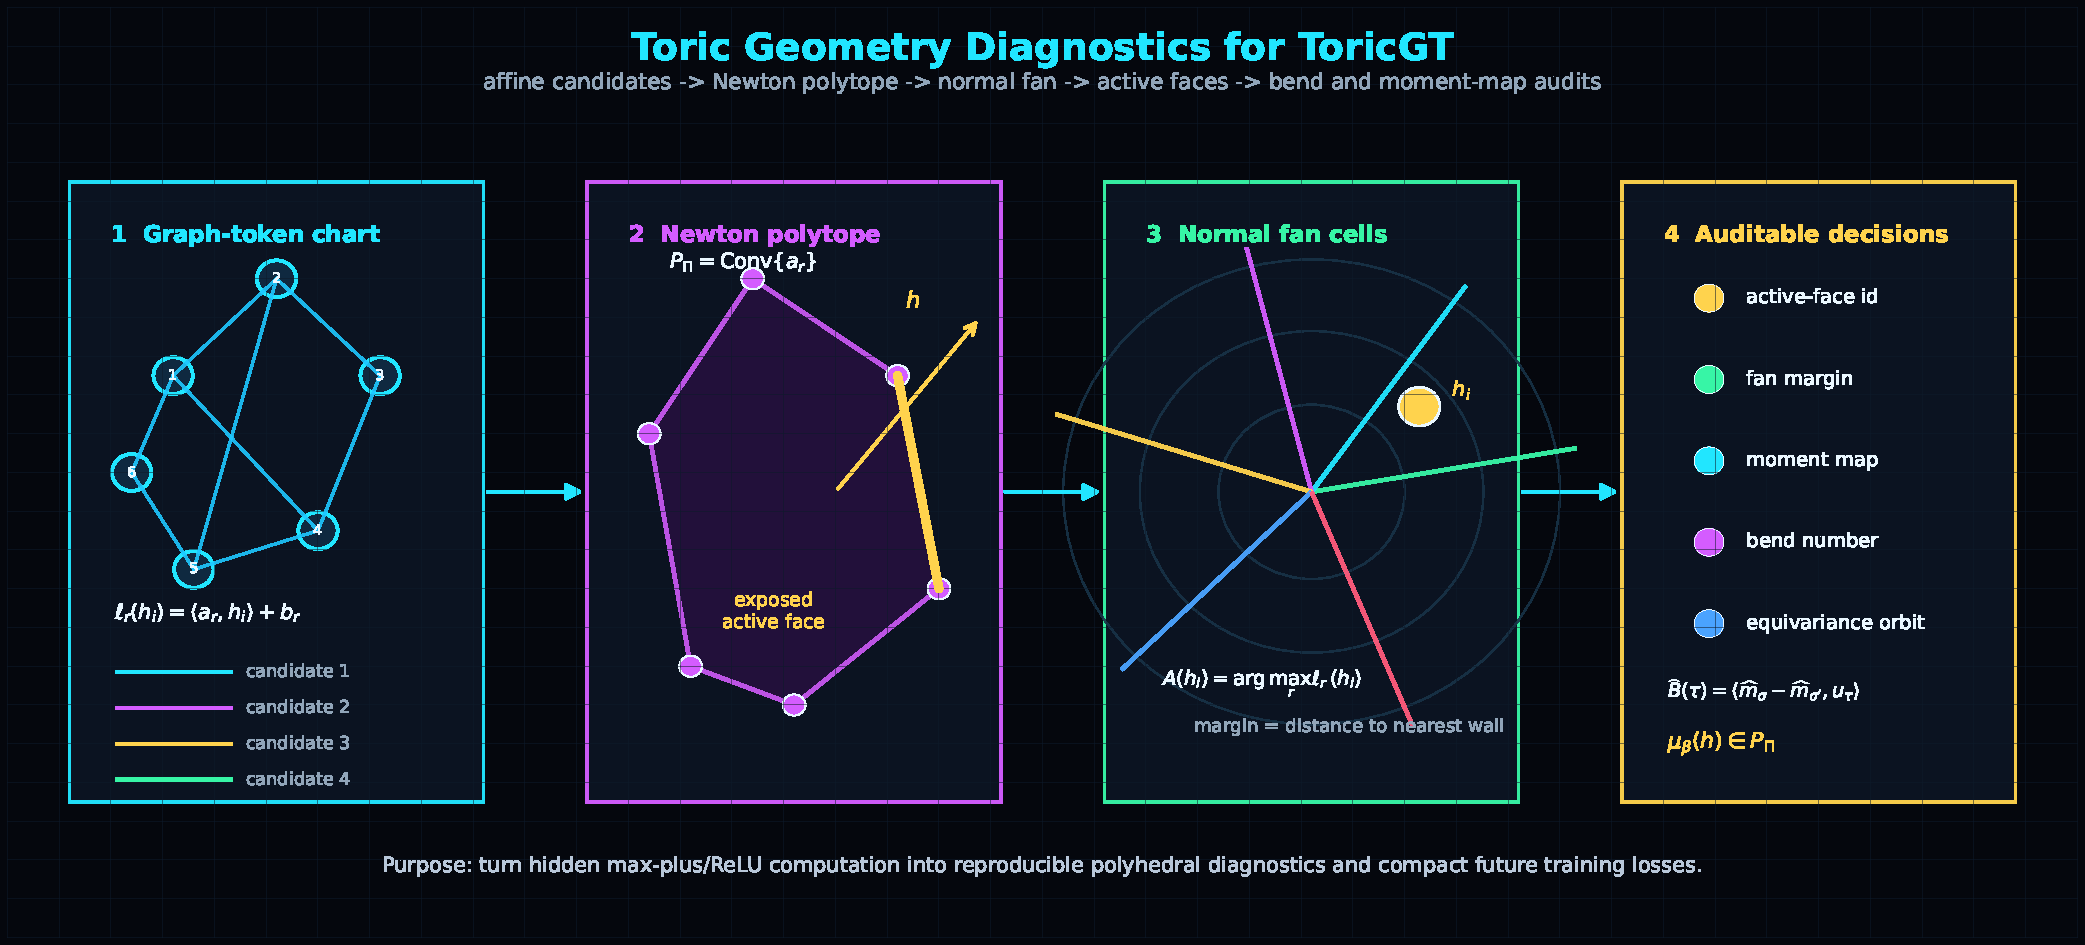
\includegraphics[width=\textwidth]{fig_toric_geometry_relu_toricgt.pdf}
  \caption{Toric-geometric interpretation of ToricGT tropical subcomputations.  A graph-token hidden state is scored by affine candidates.  Their exponent vectors form a Newton polytope; its normal fan partitions hidden space into active regions.  Active faces and bend numbers become diagnostics for reasoning decisions and future toric auxiliary losses.}
  \label{fig:toric-geometry-toricgt}
\end{figure}

\subsection{ReLU fans, Cartier data, and ToricGT diagnostics}

A feed-forward ReLU network is continuous piecewise linear.  Fu defines its ReLU fan $\Sigma_{f_\theta}$ as the canonical polyhedral complex on which all hidden-layer piecewise-linear functions and the output are linear.  The corresponding ReLU toric variety is $X_{\Sigma_{f_\theta}}$, and the output function is the support function of a ReLU Cartier divisor $D_f$ on that fan \cite{fu2025toricrelu}.  Zhang, Naitzat, and Lim earlier showed that ReLU networks can be represented as tropical rational maps and that their decision boundaries are controlled by tropical hypersurfaces \cite{zhang2018tropical}.  Later work uses activation polytopes and classification fans to study real tropical decision regions \cite{brandenburg2024real}, and lattice-polytope arguments give depth lower bounds for integral ReLU networks \cite{haase2023lattice}.  The toric view refines this by giving a divisor and intersection-number language for the same bends.

ToricGT contains two sources of piecewise-linear structure.  First, tropical attention heads are explicitly max-plus.  Second, ordinary feed-forward and Soft-MoE expert sublayers often use ReLU or GELU-like gates; ReLU subpaths admit exact fan descriptions, while smooth gates admit local linearization or temperature-controlled max approximations.  For a fixed checkpoint and a bounded evaluation corpus, one can attach an \emph{empirical ReLU fan} to any probe subnetwork by clustering hidden states according to activation signs and tropical active faces.

\begin{definition}[Empirical toric shadow]
Fix a bounded batch family $\mathcal B$ and a ToricGT checkpoint.  Let $\mathcal A(h)$ collect the binary ReLU activation pattern, tropical active-face pattern, and Soft-MoE dominant-slot pattern of a chosen subnetwork at hidden state $h$.  The empirical toric shadow is the finite cell decomposition
\begin{equation}
  \widehat\Sigma_{\mathcal B}=\{\,\{h\in\mathcal B:\mathcal A(h)=a\}:a\in\operatorname{im}\mathcal A\,\},
\end{equation}
equipped with fitted local slopes $\widehat m_\sigma$ for each occupied cell $\sigma$.
\end{definition}

Local slopes can be estimated by least squares over hidden-state/output pairs inside a cell:
\begin{equation}
  \widehat m_\sigma
  =\argmin_m\sum_{h_i\in\sigma}\abs{\psi(h_i)-\ip{m}{h_i}}^2.
\end{equation}
The fitted slopes are not used to prove exact representability of the learned model.  They are used to inspect whether the checkpoint has learned stable polyhedral computation: low within-cell residual, large fan margins, repeated bend patterns across equivalent graph situations, and coherent Newton-polytopal active faces.

\begin{proposition}[Equivariance of toric shadows]
Assume the probe, attention masks, tropical heads, and Soft-MoE routers are shared over token rows and have no absolute token-index input.  If $P_\pi$ is a graph-token relabeling, then the empirical toric shadow of $\pi G$ is the row-permuted shadow of $G$.  In particular, the multiset of Newton polytopes, active-face dimensions, tropical margins, and fitted bend magnitudes is invariant under graph relabeling.
\end{proposition}

\begin{proof}
By tokenization and block equivariance, hidden states transform by row permutation.  Shared probes and routers therefore produce the same activation, slot, and active-face labels on permuted rows.  The Newton polytope of a shared probe depends only on its candidate slopes, not on row order.  Least-squares slope fitting within a cell is unchanged after relabeling because the objective is a sum over the same points in permuted order.  Hence all listed diagnostics are invariant as multisets, with only token labels permuted.
\end{proof}

\begin{definition}[Bend audit]
Let $\sigma,\sigma'$ be adjacent occupied cells in an empirical toric shadow, with shared wall normal $u_{\tau}$ after rational approximation.  The empirical bend across the wall $\tau=\sigma\cap\sigma'$ is
\begin{equation}
  \widehat B(\tau)=\ip{\widehat m_\sigma-\widehat m_{\sigma'}}{u_\tau}.
\end{equation}
\end{definition}

In the exact toric setting, this quantity is the intersection number of the corresponding Cartier divisor with the torus-invariant curve $V(\tau)$.  For ToricGT it becomes a diagnostic for whether reasoning decisions change consistently across equivalent graph perturbations.  For example, in a shortest-path task, crossing a wall that changes the active predecessor should produce a bend aligned with the edge-weight difference.  In a Hebrew root-template alignment task, crossing a wall that changes a radical-slot assignment should produce a bend localized to the relevant template slot, not a global drift across unrelated graph tokens.

\subsection{Moment features and compact toric regularization}

Toric geometry also suggests a compact way to summarize a tropical decision.  Given affine candidates $\ell_r(h)=\ip{a_r}{h}+b_r$ and inverse temperature $\beta>0$, define the soft active-face moment
\begin{equation}
  \mu_\beta(h)=
  \frac{\sum_{r=1}^R \exp(\beta\ell_r(h))a_r}
       {\sum_{r=1}^R \exp(\beta\ell_r(h))}
  \in P_\Pi.
\end{equation}
This is the moment-map analogue of a softmax over candidate exponents.  As $\beta\to\infty$, $\mu_\beta(h)$ converges to a convex combination of the active vertices of the Newton polytope.

\begin{lemma}[Moment map limit]
If $A(h)$ is the active set of $\psi(h)=\max_r\ell_r(h)$, then every accumulation point of $\mu_\beta(h)$ as $\beta\to\infty$ lies in $\Conv\{a_r:r\in A(h)\}$.  If the active maximizer is unique, $\mu_\beta(h)\to a_{r^\star}$.
\end{lemma}

\begin{proof}
Write $M=\max_r\ell_r(h)$.  Terms with $r\notin A(h)$ are multiplied by $\exp(\beta(\ell_r(h)-M))$, which converges to $0$.  Terms with $r\in A(h)$ all have exponent $0$ after factoring out $\exp(\beta M)$.  Therefore the limit is a normalized convex combination of active $a_r$'s.  If $A(h)=\{r^\star\}$, only one term remains.
\end{proof}

This gives a low-cost diagnostic for compact models.  Rather than storing large explanation traces, a Parameter-Golf-facing model can emit quantized moments $\mu_\beta(h)$, active-face ids, and top-two margins.  These are enough to audit whether the small model uses stable polyhedral decisions without increasing the artifact by a large expert bank.

\subsection{Toric auxiliary losses for training}

The toric view suggests auxiliary losses that do not require changing the deployable architecture.  They are attached as training-only low-rank probes and excluded from the compressed artifact unless a later ablation justifies their byte cost.  Let $\mathcal R$ be a set of integer relations among exponent vectors,
\begin{equation}
  \sum_r \alpha_r a_r=\sum_r \beta_r a_r,
  \qquad \alpha_r,\beta_r\in\N.
\end{equation}
In log-coordinate form, the associated binomial consistency loss is
\begin{equation}
  \mathcal L_{\mathrm{binom}}
  =
  \sum_{(\alpha,\beta)\in\mathcal R}
  \left\|
    \sum_r\alpha_r \ell_r(h)-\sum_r\beta_r \ell_r(h)
  \right\|_2^2.
\end{equation}
For active-face stability, a fan-margin loss can be used:
\begin{equation}
  \mathcal L_{\mathrm{fan}}
  =
  \Eop_h\max\left(0,\gamma-
  \min_{s\notin A(h),\,r\in A(h)}
  \bigl[\ell_r(h)-\ell_s(h)\bigr]\right).
\end{equation}
For repeated graph situations expected to share the same bend, use
\begin{equation}
  \mathcal L_{\mathrm{bend}}
  =
  \sum_{(\tau,\tau')\in\mathcal P}
  \abs{\widehat B(\tau)-\widehat B(\tau')}^2,
\end{equation}
where $\mathcal P$ pairs walls that are equivalent under graph relabeling, algebraic normal form, or morphology-template symmetry.  These losses are pragmatic: they regularize the geometry of reasoning decisions rather than merely increasing parameter count.

The implemented compact objective also adds affine-Coxeter, braid, and phase-leaf terms:
\begin{equation}
\begin{split}
  \mathcal L_{\mathrm{toric}}
  ={}&\mathcal L_{\mathrm{base}}
  +\lambda_{\mathrm{fan}}\mathcal L_{\mathrm{fan}}
  +\lambda_{\mathrm{bend}}\mathcal L_{\mathrm{bend}}
  +\lambda_{\mathrm{binom}}\mathcal L_{\mathrm{binom}}
  +\lambda_{\mathrm{moment}}\norm{\widehat\mu-\mu^\star}_2^2\\
  &+\lambda_{\mathrm{cox}}\mathcal L_{\mathrm{cox}}
  +\lambda_{\mathrm{br}}\mathcal L_{\mathrm{br}}
  +\lambda_{\mathrm{leaf}}\mathcal L_{\mathrm{leaf}}.
\end{split}
\end{equation}
Here $\mathcal L_{\mathrm{cox}}$ reflects predicted and teacher moments across simple affine walls and compares the reflected points, $\mathcal L_{\mathrm{br}}$ compares the two length-three braid paths $s_1s_2s_1$ and $s_2s_1s_2$, and $\mathcal L_{\mathrm{leaf}}$ compares successive projected phase increments with the irrational rotation increments determined by $(\theta,\beta)$.  The probe is low-rank and fake-quantized during training, so it tests whether the main hidden state contains a compact toric chart rather than adding a large explanation module.  The evaluation suite separately builds empirical toric shadows from hidden states alone: occupied fan cells, active-face margins, bend magnitudes, fitted-slope residuals, and branch-wise phase-leaf residuals.  Thus old checkpoints can be audited even when they were trained before the probe existed.


\section{Toric BGG structure as trainable supervision}\label{sec:toric-bgg}

The toric layer above gives polyhedral charts for hidden computation.  This section adds the representation-theoretic layer that was missing from the earlier specification: hypertoric category $\mathcal O$, oriented-matroid category $\mathcal O$, and multigraded BGG/Tate resolutions provide finite algebraic templates that can be used as training signals.  The proposal is deliberately modest.  ToricGT is not claimed to learn an abelian or derived category in any literal sense.  Instead, each minibatch can carry small certificate objects - sign-vector posets, standard filtrations, chain complexes, multigraded Betti vectors, Gale-dual labels, and toric differential modules - whose algebraic identities are exact, cheap to verify, and aligned with the model's existing graph-token, tropical, GraphCG, and trajectory-memory components.

The gain is conceptual and practical.  BGG theory supplies a disciplined language for reasoning by standard objects, resolutions, and exact functors.  In model terms, a reasoning trajectory should not be a shapeless string of latent states.  It should be close to a chain complex; its local moves should resemble differentials; its reusable subroutines should behave like standard modules; and analogical transfer should look like an approximate exact functor between two finite proxy categories.  These requirements are stronger than ordinary next-token likelihood, but they can be applied with low-rank probes and discarded at export.  This is exactly the regime in which a BPB-constrained model needs auxiliary structure: improve the representation during training without paying a large byte cost at evaluation.

\subsection{Three BGG inputs and what they contribute}

There are three mathematical sources.  They have different roles and should not be conflated.

First, classical Bernstein-Gelfand-Gelfand category $\mathcal O$ for a complex semisimple Lie algebra is the prototype.  It is a highest-weight category with Verma modules, simple modules, projective covers, BGG reciprocity, and BGG resolutions of finite-dimensional simple modules by Verma modules \cite{bgg1976category}.  For ToricGT, the important lesson is not the Lie algebra itself, but the use of a partially ordered set of weights and standard objects to organize reasoning.

Second, hypertoric category $\mathcal O$ is the genuinely toric BGG analogue.  Braden, Licata, Proudfoot, and Webster define category $\mathcal O$ for hypertoric enveloping algebras, identify it with sheaf-theoretic categories on hypertoric varieties, and prove highest-weight and Koszul properties for regular blocks; their general theory of category $\mathcal O$ for quantized conical symplectic resolutions extends the same pattern to a larger symplectic-geometric class \cite{braden2012hypertoric,braden2016qcsr}.  Hypertoric data are controlled by hyperplane arrangements and their Gale duals, hence by finite combinatorics that can be used during training.

Third, multigraded BGG and toric Tate resolutions move from representation theory to toric commutative algebra.  Brown and Erman develop Tate resolutions on projective toric varieties, and the multigraded BGG correspondence has a computational implementation in Macaulay2 through differential exterior modules and their resolutions \cite{brownerman2022tate,banks2025multigradedbgg}.  This source is especially useful for code: one can generate small graded modules, compute free resolutions or strongly linear strands offline, and convert the result into graph-token training records.

These sources share a common finite skeleton: a poset or fan, a family of standard generators, differentials along covers or incidence relations, and homological constraints such as $d^2=0$, linearity, exactness, and Koszulity.  The ToricGT objective below uses only that skeleton.

\begin{definition}[Highest-weight training skeleton]\label{def:hw-skeleton}
A highest-weight training skeleton is a finite tuple
\begin{equation}
  \mathfrak S=(\Lambda,\leq,\mathcal G,\mathcal D,\deg,\omega),
\end{equation}
where $(\Lambda,\leq)$ is a finite poset, $\mathcal G$ is a finite set of generators called standard tokens, $\mathcal D=\{D_k:C_k\to C_{k-1}\}$ is a graded chain complex whose basis elements are labeled by elements of $\Lambda$, $\deg$ is an internal grading, and $\omega$ is metadata recording the source of the skeleton: classical BGG, hypertoric arrangement, oriented matroid, toric Tate resolution, Euler-Koszul complex, or a synthetic proxy.  The skeleton is \emph{valid} if $D_{k-1}D_k=0$ for all $k$ and every basis label has a well-defined order relation to every standard token it can attend to.
\end{definition}

The skeleton is small.  A typical minibatch certificate has between 8 and 256 basis elements.  It is not a symbolic algebra system embedded in the model.  It is a supervision object analogous to a parse tree or proof graph, except that its invariants come from module theory.

\begin{definition}[Hypertoric arrangement certificate]\label{def:hypertoric-certificate}
Let $A\in\Z^{d\times n}$ have rank $d$, and let $T=(\C^*)^d$ act on $V=\C^n$ with weights given by the columns of $A$.  Write $\mu:T^*V\to\mathfrak t^*$ for the moment map.  For a stability parameter $\eta$, the hypertoric variety is
\begin{equation}
  \mathfrak M_\eta(A)=\mu^{-1}(0) /
\!/_\eta T.
\end{equation}
A hypertoric arrangement certificate is the finite combinatorial package
\begin{equation}
  \mathcal C_A=(\mathcal L_A,\mathcal B_A,\mathcal F_A,\mathcal P_A,\mathcal G_A),
\end{equation}
where $\mathcal L_A$ is the oriented-matroid sign-vector set, $\mathcal B_A$ is the set of bounded feasible sign vectors for the chosen generic program, $\mathcal F_A$ is the face poset induced by covector specialization, $\mathcal P_A$ is the standard-object poset used for category-$\mathcal O$ supervision, and $\mathcal G_A$ is a Gale-dual certificate for a matrix $B$ whose columns present the kernel of $A$.
\end{definition}

In the realizable case this certificate is a finite shadow of hypertoric category $\mathcal O$.  In the nonrealizable case it is an oriented-matroid proxy; Kowalenko and Mautner's construction shows that category-$\mathcal O$-like algebras exist for sufficiently generic oriented matroid programs and recover the Braden-Licata-Proudfoot-Webster algebra in the linear arrangement case \cite{kowalenko2022oriented}.  For training, this distinction matters because nonrealizable oriented matroids provide harder combinatorial out-of-distribution tests without requiring real coordinates.

\subsection{Finite proxy algebras}

The exact BLPW algebra is valuable mathematically, but it is more machinery than is needed inside a minibatch.  The train-time proxy should be an algebra whose objects can be built in Python from sign vectors and whose homological checks are exact over a small field.  The following incidence model is the default.

\begin{definition}[Incidence proxy algebra]\label{def:incidence-proxy}
Let $P$ be a finite poset and let $k$ be a field.  The incidence algebra $I(P;k)$ has basis $e_{xy}$ for $x\leq y$, with multiplication
\begin{equation}
  e_{xy}e_{uv}=\begin{cases}
    e_{xv}, & y=u,\\
    0, & y\ne u.
  \end{cases}
\end{equation}
The idempotent $e_x=e_{xx}$ labels a simple module $L_x$.  The right projective module $P_x=e_xI(P;k)$ has basis $\{e_{xy}:x\le y\}$.
\end{definition}

\begin{proposition}[Projective factors in the incidence proxy]\label{prop:incidence-factors}
For the right incidence algebra convention above, the indecomposable projective $P_x=e_xI(P;k)$ has one composition factor $L_y$ for each $y\in P$ satisfying $x\le y$, and no other composition factors.
\end{proposition}

\begin{proof}
The module $P_x$ is spanned by intervals $e_{xy}$ with $x\le y$.  Let $P_x^{\ge z}$ be the span of basis elements $e_{xy}$ with $y\ge z$ for a chosen linear extension of $P$.  Ordering the endpoints $y$ by any linear extension compatible with $\leq$ gives a filtration whose successive quotients are one-dimensional.  Right multiplication by an idempotent $e_u$ acts on $e_{xy}$ by $e_{xy}e_u=e_{xy}$ if $u=y$ and by $0$ otherwise.  Therefore the quotient generated by the class of $e_{xy}$ is the simple module $L_y$.  Every endpoint $y\ge x$ occurs once, and no endpoint outside the principal filter of $x$ occurs in the basis.
\end{proof}

This proxy is deliberately transparent.  The model sees the same partial order that governs the standard modules, and the training code can compute projective-factor labels without symbolic algebra.  The proxy does not replace hypertoric category $\mathcal O$; it gives a safe finite target whose errors can be inspected and whose ablations are cheap.

\begin{definition}[Standard-attention mask]\label{def:standard-mask}
Let $H=(h_\lambda)_{\lambda\in\Lambda}$ be hidden states indexed by a finite highest-weight skeleton.  The standard-attention mask is
\begin{equation}
  M_{\lambda\mu}^{\mathrm{std}}=\begin{cases}
    0,& \mu\leq \lambda,\\
    -\infty,& \text{otherwise.}
  \end{cases}
\end{equation}
A soft version replaces $-\infty$ by a large negative constant and reports the leakage mass
\begin{equation}
  \mathrm{Leak}_{\mathrm{std}}(H)=\frac{1}{|\Lambda|}\sum_{\lambda}\sum_{\mu\not\leq\lambda}\mathrm{Attn}_{\lambda\mu}.
\end{equation}
\end{definition}

\begin{lemma}[Standard masks are equivariant under poset automorphisms]\label{lem:std-mask-equiv}
If $\pi$ is an automorphism of $(\Lambda,\leq)$ and $P_\pi$ is the corresponding permutation matrix, then
\begin{equation}
  M^{\mathrm{std}}(\pi\Lambda)=P_\pi M^{\mathrm{std}}(\Lambda)P_\pi^T.
\end{equation}
Consequently a ToricGT block with shared projections and standard masks remains equivariant with respect to automorphisms of the skeleton.
\end{lemma}

\begin{proof}
The entry $M_{\lambda\mu}^{\mathrm{std}}$ is unmasked exactly when $\mu\leq\lambda$.  Since $\pi$ is a poset automorphism, $\mu\leq\lambda$ if and only if $\pi\mu\leq\pi\lambda$.  Thus the unmasked pairs are exactly carried to their permuted unmasked pairs.  This is precisely conjugation by $P_\pi$.  The attention equivariance proof from the graph-token section then applies verbatim.
\end{proof}

\subsection{The multigraded BGG differential}

The most implementation-friendly BGG object is the differential module associated with a multigraded polynomial ring.  It gives exact $d^2=0$ labels and linear-strand supervision for hidden trajectories.

\begin{definition}[Multigraded BGG differential]\label{def:multigraded-bgg-diff}
Let $S=k[x_1,\ldots,x_n]$ be graded by an abelian group $G$, and let $E=\bigwedge_k(e_1,\ldots,e_n)$ be the exterior algebra with dual multidegrees $\deg e_i=-\deg x_i$.  For a $G$-graded $S$-module $M$, define the BGG differential on $M\otimes_k E$ by
\begin{equation}
  d(m\otimes \xi)=\sum_{i=1}^n x_i m\otimes e_i\wedge \xi.
\end{equation}
When $M$ already carries a differential, this is combined with the internal differential with the usual Koszul sign convention.
\end{definition}

\begin{lemma}[BGG differential squares to zero]\label{lem:bgg-d2}
For an ordinary graded $S$-module $M$ with no internal differential, the map $d$ in \cref{def:multigraded-bgg-diff} satisfies $d^2=0$.
\end{lemma}

\begin{proof}
For $m\otimes\xi\in M\otimes E$,
\begin{equation}
  d^2(m\otimes\xi)=\sum_{i,j}x_jx_i m\otimes e_j\wedge e_i\wedge \xi.
\end{equation}
The terms with $i=j$ vanish because $e_i\wedge e_i=0$.  For $i\ne j$, the pair $(i,j)$ cancels the pair $(j,i)$: the polynomial variables commute, $x_jx_i=x_ix_j$, while the exterior generators anticommute, $e_j\wedge e_i=-e_i\wedge e_j$.  Hence the full sum is zero.
\end{proof}

\begin{example}[A two-variable computation]\label{ex:bgg-two-var}
Let $S=k[x,y]$, $E=\bigwedge(e_x,e_y)$, and $M=k=S/(x,y)$.  The BGG complex is the Koszul complex
\begin{equation}
  0\longrightarrow S(-2)\xrightarrow{\begin{bmatrix}-y\\x\end{bmatrix}}S(-1)^2\xrightarrow{\begin{bmatrix}x&y\end{bmatrix}}S\longrightarrow k\longrightarrow0.
\end{equation}
The composition is $[x\ y][-y\ x]^T=-xy+yx=0$.  For a graph-token model, this is a minimal sanity record: the hidden differential must send the degree-two basis token to two degree-one basis tokens with opposite signed monomial labels, and the next differential must annihilate the result.  A model that fails this example should not receive more elaborate toric BGG supervision.
\end{example}

\begin{definition}[Resolution-consistency loss]\label{def:resolution-loss}
Let a minibatch certificate provide matrices $D_k^\star$ over a field $k$ or over $\R$ after embedding signs and monomial labels.  Let a ToricGT probe predict matrices $\widehat D_k(H)$ from hidden states.  The resolution-consistency loss is
\begin{equation}
  \mathcal L_{\partial^2}=\sum_k\norm{\widehat D_{k-1}\widehat D_k}_F^2,
\end{equation}
with optional supervised alignment
\begin{equation}
  \mathcal L_D=\sum_k\norm{\widehat D_k-D_k^\star}_F^2.
\end{equation}
When only the homology type is known, $\mathcal L_D$ is omitted and exactness is audited by ranks over a small finite field.
\end{definition}

\begin{proposition}[Stable chain-map supervision]\label{prop:stable-chain-map}
Let $C_\bullet$ and $C'_\bullet$ be finite chain complexes with differentials $d,d'$ and operator norms at most $R$.  Suppose maps $F_k:C_k\to C'_k$ satisfy
\begin{equation}
  \norm{d'F_k-F_{k-1}d}\leq\epsilon
\end{equation}
for all $k$.  If $z\in C_k$ is a cycle with $\norm{z}\leq1$, then $F_kz$ is within $\epsilon$ of a cycle in the sense that $\norm{d'F_kz}\leq\epsilon$.  If $z=d w$ with $\norm{w}\leq1$, then $F_kz$ is within $\epsilon$ of the boundary $d'F_{k+1}w$.
\end{proposition}

\begin{proof}
If $dz=0$, then
\begin{equation}
  \norm{d'F_kz}=\norm{(d'F_k-F_{k-1}d)z}\leq\epsilon\norm{z}\leq\epsilon.
\end{equation}
If $z=dw$, then
\begin{equation}
  F_kz=F_kdw=d'F_{k+1}w-(d'F_{k+1}-F_kd)w,
\end{equation}
so $F_kz$ differs from the boundary $d'F_{k+1}w$ by a vector of norm at most $\epsilon$.
\end{proof}

This proposition is the mathematical justification for treating analogical reasoning as an approximate exact functor.  The model need not reconstruct a whole category.  It must learn maps between finite complexes that send cycles nearly to cycles and boundaries nearly to boundaries.

\subsection{Gale duality and Koszul dual curricula}

Hypertoric category $\mathcal O$ is especially attractive because the Koszul dual is controlled by Gale duality.  This gives a natural paired curriculum: solve a task for an arrangement, solve the dual task for the Gale-dual arrangement, and penalize contradictions between the two hidden signatures.

\begin{definition}[Gale-dual training pair]\label{def:gale-pair}
Let $A\in\Z^{d\times n}$ have rank $d$.  A Gale dual is an integer matrix $B\in\Z^{(n-d)\times n}$ whose rows span the lattice of integer relations among the columns of $A$, so that
\begin{equation}
  0\longrightarrow \Z^{n-d}\xrightarrow{B^T}\Z^n\xrightarrow{A}\Z^d\longrightarrow 0
\end{equation}
is exact after passing to the appropriate saturated lattice.  A Gale-dual training pair consists of certificates $\mathcal C_A$ and $\mathcal C_B$ together with a label map that identifies bases of the matroid of $A$ with complements of bases of the matroid of $B$.
\end{definition}

\begin{lemma}[Basis complementarity]\label{lem:basis-complementarity}
Assume $A$ represents a rank-$d$ matroid on $[n]$ and $B$ represents its Gale dual matroid of rank $n-d$.  A subset $I\subset[n]$ is a basis for $A$ if and only if $[n]\setminus I$ is a basis for $B$.
\end{lemma}

\begin{proof}
The columns indexed by $I$ form a basis for the quotient map $\Z^n\to\Z^d$ precisely when the coordinate subspace on $[n]\setminus I$ intersects the kernel trivially and has complementary rank.  The kernel is represented by the rows of $B$, so the complementary coordinates $[n]\setminus I$ carry full rank for the dual representation.  This is the standard basis-complement characterization of matroid duality.
\end{proof}

\begin{definition}[Gale-dual consistency loss]\label{def:gale-loss}
Let $s_A(H)$ and $s_B(H')$ be learned signatures for paired examples from $A$ and its Gale dual $B$.  Each signature includes a Betti vector, active-face histogram, standard-filtration mass, and trajectory-memory key.  The Gale-dual consistency loss is
\begin{equation}
  \mathcal L_{\mathrm{Gale}}=\norm{G_\theta s_A(H)-s_B(H')}_2^2+\norm{G_\theta^{-1}s_B(H')-s_A(H)}_2^2,
\end{equation}
where $G_\theta$ is a small learned orthogonal or low-rank map initialized from the combinatorial complement map.
\end{definition}

The loss is low risk when used late.  If it helps, the model has learned a reusable duality between two finite reasoning problems.  If it does not, the loss can be disabled without changing the base architecture.

\subsection{Euler-Koszul probes and toric module theory}

Toric $D$-module theory supplies a second family of certificates.  These are not needed for every ToricGT run, but they are useful for tasks involving toric ideals, semigroup rings, and hypergeometric recurrences.

\begin{definition}[Toric module and Euler-Koszul certificate]\label{def:euler-koszul-cert}
Let $A=[a_1\cdots a_n]\in\Z^{d\times n}$ and let $S_A=k[\N A]$ be the affine semigroup ring.  A toric module is a $\Z^d$-graded module built from $S_A$ and its face quotients by extensions.  For a parameter $\beta\in k^d$, the Euler operators are
\begin{equation}
  E_i-\beta_i=\sum_{j=1}^n a_{ij}x_j\partial_j-\beta_i.
\end{equation}
An Euler-Koszul certificate is the Koszul complex $K_\bullet(E-\beta;M)$ of these commuting operators acting on a toric module $M$.
\end{definition}

Matusevich, Miller, and Walther developed Euler-Koszul homology for toric modules in the study of hypergeometric families, and later work relates these complexes to $D$-module direct images and toric geometry \cite{matusevich2005homological,schulze2009hypergeometric}.  For ToricGT, the practical use is simple: the certificate supplies commuting operators and a Koszul complex.  The model can be trained to predict when the complex is exact, when resonance causes homology, and how toric relations change the solution space.

\begin{proposition}[Commuting Euler operators give a Koszul complex]\label{prop:euler-koszul}
If the operators $T_1,\ldots,T_d$ commute on a module $M$, then the Koszul differential on
\begin{equation}
  K_q(T;M)=M\otimes \bigwedge^q k^d
\end{equation}
satisfies $d^2=0$.
\end{proposition}

\begin{proof}
The differential is
\begin{equation}
  d(m\otimes e_{i_1}\wedge\cdots\wedge e_{i_q})=\sum_{s=1}^q(-1)^{s-1}T_{i_s}m\otimes e_{i_1}\wedge\cdots\widehat{e_{i_s}}\cdots\wedge e_{i_q}.
\end{equation}
Applying $d$ twice gives a signed sum over ordered pairs $(i_r,i_s)$.  The two orders have opposite exterior signs, and the module operators commute, $T_iT_j=T_jT_i$.  Hence every pair cancels.
\end{proof}

\subsection{Embedding-space realization: BGG signatures for GraphCG and memory}

ToricGT already uses GraphCG-style concept charts and a trajectory-memory head.  Toric BGG supervision should enter through those modules rather than bypassing them.

Let $B=[d_1,\ldots,d_r]\in\R^{d\times r}$ be the GraphCG chart and $\xi=B^Th$ the concept coordinate.  For a skeleton $\mathfrak S$ with labels $\lambda\in\Lambda$, attach to each label a learned standard vector $u_\lambda\in\R^r$ and define
\begin{equation}
  p(\lambda\mid h)=\softmax_\lambda\left(\frac{\ip{u_\lambda}{B^Th}+b_\lambda}{\tau}\right).
\end{equation}
The standard-purity score of a hidden trajectory $H=(h_t)$ is
\begin{equation}
  \mathrm{Pur}_{\mathcal O}(H)=1-\frac{1}{T}\sum_{t=1}^T\sum_{\mu\not\leq \lambda_t}p(\mu\mid h_t),
\end{equation}
where $\lambda_t$ is the certificate label at step $t$.  High purity means that GraphCG axes have aligned with the order ideals of the standard-module skeleton.

\begin{definition}[Toric BGG trajectory signature]\label{def:bgg-signature}
For a completed graph-of-thought trajectory $\tau$, define
\begin{equation}
  \Sigma_{\mathrm{TBGG}}(\tau)=\bigl(\mathbf b(\tau),\,\mathbf e(\tau),\,\mathbf f(\tau),\,\mathbf g(\tau),\,\mathbf m(\tau),\,\mathbf p(\tau),\,q(\tau)\bigr),
\end{equation}
where $\mathbf b$ is a multigraded Betti or homology-rank vector, $\mathbf e$ is an Ext-degree histogram, $\mathbf f$ is a fan-cell path, $\mathbf g$ is the Gale-dual label vector, $\mathbf m$ is the moment-map summary, $\mathbf p$ is the noncommutative phase summary, and $q(\tau)$ is a scalar quality score such as verifier reward or negative local BPB.  The memory key used by retrieval is the normalized concatenation of this signature with the existing endpoint, curvature, and topology statistics.
\end{definition}

\begin{proposition}[Analogy invariance of exact BGG signatures]\label{prop:analogy-signature}
Let $F:C_\bullet\to C'_\bullet$ be an isomorphism of finite labeled chain complexes preserving homological degree, internal degree, poset order, and Gale-dual labels.  Then the Betti vector, Ext-degree histogram, standard-filtration multiplicities, and exact fan-cell adjacency pattern of $C_\bullet$ and $C'_\bullet$ agree after relabeling.
\end{proposition}

\begin{proof}
An isomorphism of chain complexes preserves the ranks of cycles, boundaries, and homology in each degree.  Since internal degree is preserved, the multigraded Betti vector is preserved degree by degree.  The Ext-degree histogram is computed from a projective or free resolution, and isomorphism of labeled complexes carries the resolution data to the corresponding relabeled data.  Poset-order preservation gives the same standard-filtration multiplicities.  Fan-cell adjacency is a relation on labels and faces; a label-preserving isomorphism transports adjacent labels to adjacent labels.  Thus all stated components agree after relabeling.
\end{proof}

This proposition explains why BGG signatures are useful memory keys.  A helper trajectory that is isomorphic as a finite complex is not just semantically similar; it carries the same resolution structure.  That is a stronger retrieval criterion than cosine similarity of final hidden states.

\subsection{Behavior protocols from toric-tropical corridors and algebraic certificates}
\label{subsec:behavior-corridors-bgg}

The same finite certificate machinery can be used for behavior modification in a precise and auditable sense.  The goal is to constrain the model's hidden graph-of-thought trajectory to regions associated with wanted behavior--helpfulness, calibrated accuracy, groundedness, appropriate tone, suitable amount of detail, mathematical rigor, and safe refusal when needed--while avoiding regions associated with unwanted behavior such as unsafe compliance, sycophancy, hallucination, brittle persona drift, or ungrounded overconfidence.  Anthropic's Assistant Axis identifies a single contrast direction in activation space and treats activation capping as a way to keep the model near its default Assistant persona \cite{lu2026assistantaxis}.  ToricGT uses that axis as a baseline special case.  The general object is a chamberwise toric-tropical steering atlas in the sense of the Tropical Quivers program \cite{schreiber2026tropicalquivers}, enriched by GraphCG axes and exact commutative-algebra certificates.

\begin{definition}[GraphCG behavior chart]
Fix a layer, memory port, or reasoning vertex $q$ and let $h_q\in\R^d$ be its hidden state.  A behavior chart is a full-column-rank matrix
\begin{equation}
  B_q=[d_{q,1},\ldots,d_{q,r}]\in\R^{d\times r},
  \qquad
  \xi_q=B_q\transpose h_q ,
\end{equation}
learned by GraphCG-style contrastive editing.  A subset of axes may be aligned with interpretable behavior factors such as Assistant-likeness, citation demand, refusal strength, proof rigor, emotional warmth, verbosity, domain register, or uncertainty.  The chart is admissible for steering only when its orthogonality, covariance, and intervention-identifiability metrics pass held-out audits.
\end{definition}

Let $\Sigma_B$ be the pullback of the relevant tropical normal fans to the chart coordinates.  If a tropical probe has slopes $a_i$ and biases $b_i$, its chamber is
\begin{equation}
  C_i^B=\{\xi:\ip{B_q\transpose(a_i-a_j)}{\xi}\ge b_j-b_i\ \forall j\}.
\end{equation}
A behavior policy $\pi$ assigns to each occupied chamber $C$ a steering map
\begin{equation}
  S_{\pi,C}(\xi)=W_{\pi,C}\xi+b_{\pi,C}
\end{equation}
and a target corridor
\begin{equation}
  K_{\pi,C}=\{y:\ell_j(C,\pi)\le y_j\le u_j(C,\pi),\ R_{\pi,C}y\le r_{\pi,C}\}.
\end{equation}
Intervals encode calibrated one-dimensional bands, while the matrix inequalities encode interactions between dimensions.  For example, warmth and empathy may be wide when the evidence state is high and the user is not asking for harmful action, but narrow when the relevant verifier score or memory provenance is weak.

\begin{definition}[Behavior alcove]
Given normals $\alpha_1,\ldots,\alpha_m$ in the GraphCG chart and integer or learned thresholds $k$, define the affine arrangement
\begin{equation}
  \mathcal H_\pi=\{\xi:\ip{\alpha_j}{\xi}=k\}.
\end{equation}
The connected components of $C\setminus\bigcup\mathcal H_\pi$ are behavior alcoves.  Alcoves refine broad toric chambers into local operating modes such as concise technical proof, long tutorial, careful refusal with safe alternative, grounded uncertainty, or exploratory brainstorming.
\end{definition}

The inference-time projection is
\begin{equation}
  \Pi_{\pi,C}(h^+)
  \in
  \argmin_{\tilde h\in h^++\operatorname{im}(B_q)}
  \frac12\norm{\tilde h-h^+}_{G_C}^2
  +\lambda_C\dist(S_{\pi,C}(B_q\transpose\tilde h),K_{\pi,C})^2
  +\eta_C\mathcal A_{\pi,C}(\tilde h),
  \label{eq:bgg-behavior-projection}
\end{equation}
where $G_C\succ0$ and $\mathcal A_{\pi,C}$ is an algebraic barrier.  If $r=1$, $B=v/\norm{v}_2$, $S(h)=\ip{v}{h}$, $K=[a,b]$, and $\mathcal A_{\pi,C}=0$, then
\begin{equation}
  \Pi(h)=h+\frac{\operatorname{clip}(\ip{v}{h},[a,b])-\ip{v}{h}}{\norm{v}_2^2}v,
\end{equation}
which is exactly one-dimensional activation capping.  Thus the Assistant Axis is the rank-one Euclidean corridor case; ToricGT's protocol adds multiple axes, cellwise corridors, alcove occupancy, graph-of-thought topology, and algebraic consistency.

\paragraph{Affine toric and Stanley--Reisner behavior constraints.}
For an active cone $\sigma$ in the pulled-back fan, let
\begin{equation}
  U_\sigma=\Spec k[\sigma^\vee\cap M]
\end{equation}
be the affine toric chart.  A sampled reasoning vertex produces soft chamber variables $x_i(\xi)\ge0$.  If $A=[a_1,\ldots,a_m]$ is the finite exponent table, then the toric ideal
\begin{equation}
  I_A=\ker\bigl(k[x_1,\ldots,x_m]\to k[t_1^{\pm1},\ldots,t_s^{\pm1}],\ x_i\mapsto t^{a_i}\bigr)
\end{equation}
contains the binomial equalities that should hold in the chart.  For low-degree exact relations $x^u-x^v\in I_A^{\le D}$, the differentiable barrier is
\begin{equation}
  \mathcal L_{I_A}^{\mathrm{beh}}
  =
  \sum_{x^u-x^v\in I_A^{\le D}}
  \left(\sum_i u_i\log(x_i+\epsilon)-\sum_i v_i\log(x_i+\epsilon)\right)^2 .
\end{equation}
If $\Delta_\pi$ is the desired behavior complex, its Stanley--Reisner ideal
\begin{equation}
  I_{\Delta_\pi}=\langle x_F=\prod_{i\in F}x_i:F\notin\Delta_\pi\rangle
\end{equation}
penalizes forbidden coactivations by
\begin{equation}
  \mathcal L_{\mathrm{SR}}^{\mathrm{beh}}
  =
  \sum_{F\notin\Delta_\pi}\prod_{i\in F}x_i(\xi).
\end{equation}
Examples of nonfaces include high-confidence/no-evidence, warm-validation/unsafe-advice, refusal/no-safe-alternative when a safe answer exists, and long-form-detail/low-verifier-support.  These are not merely classifier labels; they are monomial constraints in the face ring $k[\Delta_\pi]$.

\paragraph{Free resolutions, Fitting gates, and DG-algebra structure.}
Let $M_\pi=k[\Delta_\pi]$ or a finite quotient of $k[\sigma^\vee\cap M]$ describing the desired local behavior module.  A symbolic sidecar computes a multigraded free resolution
\begin{equation}
  F_\bullet:\quad
  \cdots\to\bigoplus_\alpha S(-\alpha)^{\beta_{2,\alpha}}
  \xrightarrow{d_2}
  \bigoplus_\alpha S(-\alpha)^{\beta_{1,\alpha}}
  \xrightarrow{d_1}
  S\to M_\pi\to0 .
\end{equation}
The train-time state predicts soft matrices $\widehat d_i(\xi)$ and soft multigraded masses $\widehat\beta_{i,\alpha}(\xi)$.  The resolution barrier contains
\begin{equation}
  \mathcal L_{\mathrm{res}}^{\mathrm{beh}}
  =
  \sum_i\norm{\widehat d_i(\xi)\widehat d_{i+1}(\xi)}_F^2
  +\lambda_\beta\sum_{i,\alpha}
  \left(\widehat\beta_{i,\alpha}(\xi)-\beta_{i,\alpha}^{\pi}\right)^2 .
\end{equation}
For a presentation $S^{b}\xrightarrow{\widehat d_1}S^a\to M\to0$, Fitting ideals
\begin{equation}
  \mathrm{Fitt}_j(M)=I_{a-j}(\widehat d_1)
\end{equation}
track rank jumps.  In behavior steering, unexpected Fitting jumps indicate that the local behavior module has crossed from a stable helpful region into a different algebraic stratum.  The differentiable gate uses soft determinantal minors and logs exact minors in periodic analyses:
\begin{equation}
  \mathcal L_{\mathrm{Fitt}}^{\mathrm{beh}}
  =
  \sum_{J}
  w_J\left(\det(\widehat d_1[J]\widehat d_1[J]\transpose+\epsilon I)-
  \rho_J^\pi\right)^2 .
\end{equation}
When the resolution has a Taylor or Koszul DG-algebra product, the product must satisfy
\begin{equation}
  d^2=0,\qquad
  d(ab)=d(a)b+(-1)^{|a|}ad(b).
\end{equation}
The DG behavior loss is
\begin{equation}
  \mathcal L_{\mathrm{DG}}^{\mathrm{beh}}
  =
  \norm{d^2}_F^2+
  \Eop_{a,b}\norm{d(ab)-d(a)b-(-1)^{|a|}ad(b)}_2^2+
  \lambda_{\mathrm{aug}}\sum_{|a|>0}\abs{\varepsilon(a)}^2 .
\end{equation}
These terms are useful because they make the behavior constraint compositional: a sequence of reasoning moves should remain a valid complex, not merely keep each individual activation near a classifier boundary.

\paragraph{Graph-of-thought, memory, and analogy.}
A graph-of-thought trajectory is a directed acyclic graph of reasoning vertices
\begin{equation}
  G_\tau=(V_\tau,E_\tau),\qquad E_\tau\subset V_\tau\times V_\tau,
\end{equation}
not a single linear chain.  Each vertex $q\in V_\tau$ carries a hidden state, a behavior alcove, a finite complex $\Delta_q$, and a certificate signature $\Sigma_{\mathrm{TBGG}}(q)$.  Branching is measured by vertices with $\operatorname{outdeg}(q)>1$, merging by vertices with $\operatorname{indeg}(q)>1$, and the canonical local cell is a diamond
\begin{equation}
  a\longrightarrow\{b,c\}\longrightarrow d,
\end{equation}
where $b$ and $c$ are alternative continuations and $d$ is a join state.  A line $q_0\to\cdots\to q_T$ is therefore only a chain-of-thought ablation inside the larger graph-of-thought family.  The corridor objective is
\begin{equation}
\begin{aligned}
  \mathcal L_{\mathrm{BMP}}
  ={}&
  \mathcal L_{\mathrm{LM/BPB}}
  +\lambda_{\mathrm{corr}}\sum_{q\in V_\tau}\dist(S_{\pi,C_q}(\xi_q),K_{\pi,C_q})^2
  +\lambda_{\mathrm{wall}}\operatorname{BH}_\theta\\
  &+\lambda_{\mathrm{alg}}
  \bigl(\mathcal L_{I_A}^{\mathrm{beh}}
       +\mathcal L_{\mathrm{SR}}^{\mathrm{beh}}
       +\mathcal L_{\mathrm{res}}^{\mathrm{beh}}
       +\mathcal L_{\mathrm{Fitt}}^{\mathrm{beh}}
       +\mathcal L_{\mathrm{DG}}^{\mathrm{beh}}\bigr)\\
  &+\lambda_{\mathrm{gfn}}\mathcal L_{\mathrm{GFlowNet\text{-}corr}}
  +\lambda_{\mathrm{mem}}\mathcal L_{\mathrm{memory\text{-}corr}}
  +\lambda_{\mathrm{ana}}\mathcal L_{\mathrm{analogy\text{-}corr}} .
\end{aligned}
\end{equation}
The GFlowNet terminal reward is multiplied by a corridor factor
\begin{equation}
  R_{\mathrm{corr}}(\tau)=
  R_{\mathrm{task}}(\tau)
  \exp\left(-\gamma\sum_{q\in V_\tau}\dist(S_{\pi,C_q}(\xi_q),K_{\pi,C_q})^2
  -\gamma_{\mathrm{alg}}\sum_{q\in V_\tau}
  \bigl(\mathcal L_{\mathrm{SR}}^{\mathrm{beh}}+\mathcal L_{I_A}^{\mathrm{beh}}\bigr)\right).
\end{equation}
Thus the search policy prefers answers reached by helpful, algebraically coherent branch/merge reasoning DAGs.

\begin{figure}[t]
  \centering
  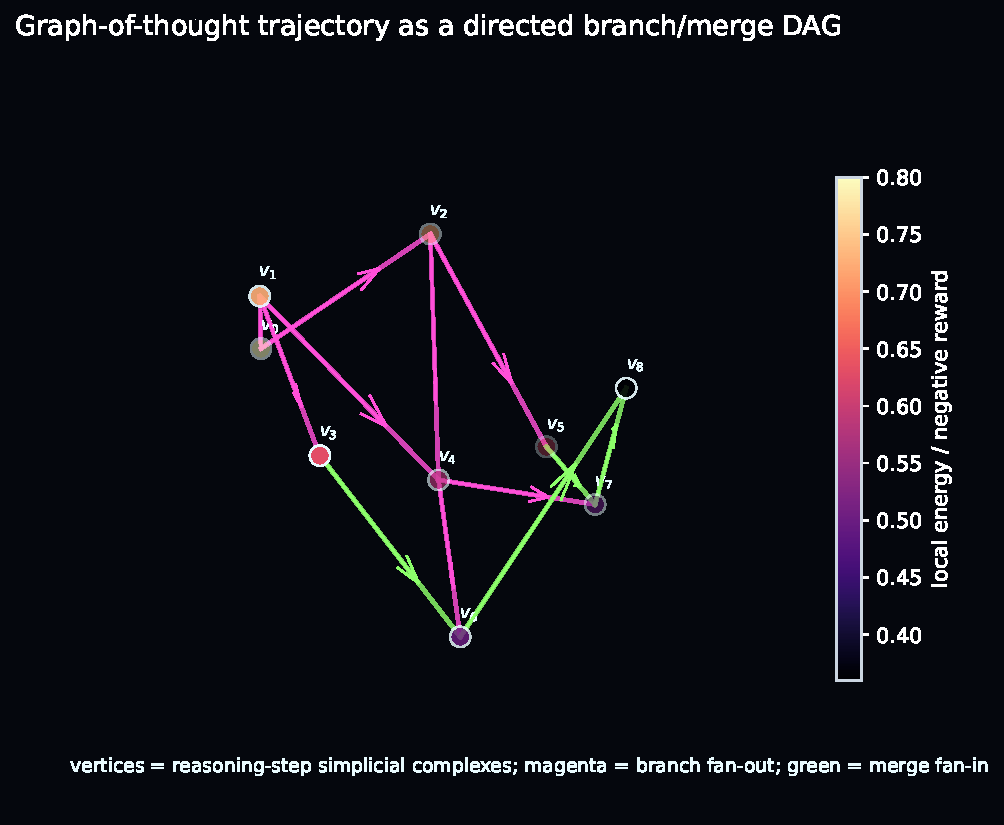
\includegraphics[width=0.92\textwidth]{fig_graph_of_thought_branch_merge_dag.pdf}
  \caption{Graph-of-thought trajectory as a directed branch/merge DAG.  Each vertex represents a reasoning-step simplicial complex with hidden state, behavior alcove, toric/tropical chamber, and certificate signature.  Branch fan-out explores alternatives; merge fan-in reconciles or selects them.}
  \label{fig:got-branch-merge-dag}
\end{figure}

The memory index is a graph $M=(V_M,E_M)$ whose vertices store $(h,\xi,C,A,\Delta,\Sigma_{\mathrm{TBGG}},q)$: hidden state, GraphCG coordinate, chamber, exponent table, complex, certificate signature, and verifier or BPB-derived quality.  Retrieval score becomes
\begin{equation}
  r(q,m)
  =
  \lambda_h\ip{\frac{h_q}{\norm{h_q}_2+\epsilon}}{\frac{h_m}{\norm{h_m}_2+\epsilon}}
  +\lambda_\Sigma\ip{\Sigma(q)}{\Sigma(m)}
  -\lambda_C\dist(S_{\pi,C_q}(\xi_q),K_{\pi,C_m})^2
  -\lambda_{\mathrm{bad}}\mathcal L_{\mathrm{SR}}^{\mathrm{beh}}(m).
\end{equation}
Analogical reasoning is accepted only when a source behavior corridor transports to the target corridor.  With a soft transport $P_{s\to t}$ and affine coordinate map $A_{s\to t}$, define
\begin{equation}
  \mathcal L_{\mathrm{analogy\text{-}corr}}
  =
  \norm{S_t(P_{s\to t}\xi_s)-A_{s\to t}S_s(\xi_s)}_2^2
  +\dist(S_t(P_{s\to t}\xi_s),K_{\pi,C_t})^2
  +\norm{\partial_tP_{s\to t}-P_{s\to t}\partial_s}_F^2 .
\end{equation}
This distinguishes helpful analogy from superficial mimicry: the analogy must preserve filtered topological structure and land in an acceptable behavior alcove.

\paragraph{Why the algebra can improve BPB and behavior.}
The BPB mechanism is indirect but testable.  Better GraphCG axes reduce superposition among byte-level concepts; corridor regularization prevents hidden trajectories from wasting capacity on unstable behavioral modes; Stanley--Reisner nonface penalties suppress incompatible feature coactivations; toric-binomial constraints make active chambers reusable across contexts; and resolution/DG losses make multi-step reasoning compositional.  These effects can lower conditional entropy when they make prefixes more predictable, but they must be subordinate to the base likelihood.  The correct training rule is therefore conservative: enable corridor metrics at analysis time, train them with micro weights, promote only those whose ablation improves BPB, verifier accuracy, memory retrieval, or out-of-distribution reasoning, and keep deployable artifacts free of any training-only certificate that does not improve the audited score.

\paragraph{Computable protocol.}
The implementation follows a finite recipe.
\begin{enumerate}[leftmargin=2em]
  \item Build contrastive behavior sets and learn GraphCG axes $B_q$; retain axes only if intervention and disentanglement audits pass.
  \item Fit chamberwise steering maps $S_{\pi,C}$ and corridors $K_{\pi,C}$ from helpful/unhelpful labels, verifier support, policy tags, and style/detail targets.
  \item Construct exact small certificates $(A,\Delta,I_A,F_\bullet,\mathrm{Fitt},\mathrm{DG})$ for sampled reasoning windows.
  \item Train with $\mathcal L_{\mathrm{BMP}}$ at BPB-safe weights and CE-ratio caps; log corridor distance, alcove occupancy, wall hits, SR nonface mass, toric-binomial residuals, Fitting jumps, Betti drift, DG residuals, memory compatibility, and analogy-corridor residuals.
  \item At inference, use \eqref{eq:bgg-behavior-projection} only when hidden states leave calibrated bands; otherwise leave the model untouched.
  \item Periodically materialize exact symbolic resolutions and topological objects in sidecar analyses to verify that differentiable metrics still correspond to the intended algebraic objects.
\end{enumerate}

\subsection{Losses used in training}

The full Toric BGG objective is a late-phase auxiliary objective, not a replacement for BPB or supervised graph losses.  With $H$ denoting hidden states and $\mathcal C$ the certificate, use
\begin{align}
  \mathcal L_{\mathrm{TBGG}}={}&
  \lambda_{\partial^2}\mathcal L_{\partial^2}
  +\lambda_D\mathcal L_D
  +\lambda_{\mathrm{std}}\mathrm{Leak}_{\mathrm{std}}
  +\lambda_{\mathrm{Kos}}\mathcal L_{\mathrm{Kos}}
  +\lambda_{\mathrm{Gale}}\mathcal L_{\mathrm{Gale}}\notag\\
  &+\lambda_{\mathrm{EK}}\mathcal L_{\mathrm{EulerKoszul}}
  +\lambda_{\mathrm{sig}}\mathcal L_{\mathrm{signature}}
  +\lambda_{\mathrm{pur}}(1-\mathrm{Pur}_{\mathcal O}).
\end{align}
The base training objective becomes
\begin{equation}
  \mathcal L=\mathcal L_{\mathrm{LM/BPB}}+\mathcal L_{\mathrm{graph}}+\mathcal L_{\mathrm{tropical}}+\mathcal L_{\mathrm{GFlowNet}}+\mathcal L_{\mathrm{GraphCG}}+\mathcal L_{\mathrm{TBGG}}.
\end{equation}
The scheduler must keep $\lambda_{\mathrm{TBGG}}$ effectively zero until the base model has learned stable byte and graph likelihood.  In practice, the first useful BGG loss is usually $\mathcal L_{\partial^2}$ because it is local and well-conditioned.  Gale-dual and Euler-Koszul losses are introduced only after the chain-map residual and standard leakage are already small on synthetic certificates.

\begin{definition}[Koszul-linearity residual]\label{def:koszul-residual}
Suppose a certificate gives a minimal graded resolution $P_\bullet\to L$ of a simple or residue module and the expected Koszul pattern is that generators in homological degree $k$ occur in internal degree $k+c$.  Let $\widehat w_{k,j}$ be the model's predicted mass for generators in homological degree $k$ and internal degree $j$.  Define
\begin{equation}
  \mathcal L_{\mathrm{Kos}}=\sum_{k,j}\widehat w_{k,j}\,\abs{j-k-c}.
\end{equation}
For non-Koszul certificates, the expected degree profile is replaced by the certificate's Betti table.
\end{definition}

\begin{definition}[Signature distillation loss]\label{def:signature-distillation}
Let $r_\psi(s,i)$ be the anticipative retrieval score for state $s$ and memory item $i$.  Let $\widetilde r(s,i)$ be the teacher score
\begin{equation}
  \widetilde r(s,i)=\alpha\ip{\Sigma_{\mathrm{TBGG}}(s)}{\Sigma_{\mathrm{TBGG}}(i)}+\beta\ip{\xi_s}{\xi_i}+\gamma q_i-\delta d_{\mathrm{top}}(s,i).
\end{equation}
The signature distillation loss is
\begin{equation}
  \mathcal L_{\mathrm{signature}}=\mathrm{KL}\bigl(\softmax(\widetilde r)\,\Vert\,\softmax(r_\psi)\bigr).
\end{equation}
It trains the memory head to retrieve helper trajectories that match both embedding geometry and finite resolution structure.
\end{definition}

\subsection{Why this can improve BPB}

BPB is a log score.  A structural auxiliary can improve BPB only if it changes the predictive distribution on future bytes or symbols.  The role of Toric BGG is to improve hidden-state organization so that the model assigns higher probability to continuations requiring algebraic, graph-theoretic, or analogical reasoning.  The following elementary bound is useful for evaluating mixture heads and retrieval-augmented predictions.

\begin{proposition}[Safe interpolation bound for BPB heads]\label{prop:bpb-mixture}
Let $q_0(\cdot\mid c)$ be a base next-byte distribution and $q_1(\cdot\mid c)$ a Toric-BGG-assisted distribution, both normalized.  For $\alpha\in[0,1)$ define
\begin{equation}
  q_\alpha=(1-\alpha)q_0+\alpha q_1.
\end{equation}
For every observed byte $b$,
\begin{equation}
  -\log_2 q_\alpha(b\mid c)\leq -\log_2 q_0(b\mid c)-\log_2(1-\alpha).
\end{equation}
Moreover, $q_\alpha$ improves the per-byte log score over $q_0$ exactly when
\begin{equation}
  \frac{q_1(b\mid c)}{q_0(b\mid c)}>1.
\end{equation}
The first-order improvement at $\alpha=0$ is
\begin{equation}
  \left.\frac{d}{d\alpha}\bigl[-\log_2 q_\alpha(b\mid c)\bigr]\right|_{\alpha=0}
  =-\frac{1}{\ln2}\left(\frac{q_1(b\mid c)}{q_0(b\mid c)}-1\right).
\end{equation}
\end{proposition}

\begin{proof}
Since $q_\alpha\geq(1-\alpha)q_0$, taking negative base-two logarithms gives the upper bound.  The mixture improves the log score exactly when $q_\alpha(b)>q_0(b)$, which for $\alpha>0$ is equivalent to $q_1(b)>q_0(b)$.  Differentiating $-\log_2((1-\alpha)q_0+\alpha q_1)$ at $\alpha=0$ gives the derivative.
\end{proof}

The practical implication is that a Toric-BGG head should be measured by conditional lift, not by aesthetic diagnostics.  The right metric is
\begin{equation}
  \Delta\mathrm{BPB}_{\mathrm{TBGG}}=\frac{1}{N}\sum_t\log_2\frac{q_{\mathrm{base}}(b_t\mid c_t)}{q_{\mathrm{TBGG}}(b_t\mid c_t)},
\end{equation}
reported globally and on tagged slices: algebraic normal-form text, graph-json continuations, proof steps, Hebrew morphology, and ordinary FineWeb prose.  If $\Delta\mathrm{BPB}_{\mathrm{TBGG}}$ is positive only on synthetic algebra and negative on natural text, the loss is not ready for the contest track.

\subsection{Train-time computation}

The following table lists the finite objects that can be computed during training.  The default implementation should cache the certificate and stream only compact tensors to the GPU.

\begin{longtable}{p{0.22\textwidth}p{0.28\textwidth}p{0.36\textwidth}}
\toprule
Object & CPU construction & GPU loss \\
\midrule
Sign-vector poset & enumerate covectors or sample feasible bounded sign vectors & standard-mask leakage, order prediction \\
Incidence proxy algebra & build sparse interval basis $e_{xy}$ & projective-factor labels, standard purity \\
BGG/Koszul complex & construct signed sparse boundary matrices & $\partial^2$ residual, differential alignment \\
Toric Tate strand & precompute strongly linear strand or Betti slice & degree-profile and linearity loss \\
Gale-dual pair & compute kernel matrix and matroid complements & dual-signature consistency \\
Euler-Koszul certificate & build commuting Euler operator matrices on a finite truncation & Koszul exactness and resonance classification \\
Trajectory signature & summarize hidden path after rollout & retrieval distillation, analogical helper ranking \\
Variety-of-complexes stratum & fix Betti format $b$ and rank sequence $r$, then audit $d^2=0$ and rank minors & chain-composition residual, soft-rank stratum loss, degeneration-order barrier \\
Fitting/BE exactness audit & compute presentation minors, Fitting ideals, and Buchsbaum--Eisenbud complementary multipliers & differentiable minor residuals and exactness alarms for sidecar promotion \\
Derived comparator & build chain maps and mapping cones between two certificate complexes & analogy loss, memory-similarity score, quasi-isomorphism or degeneration distance \\
\bottomrule
\end{longtable}

A minimal implementation has this interface.
\begin{verbatim}
@dataclass
class ToricBGGCertificate:
    poset_cover_edges: LongTensor       # [num_edges, 2]
    standard_mask: BoolTensor           # [m, m]
    boundary: list[SparseTensor]        # D_k: C_k -> C_{k-1}
    internal_degree: LongTensor         # basis-element degree labels
    betti_target: FloatTensor           # flattened Betti or homology profile
    gale_partner_id: Optional[str]
    euler_koszul: Optional[list[SparseTensor]]
    metadata: dict

class ToricBGGProbe(nn.Module):
    def forward(self, hidden, cert):
        D_hat = predict_boundaries(hidden, cert)
        std_logits = predict_standard_labels(hidden, cert)
        signature = summarize_resolution(hidden, D_hat, cert)
        return D_hat, std_logits, signature
\end{verbatim}
The boundary matrices should be sparse and batch-local.  For a 128-basis certificate, the $\partial^2$ loss is negligible compared with attention.  The expensive work is certificate generation, which should be cached by hash.

\subsection{Integration with the existing architecture}

The Toric BGG layer enters ToricGT at five points.

\paragraph{Tropical heads.}
Tropical attention already computes exposed faces of Newton polytopes.  BGG certificates add labels to those faces: a face can be a standard object, a cover relation, a monomial generator, or a differential term.  The active-face margin becomes a confidence score for a step in a resolution.

\paragraph{GraphCG axes.}
GraphCG supplies a disentangled coordinate chart.  Toric BGG supervision asks some axes to correspond to standard directions: moving along an axis should change a controlled standard label, internal degree, or Gale-dual coordinate rather than globally perturbing all hidden features.  This is measured by standard purity and pullback fan sharpness.

\paragraph{Analogical trajectory memory.}
The memory head should retrieve helper trajectories that match both semantic embedding and resolution signature.  Two proofs with the same homological skeleton but different surface tokens are better analogical helpers than two proofs with nearby final embeddings but incompatible complexes.

\paragraph{Soft-MoE routing.}
The typed expert bank gains a BGG/resolution expert.  Its function is small: predict boundary terms, standard labels, and signature vectors.  Under a byte cap, this expert should be a low-rank adapter sharing the dense MLP, not a full separate MLP.

\paragraph{Parameter-Golf BPB training.}
The exported micro-LM should not store a large algebraic module.  It may store compact phase features, recurrent weights, and perhaps an int8 low-rank BGG probe if and only if ablations show a net BPB gain.  Otherwise the BGG layer is training-only, used for distillation and checkpoint selection.

\begin{figure}[t]
  \centering
  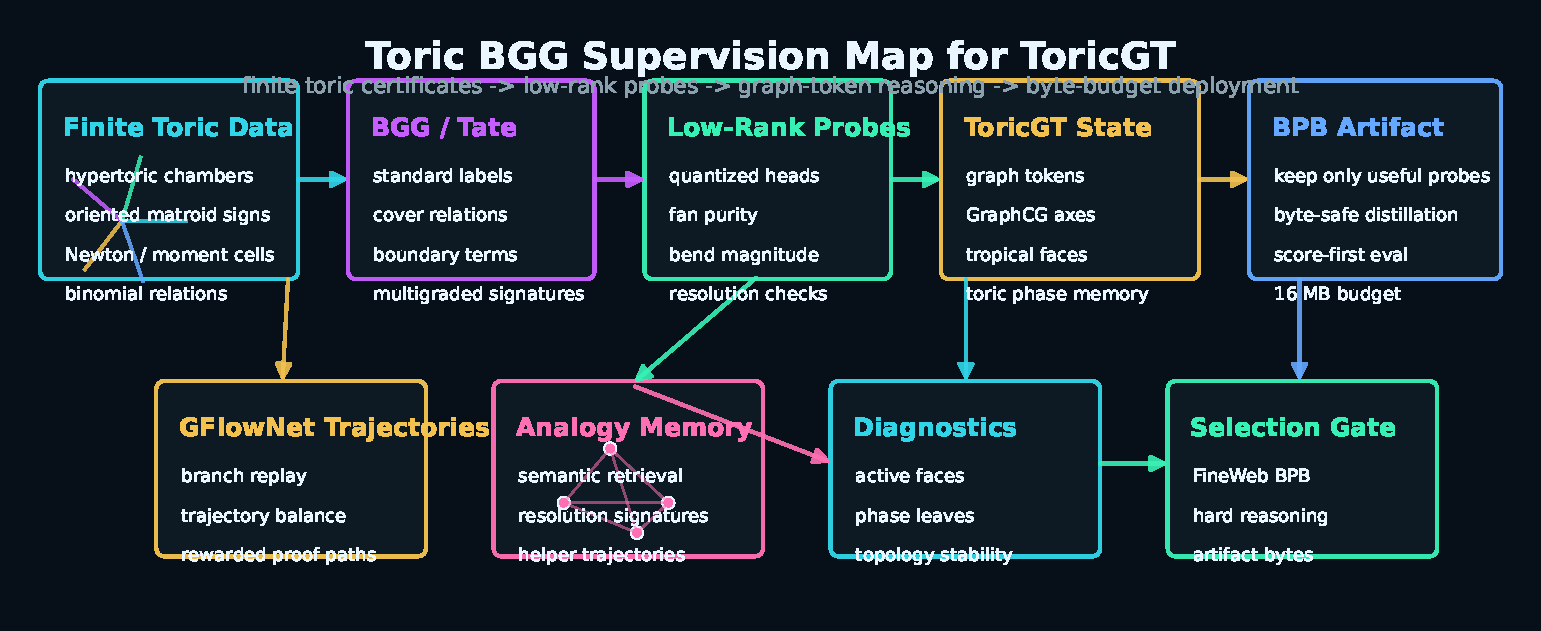
\includegraphics[width=\textwidth]{fig_toric_bgg_training_map.pdf}
  \caption{Toric BGG supervision for ToricGT.  Hypertoric arrangements, oriented matroids, and multigraded BGG/Tate resolutions generate finite certificates.  Low-rank probes attach those certificates to graph-token hidden states, GraphCG concept axes, GFlowNet trajectories, and retrieval memory.  The deployable BPB model keeps only components that improve validation log score under the artifact budget.}
  \label{fig:toric-bgg-map}
\end{figure}

\subsection{Metrics}

Toric BGG training should be judged by a small set of metrics that are hard to game.

\begin{definition}[Toric BGG evaluation metrics]\label{def:tbg-metrics}
For an evaluation run, report:
\begin{align}
  \mathrm{RCS} &= 1-\frac{\sum_k\norm{\widehat D_{k-1}\widehat D_k}_F}{\sum_k\norm{\widehat D_k}_F+\epsilon}, &&\text{resolution consistency,}\\
  \mathrm{SFL} &= \frac{1}{|\Lambda|}\sum_\lambda\sum_{\mu\not\leq\lambda}\mathrm{Attn}_{\lambda\mu}, &&\text{standard-filtration leakage,}\\
  \mathrm{KLR} &= \sum_{k,j}\widehat w_{k,j}\abs{j-k-c}, &&\text{Koszul-linearity residual,}\\
  \mathrm{GDC} &= \norm{G_\theta s_A-s_B}_2, &&\text{Gale-dual consistency,}\\
  \mathrm{BTR@}K &= \Pr[\text{useful helper appears in top }K\text{ memory hits}], &&\text{BGG trajectory retrieval,}\\
  \Delta\mathrm{BPB}_{\mathrm{TBGG}} &= \frac{1}{N}\sum_t\log_2\frac{q_{\mathrm{base}}(b_t\mid c_t)}{q_{\mathrm{TBGG}}(b_t\mid c_t)}, &&\text{log-score lift.}
\end{align}
\end{definition}

The first five metrics certify structure.  The last metric decides whether the structure helps compression and predictive modeling.  A model with attractive RCS or GDC but negative $\Delta\mathrm{BPB}_{\mathrm{TBGG}}$ is not a better Parameter-Golf model.  It may still be a better graph-reasoning model if held-out proof and algebra tasks improve.

\subsection{A staged training protocol}

The safest protocol is sequential.

\begin{enumerate}[leftmargin=2em]
  \item \textbf{Audit-only pass.}  Run the current checkpoint on toric, hypertoric, graph, and natural-text slices.  Compute RCS, SFL, KLR, GDC, BTR@$K$, and $\Delta\mathrm{BPB}$ with probes frozen or absent.  This establishes the baseline geometry.
  \item \textbf{Probe-only training.}  Freeze the encoder.  Train low-rank BGG probes to predict boundary matrices, standard labels, and signatures.  If probe accuracy is poor, the representation does not yet contain the required structure; do not unfreeze the model.
  \item \textbf{Adapter fine-tuning.}  Unfreeze only upper-layer adapters, Soft-MoE low-rank deltas, and retrieval heads.  Use $\mathcal L_{\partial^2}$, standard leakage, and signature distillation.  Keep Gale-dual and Euler-Koszul weights at zero.
  \item \textbf{Duality phase.}  Introduce Gale-dual pairs and Euler-Koszul certificates on synthetic and curated algebra slices.  Stop if ordinary validation BPB worsens beyond the predeclared tolerance.
  \item \textbf{Distillation and export.}  Distill any improvement into the micro-LM.  Export from the serialized artifact and re-evaluate.  A floating-point checkpoint improvement is not sufficient.
\end{enumerate}

This protocol is compatible with the existing ToricGT training program.  It does not detract from tropical attention, noncommutative phase memory, GraphCG, GFlowNet, Hebrew morphology, Soft-MoE, or Parameter-Golf compression.  It gives those components a finite algebraic contract: when the data contain a resolution, the hidden trajectory should behave like one.


\section{Rotation algebras, noncommutative tori, and spiral projections}

\subsection{Finite Weyl pairs and normal forms}

For $\theta\in\R$, the rotation algebra $\A_\theta$ is generated by unitaries $U,V$ satisfying
\begin{equation}
  VU=e^{2\pi i\theta}UV.
\end{equation}
For rational $\theta=p/q$, finite clock and shift matrices give an exact Weyl pair.  Let $\omega=e^{2\pi i p/q}$,
\begin{equation}
  C_q=\diag(1,\omega,\omega^2,\ldots,\omega^{q-1}),\qquad S_q e_j=e_{j-1\bmod q}.
\end{equation}

\begin{lemma}[Finite clock-shift relation]
The matrices $S_q$ and $C_q$ satisfy
\begin{equation}
  S_qC_q=\omega C_qS_q.
\end{equation}
\end{lemma}

\begin{proof}
Apply both sides to a basis vector $e_j$, with indices interpreted modulo $q$.  Since $C_qe_j=\omega^j e_j$ and $S_qe_j=e_{j-1}$,
\begin{equation}
  S_qC_qe_j=\omega^j e_{j-1}.
\end{equation}
On the other hand,
\begin{equation}
  \omega C_qS_qe_j=\omega C_qe_{j-1}=\omega\cdot\omega^{j-1}e_{j-1}=\omega^j e_{j-1}.
\end{equation}
The two operators agree on every basis vector, so $S_qC_q=\omega C_qS_q$.
\end{proof}

\begin{remark}[Convention discipline]
The sign of the clock-shift phase is a common source of synthetic-data bugs.  Every generated record must store the shift convention, the normal-form order, and whether the relation is $VU=\omega UV$ or $UV=\omega VU$.
\end{remark}

\begin{lemma}[Rotation-word normal form]
Let $VU=\omega UV$, where $\omega=e^{2\pi i\theta}$.  Every word in $U^{\pm1},V^{\pm1}$ reduces to a unique expression
\begin{equation}
  \omega^c U^aV^b,
\end{equation}
where $a,b,c\in\Z$, after fixing the normal-form order $U$ before $V$.  If the word is $W=X_1\cdots X_T$ and $\deg(X_t)=(u_t,v_t)\in\Z^2$, then
\begin{equation}
  a=\sum_{t=1}^T u_t,
  \qquad b=\sum_{t=1}^T v_t,
  \qquad c=\sum_{1\le r<s\le T} v_r u_s,
\end{equation}
with signs interpreted by the same commutation convention.
\end{lemma}

\begin{proof}
The relation $VU=\omega UV$ allows any adjacent out-of-order pair $VU$ to be swapped into $UV$ at the cost of multiplying by $\omega$.  Similarly, inverse pairs cancel using $UU^{-1}=U^{-1}U=VV^{-1}=V^{-1}V=1$, and inverse commutations follow by multiplying the basic relation by inverses.  Repeated adjacent swaps bubble all $U$ powers to the left and all $V$ powers to the right.  The net exponents $a$ and $b$ are additive because $U$ and $V$ powers combine within their own generators.  The phase exponent counts signed crossings in which a $V$ contribution originally appears before a later $U$ contribution; this is exactly $\sum_{r<s}v_ru_s$.  Confluence follows because this crossing count depends only on the ordered degree sequence, and all swap sequences that sort the word have the same inversion count in the abelianized degree lattice with the same bilinear cocycle.
\end{proof}

\subsection{Higher noncommutative tori}

A higher noncommutative torus $\A_\Theta$ is generated by $U_1,\ldots,U_n$ with
\begin{equation}
  U_jU_k=e^{2\pi i\Theta_{jk}}U_kU_j,
\end{equation}
where $\Theta\in\R^{n\times n}$ is skew-symmetric.  For $a,b\in\Z^n$, define the cocycle
\begin{equation}
  \sigma_\Theta(a,b)=\exp(2\pi i a\transpose\Theta b).
\end{equation}

\begin{lemma}[Bicharacter identities]
For $a,b,c\in\Z^n$,
\begin{align}
  \sigma_\Theta(a+b,c)&=\sigma_\Theta(a,c)\sigma_\Theta(b,c),\\
  \sigma_\Theta(a,b+c)&=\sigma_\Theta(a,b)\sigma_\Theta(a,c),\\
  \sigma_\Theta(a,b)\sigma_\Theta(b,a)&=1.
\end{align}
\end{lemma}

\begin{proof}
The first two identities follow from bilinearity:
\begin{equation}
  (a+b)\transpose\Theta c=a\transpose\Theta c+b\transpose\Theta c,
\end{equation}
and similarly in the second argument.  Exponentiating turns sums into products.  For the third identity, skew-symmetry gives $b\transpose\Theta a=-a\transpose\Theta b$.  Hence the exponents sum to zero.
\end{proof}

\begin{proposition}[Projective equivariance of toric transports]
Let $T_a$ be a lattice transport on toric channels satisfying
\begin{equation}
  T_aT_b=\sigma_\Theta(a,b)T_{a+b}.
\end{equation}
If token relabelings act on rows and $T_a$ acts only on toric feature channels attached equivariantly to each row, then ToricGT layers built from shared maps, attention, and $T_a$ are graph-equivariant and projectively lattice-equivariant.
\end{proposition}

\begin{proof}
A graph relabeling $P_\pi$ acts by row permutation.  A toric transport $T_a$ acts within the channel vector of every row by the same linear operator or by an endpoint-derived equivariant channel rule.  Therefore $P_\pi T_a=T_aP_\pi$.  The only noncommutativity among transports is the scalar cocycle $\sigma_\Theta(a,b)$, which yields projective equivariance.  Since all other sublayers are row-shared and equivariant, the composition retains graph equivariance and the stated projective lattice law.
\end{proof}

\subsection{Infinite spiral projection}

The infinite spiral view is a visualization, not a finite representation theorem.  It makes the irrational rotation visible: repeated additions of $\alpha$ never close when $\alpha$ is irrational, and the orbit winds densely.

\begin{lemma}[Density of an irrational circle orbit]
If $\alpha\notin\Q$, then the set $\{k\alpha\bmod 1:k\in\N\}$ is dense in $[0,1)$.
\end{lemma}

\begin{proof}
Fix $N\in\N$.  Consider the $N+1$ points $0,\alpha,2\alpha,\ldots,N\alpha$ modulo $1$.  Partition $[0,1)$ into $N$ intervals of length $1/N$.  By the pigeonhole principle, two points $r\alpha$ and $s\alpha$ lie in the same interval, so $\delta=(s-r)\alpha\bmod 1$ has distance at most $1/N$ from $0$.  Since $\alpha$ is irrational, $\delta\ne0$.  The arithmetic progression $0,\delta,2\delta,\ldots$ modulo $1$ visits every interval of length roughly $1/N$ before wrapping.  Because $N$ was arbitrary, every open interval contains some $k\alpha\bmod1$.
\end{proof}

\begin{definition}[Spiral projection feature]
For irrational $\alpha$ and truncation length $K$, define the spiral-projection feature path
\begin{equation}
  \Gamma_K(k)=\left(\cos(2\pi k\alpha),\sin(2\pi k\alpha),k/K\right),\qquad 0\le k<K,
\end{equation}
and the projected torus path
\begin{equation}
  \Pi_K(k)=\left((R+r\cos(2\pi k\beta))\cos(2\pi k\alpha),
  (R+r\cos(2\pi k\beta))\sin(2\pi k\alpha),
  r\sin(2\pi k\beta)\right),
\end{equation}
where $1,\alpha,\beta$ are rationally independent.
\end{definition}

\begin{figure}[t]
  \centering
  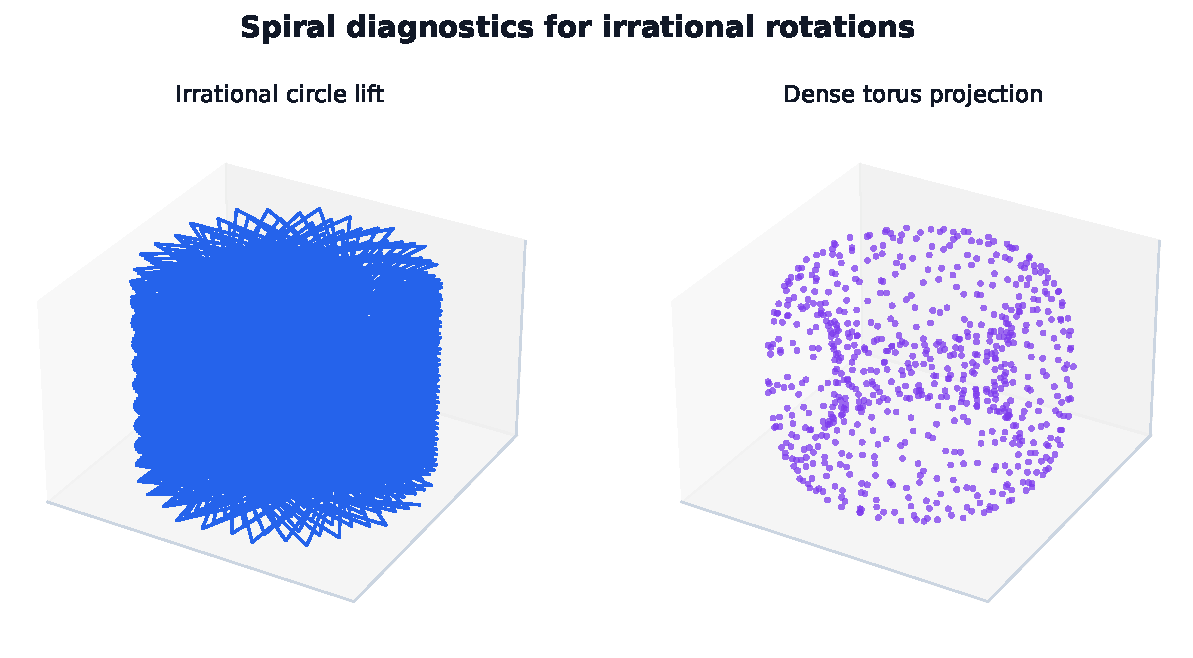
\includegraphics[width=0.92\textwidth]{fig_spiral_projection.pdf}
  \caption{Infinite spiral-projection diagnostic for the rotation algebra and noncommutative torus.  The cylinder shows irrational rotation by $\alpha$; the torus projection visualizes dense phase winding and finite phase-channel truncations.}
  \label{fig:spiral}
\end{figure}

\begin{proposition}[Finite feature convergence of phases]
Let $p_k/q_k$ be continued-fraction approximants to $\alpha$.  Then
\begin{equation}
  \abs{e^{2\pi i p_k/q_k}-e^{2\pi i\alpha}}\le 2\pi\abs{p_k/q_k-\alpha}\to0.
\end{equation}
\end{proposition}

\begin{proof}
For real $x,y$, $\abs{e^{ix}-e^{iy}}=2\abs{\sin((x-y)/2)}\le\abs{x-y}$.  Set $x=2\pi p_k/q_k$ and $y=2\pi\alpha$.  Continued-fraction convergence gives $p_k/q_k\to\alpha$.
\end{proof}

\subsection{Trace supervision}

The canonical trace on the rotation algebra satisfies
\begin{equation}
  \tau(U^aV^b)=\begin{cases}1,&a=b=0,\\0,&\text{otherwise.}\end{cases}
\end{equation}
For a finite Weyl-pair approximation, the normalized trace $q^{-1}\Tr(C_q^aS_q^b)$ obeys the same selection rule modulo $q$.

\begin{lemma}[Finite trace selection]
For the $q$-dimensional Weyl pair, if $a,b\in\Z$, then
\begin{equation}
  \frac1q\Tr(C_q^aS_q^b)=0
\end{equation}
unless $a\equiv b\equiv0\pmod q$, in which case the normalized trace is $1$.
\end{lemma}

\begin{proof}
If $b\not\equiv0\pmod q$, then $S_q^b$ has no fixed basis vector, so $C_q^aS_q^b$ has zero diagonal and zero trace.  If $b\equiv0\pmod q$, then $S_q^b=I$ and
\begin{equation}
  \Tr(C_q^a)=\sum_{j=0}^{q-1}\omega^{aj}.
\end{equation}
This geometric sum is $q$ when $\omega^a=1$, equivalently $a\equiv0\pmod q$, and is $0$ otherwise.
\end{proof}

\section{Hebrew roots as graph-structured morphology}

\subsection{Why Hebrew morphology belongs in ToricGT}

Biblical and classical Hebrew morphology is naturally graph-structured.  A surface form is not merely a string: it is related to a lexical root, ordered radicals, a vocalic/consonantal template, a binyan or stem, prefixes and suffixes, morphosyntactic features, a lemma, a gloss, and a source span.  These objects form a typed graph with many-to-many dependencies.  A root such as \heb{כתב} (transliterated K-T-B) participates in forms such as \emph{katav} (\heb{כָּתַב}, ``he wrote''), \emph{kotev} (writing/writer), and \emph{miktav} (letter or writing).  A model trained only on linear strings must rediscover this structured factorization; a graph-token model can represent it explicitly.

Classical grammars describe Hebrew and other Semitic languages through roots, stems, and patterns; computational morphology often implements such analyses with finite-state or two-level systems \cite{gesenius1910,waltke1990,joüon2006,koskenniemi1983,beesley2003,yona2008}.  ToricGT does not replace a morphological analyzer.  It consumes analyzer outputs, text spans, and uncertain analyses as typed graph evidence, and learns graph-to-graph tasks over those analyses.

\begin{definition}[Hebrew root-template record]
A Hebrew morphology record is a typed graph
\begin{equation}
  G_H=(V_H,E_H,\tau,\rho,x,\ell,y)
\end{equation}
with node types
\begin{equation}
\begin{split}
  \mathcal T_V^H=\{&\Root,\mathsf{Radical},\Pat,\Binyan,\Feat,\mathsf{Prefix},\mathsf{Suffix},\\
  &\mathsf{SurfaceForm},\mathsf{Lemma},\mathsf{Gloss},\mathsf{VerseSpan},\mathsf{Paradigm},\mathsf{AnalyzerHypothesis}\},
\end{split}
\end{equation}
and edge types
\begin{equation}
\begin{split}
  \mathcal T_E^H=\{&\mathsf{has\_radical},\mathsf{fills\_slot},\mathsf{has\_template},\mathsf{has\_binyan},\mathsf{has\_feature},\\
  &\mathsf{attested\_at},\mathsf{glosses},\mathsf{same\_root},\mathsf{paradigm\_member},\mathsf{analyzer\_score}\}.
\end{split}
\end{equation}
The target $y$ may include root identity, radical-slot alignment, binyan, feature bundle, lemma, gloss, paradigm membership, and confidence.
\end{definition}

\begin{figure}[t]
  \centering
  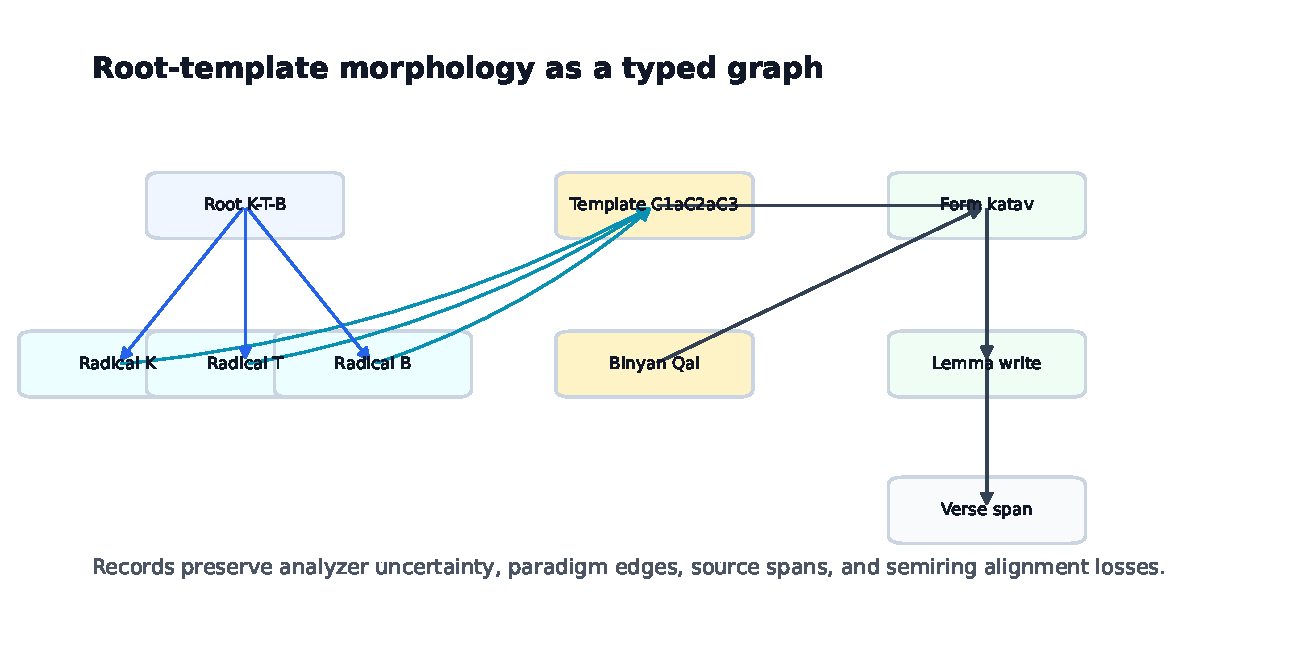
\includegraphics[width=\textwidth]{fig_hebrew_root_graph.pdf}
  \caption{A root-template graph for K-T-B.  The actual graph record can also store Hebrew glyphs and source spans; the figure uses transliteration for directional readability.}
  \label{fig:hebrew-root}
\end{figure}

\begin{definition}[Root-template rendering relation]
Let $r=(r_1,r_2,r_3)$ be an ordered radical tuple, $p$ a template with consonant slots $C_1,C_2,C_3$ and vocalic/affix material, $b$ a binyan, and $f$ a feature bundle.  The rendering relation is a partial relation
\begin{equation}
  \mathcal R_H\subseteq \Root\times\Pat\times\Binyan\times\Feat\times\mathsf{SurfaceForm}
\end{equation}
where $(r,p,b,f,w)\in\mathcal R_H$ if $w$ is licensed by inserting radicals into template slots and applying the orthographic/phonological rules attached to $b$ and $f$.
\end{definition}

\begin{remark}[Root ambiguity]
A Hebrew surface string can have multiple analyses.  Matres lectionis, missing niqqud, weak roots, gutturals, homographs, and clitic morphology can all create ambiguity.  The graph schema therefore allows multiple analyzer-hypothesis nodes with scores, instead of forcing a single gold analysis when the evidence is uncertain.
\end{remark}

\subsection{Graph construction algorithm}

Given a tokenized Hebrew or biblical-Hebrew text with optional morphology, construct $G_H$ as follows.
\begin{enumerate}[leftmargin=2em]
  \item Create one \texttt{SurfaceForm} node per token or morpheme span.
  \item For each analyzer hypothesis, create a hypothesis node with score $s_h$.
  \item Attach root, radical, template, binyan, feature, lemma, gloss, and span nodes.  Share root and paradigm nodes across forms when the analyzer or lexicon identifies the same root.
  \item Add \texttt{fills\_slot} edges from radicals to template slots and from slots to surface spans.
  \item Add \texttt{same\_root} and \texttt{paradigm\_member} edges between lexemes/forms with the same root family.
  \item Preserve uncertainty by edge weights or hypothesis scores rather than deleting non-maximal analyses.
\end{enumerate}

\begin{lemma}[Typed acyclicity of local morphology subgraphs]
If paradigm-sharing edges are removed, each local root-template analysis graph is acyclic when edges are oriented from abstract causes to surface evidence.
\end{lemma}

\begin{proof}
Order node types by the partial order
\begin{equation}
  \Root,\mathsf{Radical},\Pat,\Binyan,\Feat
  \prec \mathsf{AnalyzerHypothesis}\prec \mathsf{SurfaceForm}\prec \mathsf{Lemma},\mathsf{Gloss},\mathsf{VerseSpan}.
\end{equation}
Edges in a local analysis go from an earlier type to a later type, or from a hypothesis to a surface node.  Since every directed edge increases this type rank, no directed cycle can occur.  Paradigm-sharing edges intentionally introduce global family structure and are excluded from the local acyclicity claim.
\end{proof}

\begin{lemma}[Functoriality under graph relabeling]
Let $C$ be a deterministic converter from morphology records to typed graphs, and let $\pi$ be a relabeling of source token identifiers that preserves source spans and analyzer hypotheses.  Then
\begin{equation}
  C(\pi\cdot R)=\pi\cdot C(R).
\end{equation}
\end{lemma}

\begin{proof}
The converter creates graph nodes by deterministic functions of record fields: token id, span id, root id, hypothesis id, feature id, and lexicon id.  Relabeling source token ids simply relabels the nodes whose keys contain those token ids.  Shared lexical nodes such as root and binyan nodes are unaffected except for incident edge endpoints.  Therefore every node and edge in $C(R)$ is carried to the corresponding node and edge in $C(\pi R)$.
\end{proof}

\subsection{Hebrew morphology losses}

Let $p_R$, $p_B$, $p_F$, and $p_L$ denote predicted distributions over roots, binyanim, feature bundles, and lemmas.  Let $A\in[0,1]^{3\times S}$ be a predicted radical-to-slot alignment for a three-radical root and $A^\star$ the target alignment.  Define
\begin{align}
  \mathcal L_{\mathrm{root}} &= -\log p_R(R^\star),\\
  \mathcal L_{\mathrm{binyan}} &= -\log p_B(B^\star),\\
  \mathcal L_{\mathrm{feat}} &= -\sum_{f\in\mathcal F}\left[y_f\log p_F(f)+(1-y_f)\log(1-p_F(f))\right],\\
  \mathcal L_{\mathrm{align}} &= -\sum_{i=1}^3\sum_{s=1}^S A^\star_{is}\log A_{is}.
\end{align}
Paradigm consistency can be enforced by a cycle loss.  If $z_w$ is the embedding of a surface form and $z_R$ is the embedding of its root family,
\begin{equation}
  \mathcal L_{\mathrm{par}}=\sum_{(w,w'):\Root(w)=\Root(w')}\norm{(z_w-z_R)-(z_{w'}-z_R)}_2^2
  -\sum_{(w,u):\Root(w)\ne\Root(u)}\max(0,\gamma-\norm{z_w-z_u})^2.
\end{equation}

\begin{proposition}[Paradigm loss is relabeling invariant]
If root-family membership is represented by equivariant graph edges and embeddings transform by token permutation, then $\mathcal L_{\mathrm{par}}$ is invariant under graph relabeling.
\end{proposition}

\begin{proof}
Relabeling permutes the set of surface-form nodes and root-family edges but does not change which unordered pairs are same-root or different-root.  The summands depend only on Euclidean distances between the corresponding permuted embeddings.  Euclidean distance is unchanged by row reindexing.  Therefore the entire sum is invariant.
\end{proof}

\subsection{Tropical alignment for root extraction}

Root-template alignment can be cast as a shortest-path problem over a small weighted finite-state graph.  Let $w_1,\ldots,w_T$ be surface characters or consonantal skeleton symbols, and let template states record how many radical slots have been filled.  A transition either consumes a surface symbol as affix/vowel material or aligns it to the next radical slot.  With costs $c_t(q,q')$, the best analysis is
\begin{equation}
  D_{t+1}(q')=\min_q\left(D_t(q)+c_t(q,q')\right).
\end{equation}

\begin{theorem}[Root-template alignment is min-plus dynamic programming]
For a fixed finite template inventory and bounded token length $T$, the best radical-slot alignment is computed by a finite min-plus circuit and can therefore be represented by tropical ToricGT layers.
\end{theorem}

\begin{proof}
The dynamic program has finitely many states because the template inventory and maximum word length are bounded.  Each update is a minimum over finitely many predecessor states of an affine expression $D_t(q)+c_t(q,q')$.  This is a min-plus gate.  Unrolling for $T$ time steps yields a finite min-plus circuit.  By the tropical semiring approximation theorem above, ToricGT can implement or approximate this circuit on the bounded domain.
\end{proof}

\subsection{Hebrew graph tasks}

ToricGT should include at least the following Hebrew-specific tasks.
\begin{enumerate}[leftmargin=2em]
  \item \textbf{Root recovery}: predict the root node and ordered radicals from a surface form and context.
  \item \textbf{Binyan classification}: predict stem/binyan and verbal pattern.
  \item \textbf{Feature tagging}: predict person, number, gender, tense/aspect, state, and part of speech when represented in the source annotation.
  \item \textbf{Paradigm completion}: given several forms in a root family, predict missing forms or missing feature nodes.
  \item \textbf{Graph disambiguation}: choose among analyzer hypotheses using local context and source-span dependencies.
  \item \textbf{Interlinear graph construction}: convert text plus morphology into lemma, gloss, and dependency graphs.
\end{enumerate}

\section{Reasoning capacity and visualization contract}

\begin{figure}[t]
  \centering
  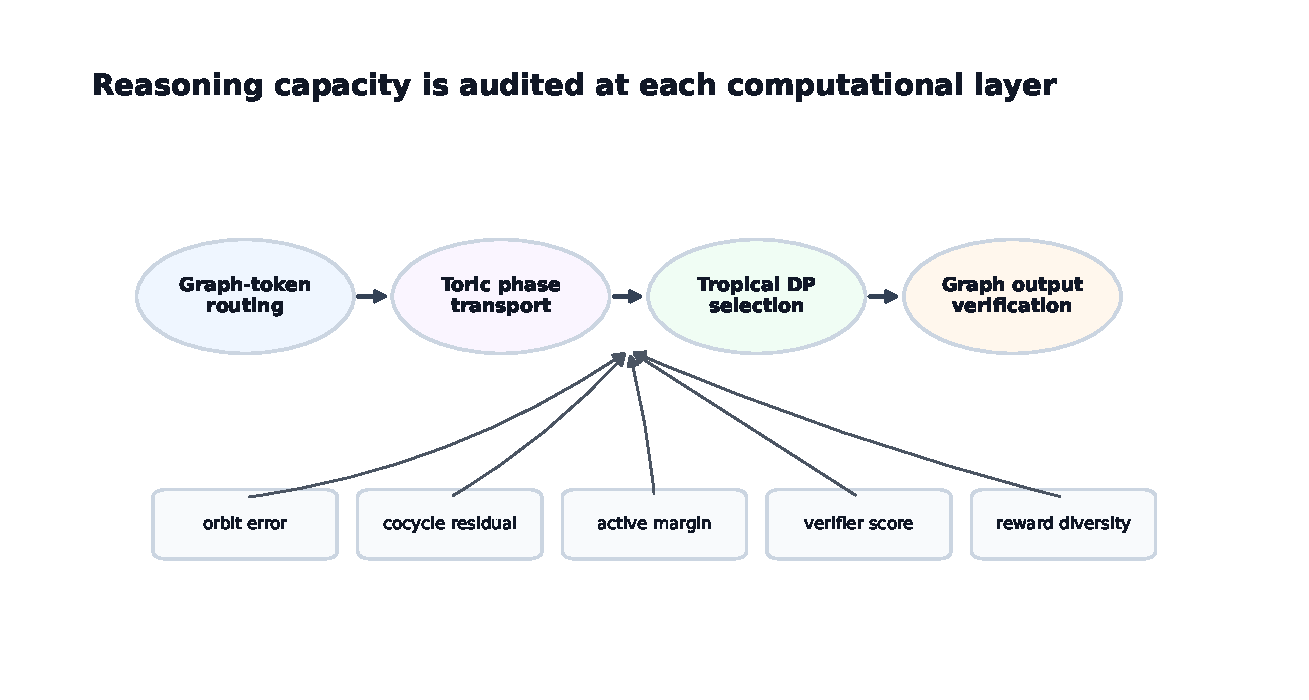
\includegraphics[width=\textwidth]{fig_reasoning_capacity.pdf}
  \caption{Reasoning capacity as a composition of graph-token routing, algebraic transport, tropical inference, and graph-level output.  The model should expose checks at each stage rather than returning only an answer string.}
  \label{fig:reasoning-capacity}
\end{figure}

\begin{definition}[Visualization contract]
A ToricGT run satisfies the visualization contract if it emits, for every evaluation batch, the following diagnostic objects: relabeling orbits, attention/ring block provenance, tropical active-face maps, toric phase trajectories, Hebrew root-template subgraphs when applicable, proof-dependency graphs, GFlowNet terminal samples, and reward/margin/error summaries.
\end{definition}

\begin{longtable}{p{0.23\linewidth}p{0.32\linewidth}p{0.34\linewidth}}
\toprule
Diagnostic & Computation & Failure mode exposed \\
\midrule
\endhead
Equivariance orbit & $\norm{F(\pi G)-P_\pi F(G)}$ over random $\pi$ & absolute-position leakage, edge-order bugs \\
Tropical active face & $A_{ic}=\argmax_j(S_{ij}+V_{jc})$ and margin $\Delta_{ic}$ & tropical collapse, unstable DP decisions \\
Torus commutator & $\norm{U_jU_kH-e^{2\pi i\Theta_{jk}}U_kU_jH}$ & phase memorization without cocycle structure \\
Hebrew paradigm lattice & root-family edges and feature-bundle consistency & string memorization without root-template abstraction \\
GFlowNet diversity & terminal graph count, edit distance, reward histogram & mode collapse, reward hacking \\
Polar cache residual & $\norm{K-\widehat K}$, $\norm{V-\widehat V}$, argmax preservation rate & quantization damaging long-context retrieval \\
\bottomrule
\end{longtable}

\begin{figure}[t]
  \centering
  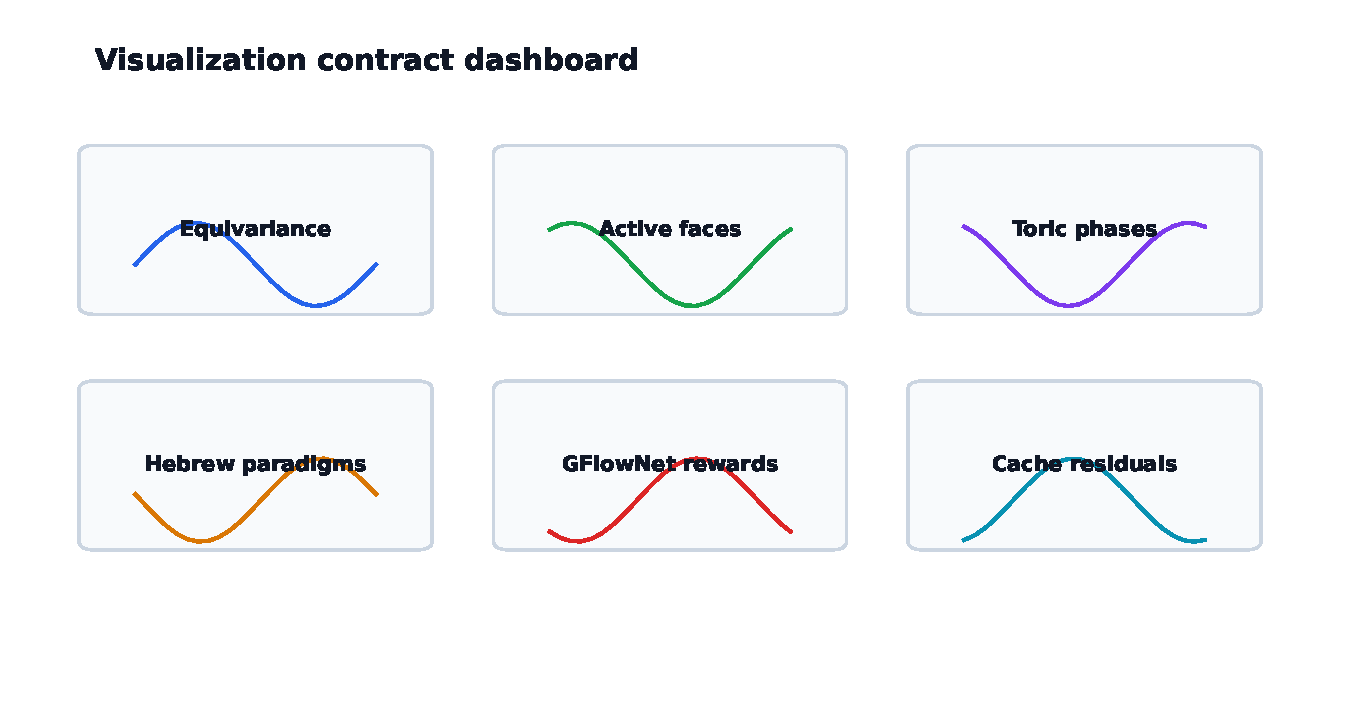
\includegraphics[width=\textwidth]{fig_visualization_dashboard.pdf}
  \caption{Visualization dashboard targets.  The dashboard should make reasoning behavior falsifiable: a good scalar metric is not sufficient if equivariance, phase, active-face, morphology, or diversity diagnostics fail.}
  \label{fig:viz-dashboard}
\end{figure}

The analysis suite implements this contract with interactive 3D diagnostics.  For each sampled graph-of-thought branch it plots focused hidden-state coordinates, local Vietoris--Rips 1/2-complexes, toric active-face colors, chamber-crossing markers, empirical normal-fan rays, convex chamber-polytopes for occupied active faces, fitted wall sheets at observed tropical/toric crossings, and a small Newton-polytope shadow built from the pseudo-exponents used by the empirical fan audit.  The energy-landscape companion lifts local NLL to the vertical axis and overlays the same chamber and wall geometry.  Sparse/default/dense controls adjust the local simplicial radius; Plotly legend toggles isolate branches, complexes, chambers, walls, and polytopes.

\begin{proposition}[Visualization invariance]
Suppose diagnostic functions are defined from graph-invariant quantities or equivariant token quantities followed by canonical graph rendering.  Then relabeling the input graph changes only node/edge labels in the visualization, not the diagnostic values.
\end{proposition}

\begin{proof}
Equivariance errors are norms of aligned outputs and are invariant under row permutation.  Active-face sets transform by the same token permutation, and canonical rendering quotients out token labels.  Commutator losses act on channel operators shared across rows, so row permutations do not change Frobenius norms.  Root-family and paradigm diagnostics are computed over graph edges whose incidence is preserved by relabeling.  GFlowNet terminal graph diversity is computed up to graph edit distance or canonical graph hashes.  Therefore the diagnostic values are invariant, while rendered node names may change.
\end{proof}

\section{Embedding-space GFlowNet fine-tuning}

A GFlowNet samples terminal graph objects with probability proportional to reward.  In ToricGT, the default Markov decision process acts in embedding space.

\begin{definition}[Embedding-space state]
A state is
\begin{equation}
  s_t=(h_G^{(t)},H_V^{(t)},H_E^{(t)},m^{(t)}),
\end{equation}
where $h_G$ is a graph embedding, $H_V$ and $H_E$ are node and edge latent tables, and $m$ is metadata such as current root-analysis hypotheses, proof obligations, braid word state, or torus normal-form state.
\end{definition}

Actions include adding a reasoning node, adding or relabeling an edge, applying a braid generator $\sigma_i^{\pm1}$, applying an affine Coxeter reflection $s_i$, applying a toric shift or clock operation, choosing a tropical active face, requesting a local proof check, selecting a Hebrew analyzer hypothesis, and terminating.

\begin{definition}[Trajectory balance loss]
For a trajectory $\tau=(s_0,a_0,s_1,\ldots,s_T=x)$, forward policy $P_F$, backward policy $P_B$, reward $R(x)>0$, and learned partition scalar $Z>0$, trajectory balance is
\begin{equation}
  \mathcal L_{\mathrm{TB}}(\tau)=\left(\log Z+\sum_{t=0}^{T-1}\log P_F(s_{t+1}\mid s_t)-\log R(x)-\sum_{t=0}^{T-1}\log P_B(s_t\mid s_{t+1})\right)^2.
\end{equation}
\end{definition}

\begin{theorem}[Trajectory balance terminal law]
If the trajectory-balance equation holds exactly for every complete trajectory and the backward policy is normalized over parents of every state, then the marginal probability of sampling terminal object $x$ under the forward policy is proportional to $R(x)$.
\end{theorem}

\begin{proof}
Exact trajectory balance states
\begin{equation}
  Z\prod_{t=0}^{T-1}P_F(s_{t+1}\mid s_t)=R(x)\prod_{t=0}^{T-1}P_B(s_t\mid s_{t+1}).
\end{equation}
Sum both sides over all trajectories ending at fixed terminal object $x$.  The left side becomes $ZP_F(x)$, the forward marginal probability of reaching $x$.  The right side becomes $R(x)$ times the sum of backward probabilities over all reverse paths from $x$ to the initial state.  Because $P_B$ is normalized over parents and every reverse path terminates at the unique initial state, this sum is $1$.  Hence $P_F(x)=R(x)/Z$.
\end{proof}

A useful ToricGT reward is
\begin{equation}
  R(x)=\exp\left(\frac{\lambda_c C(x)+\lambda_n N(x)-\lambda_eE_{\mathrm{eq}}(x)+\lambda_t\Delta_{\mathrm{trop}}(x)-\lambda_H H(x)-\lambda_\Theta E_\Theta(x)}{\tau}\right),
\end{equation}
where $C$ is correctness, $N$ is novelty, $E_{\mathrm{eq}}$ is equivariance error, $\Delta_{\mathrm{trop}}$ is tropical margin, $H$ is complexity, and $E_\Theta$ is toric commutator error.

\section{Anticipative reasoning-trajectory memory}

Long-context tropical ring attention makes it practical to place retrieved reasoning traces in the context window, but the model still needs to learn which traces are worth consulting.  ToricGT therefore uses a small anticipative memory layer.  It stores completed graph-of-thought DAGs and trains a retrieval head that predicts helpful branch/merge trajectories before the expensive search roll-out begins.

\begin{definition}[Trajectory-memory record]
For a completed graph-of-thought DAG $\tau=(G_\tau,H_\tau)$, with $G_\tau=(V_\tau,E_\tau)$ and hidden states $H_\tau=\{h_q:q\in V_\tau\}$, define a memory record
\begin{equation}
  \mathcal M_i=(k_i,v_i,\mu_i,q_i),
\end{equation}
where $k_i$ is a compact key, $v_i$ is a value payload such as a serialized graph trace or solution span, $\mu_i$ contains metadata and split information, and $q_i$ is a quality score such as verifier reward, negative answer BPB, or negative local NLL.
\end{definition}

The implemented key is
\begin{equation}
  k(\tau)=\operatorname{norm}\big[
  \bar h,\; h_{\mathrm{sink}}-h_{\mathrm{root}},\; \bar v,\;\sigma_v,\;\kappa,\;\rho_{\mathrm{VR}},\;
  \phi_\theta,\;\phi_\beta,\;d_{\mathrm{DAG}}(\tau),\;q(\tau)
  \big],
\end{equation}
where $\bar h$ is the mean hidden state, $h_{\mathrm{sink}}-h_{\mathrm{root}}$ is endpoint displacement, $\bar v$ and $\sigma_v$ summarize hidden-step speed, $\kappa$ is a curvature proxy, $\rho_{\mathrm{VR}}$ is a Vietoris--Rips radius/density summary, $\phi_\theta,\phi_\beta$ are noncommutative-toric phase-shadow moments, and $d_{\mathrm{DAG}}$ records branch count, merge count, back-edge fraction, branch diversity, merge scatter, and branch/merge balance.

\begin{definition}[Anticipative retrieval head]
Given a current state summary $s$ and a memory key $k_i$, the retrieval head scores
\begin{equation}
  r_\psi(s,i)=\frac{\ip{Q_\psi(s)}{K_\psi(k_i)}}{\tau_r}.
\end{equation}
During training, an in-batch teacher score is
\begin{equation}
  \widetilde r(s,i)=
  \lambda_G\ip{g_s}{g_i}
  +\lambda_\Theta\ip{\phi_s}{\phi_i}
  -\lambda_T d_{\mathrm{top}}(s,i)
  +\lambda_D\ip{d_{\mathrm{DAG},s}}{d_{\mathrm{DAG},i}}
  +q_i,
\end{equation}
where $g$ is the GraphCG chart coordinate, $\phi$ is the toric phase summary, $d_{\mathrm{top}}$ is a local-topology distance, and the DAG term prevents the memory system from identifying a collapsed chain with a genuine branch/merge proof merely because their endpoint embeddings are close.
\end{definition}

The auxiliary objective is
\begin{equation}
  \mathcal L_{\mathrm{mem}}
  =\operatorname{CE}\left(\softmax r_\psi,\argmax_i\widetilde r(s,i)\right)
  +\eta\,\operatorname{KL}\left(\softmax\widetilde r\;\Vert\;\softmax r_\psi\right)
  +\xi\norm{\widehat q-q}_2^2.
\end{equation}
This objective is intentionally small and late-phase.  It teaches the model a retrieval geometry before the full offline library is inserted into long contexts.

\begin{proposition}[Score-first safety of trajectory memory]
If every retrieved memory item is generated from completed training trajectories, a fixed prevalidation library, or legal score-before-update online state, then adding retrieved trajectory payloads to the context does not violate prequential byte scoring.
\end{proposition}

\begin{proof}
At scoring step $t$, the predictive distribution may depend on fixed model parameters, public metadata, the strict prefix, and any auxiliary state that is a function only of already scored data.  Completed training trajectories and fixed libraries are independent of the unscored validation suffix.  Score-before-update online memories are, by induction, functions only of previously scored bytes.  Therefore a retrieval function over such items cannot depend on $b_t$ or $b_{>t}$ before the loss term for $b_t$ is recorded.  The prequential log score remains valid.
\end{proof}

In the current implementation, \texttt{TrajectoryMemoryIndex} stores CPU JSONL memory records and cosine-searches compact keys.  \texttt{TrajectoryRetrievalHead} trains the in-batch score and logs recall, entropy, score gap, cross-entropy, distillation, quality-regression, DAG similarity, branch count, and merge count metrics to W\&B.  A conservative configuration instantiates the head with zero weight during BPB-first recovery, then activates a small loss only after validation likelihood is stable.

\section{Interleaving PolarQuant with ToricGT ring attention}

\subsection{Applicability}

PolarQuant is directly relevant when ToricGT performs long-context autoregressive graph-token decoding, verifier decoding over long proof graphs, or ring-attention inference over very long tokenized graph traces.  It is less relevant to small full-context training batches where no KV cache is materialized or where training memory is dominated by activations rather than cached keys and values.  Its best role in ToricGT is therefore optional: a long-context inference and evaluation module, plus a stress-test for ring attention under compressed cache memory.

Han, Kacham, Karbasi, Mirrokni, and Zandieh introduce PolarQuant as a KV-cache quantization method using random preconditioning, recursive polar transformation, and angle quantization \cite{han2025polarquant}.  The method is motivated by the fact that KV cache memory scales with context length, layers, and heads; their paper reports over $\times 4.2$ compression while maintaining strong long-context performance.

\paragraph{Current training implementation.}
The compact Parameter-Golf branch now uses PolarQuant conservatively.  During BPB-first recovery, full-batch key/value perturbation is disabled because it can spend activation memory without improving the immediate FineWeb log score.  Instead, the attention implementation exposes a sampled perturbation knob: if a training run enables PolarQuant and specifies a token budget $m\ll n$, only $m$ evenly spaced key/value rows are cloned, polar-quantized, dequantized, and inserted back into the exact cache tensor before attention.  This gives a differentiable robustness signal and a shape/gradient audit without materializing an additional full quantized cache.  In pseudocode,
\begin{verbatim}
if training and polarquant_enabled and sample_tokens > 0:
    idx = evenly_spaced_indices(seq_len, sample_tokens)
    Kq, Vq = K.clone(), V.clone()
    Kq[:, idx], Vq[:, idx] = polarquant(K[:, idx]), polarquant(V[:, idx])
else:
    Kq, Vq = polarquant(K), polarquant(V)
Y = attention(Q, Kq, Vq)
\end{verbatim}
For the OpenAI FineWeb threshold run this knob is kept at zero unless measured headroom and held-out BPB transfer justify it.  After the $\le1.2$ BPB artifact is saved, the same implementation becomes a long-context cache-compression and ring-attention evaluation path for graph-of-thought, memory-retrieval, and verifier-decoding phases.

It is important not to confuse this with stored-weight compression.  PolarQuant
compresses key/value cache vectors; the competition artifact budget is governed
by code bytes plus saved model-weight bytes.  Therefore a larger-parameter
Parameter-Golf model is justified only after a separate weight/export
compression experiment proves that the saved artifact remains under
16,000,000 bytes and improves held-out BPB.  A previous full-batch
PolarQuant-training probe ran out of memory when no token-sampling cap was
used, which is why the current implementation treats sampled PolarQuant as a
bounded stress test rather than a default BPB-first objective.

\subsection{Recursive polar transform}

Assume the head dimension $d_h$ is a power of two.  For $x\in\R^{d_h}$, define level-one angles and radii by pairing coordinates:
\begin{equation}
  r_j^{(1)}=\sqrt{x_{2j-1}^2+x_{2j}^2},\qquad
  \psi_j^{(1)}=\operatorname{atan2}(x_{2j},x_{2j-1}),
  \qquad j=1,\ldots,d_h/2.
\end{equation}
For $\ell\ge2$, recursively pair radii:
\begin{equation}
  r_j^{(\ell)}=\sqrt{(r_{2j-1}^{(\ell-1)})^2+(r_{2j}^{(\ell-1)})^2},\qquad
  \psi_j^{(\ell)}=\tan^{-1}\left(\frac{r_{2j}^{(\ell-1)}}{r_{2j-1}^{(\ell-1)}}\right).
\end{equation}
The transform stores one final radius $r^{(\log_2 d_h)}$ and $d_h-1$ angles.

\begin{lemma}[Polar transform is invertible off coordinate-pair degeneracies]
For $x\ne0$, the recursive polar representation with exact radius and exact angles reconstructs $x$ uniquely, up to the standard angle-convention choices on zero coordinates.
\end{lemma}

\begin{proof}
At level $\ell$, each pair $(a,b)$ is represented by $r=\sqrt{a^2+b^2}$ and angle $\psi$ satisfying $a=r\cos\psi$, $b=r\sin\psi$ with the level-appropriate quadrant convention.  Starting from the top radius, recursively apply this inverse map to recover lower-level radii and finally the original coordinate pairs.  If a pair has zero radius, its angle is irrelevant; fixing a deterministic convention yields uniqueness of the reconstructed vector.
\end{proof}

\begin{lemma}[Gaussian preconditioning gives predictable radii]
Let $S\in\R^{m\times d}$ have i.i.d. $\mathcal N(0,1)$ entries.  For fixed $x\in\R^d$, $Sx\sim\mathcal N(0,\norm{x}_2^2I_m)$.
\end{lemma}

\begin{proof}
The $i$th coordinate of $Sx$ is $\sum_j S_{ij}x_j$, a linear combination of independent centered Gaussians.  Hence it is Gaussian with mean zero and variance $\sum_jx_j^2=\norm{x}_2^2$.  Distinct rows of $S$ are independent, so the coordinates are independent.  Therefore the covariance matrix is $\norm{x}_2^2I_m$.
\end{proof}

\begin{proposition}[Angle concentration heuristic]
After random preconditioning, recursive polar angles at higher levels concentrate around $\pi/4$ because they compare norms of two independent high-dimensional Gaussian subvectors of equal dimension.
\end{proposition}

\begin{proof}
At a higher recursive level, an angle has form
\begin{equation}
  \psi=\tan^{-1}\left(\frac{R_2}{R_1}\right),
\end{equation}
where $R_1$ and $R_2$ are norms of independent Gaussian subvectors of the same dimension $m$.  Each $R_i^2$ is chi-square distributed up to scale, with mean proportional to $m$ and variance proportional to $m$.  Thus $R_i/\sqrt m$ concentrates around the same constant as $m$ grows.  Consequently $R_2/R_1$ concentrates around $1$, and $\psi$ concentrates around $\tan^{-1}(1)=\pi/4$.  PolarQuant formalizes this distribution and uses it for codebook design \cite{han2025polarquant}.
\end{proof}

\subsection{Polar ring cache}

\begin{definition}[Polar ring cache]
For each ring block $B_r$, head $h$, and layer $\ell$, store quantized polar representations
\begin{equation}
  \mathsf{PQ}(K_{\ell h,B_r}),\qquad \mathsf{PQ}(V_{\ell h,B_r})
\end{equation}
instead of full-precision $K,V$.  During ring traversal, a block is dequantized locally or fused into a kernel that computes $Q\widehat K\transpose$ and attention-value products without materializing full $\widehat K,\widehat V$ globally.
\end{definition}

\begin{figure}[t]
  \centering
  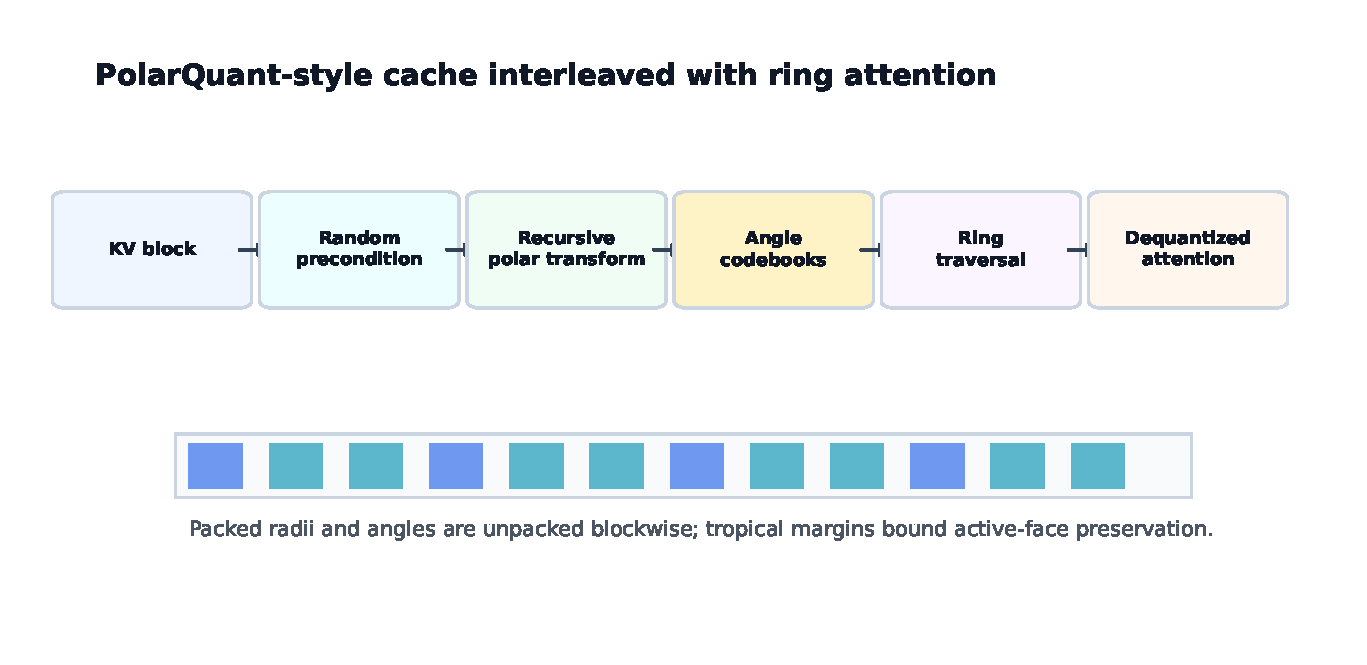
\includegraphics[width=\textwidth]{fig_polar_ring_cache.pdf}
  \caption{PolarQuant interleaving with ring attention.  Each key-value block is randomly preconditioned, recursively transformed to polar coordinates, angle-quantized, packed, and dequantized only when the block reaches a query device.}
  \label{fig:polar-ring}
\end{figure}

\begin{lemma}[Score perturbation from quantized keys]
Assume $\norm{q_i}_2\le R_Q$ for every query and $\norm{k_j-\widehat k_j}_2\le\epsilon_K$ for every key.  Then
\begin{equation}
  \norm{S-\widehat S}_\infty\le \frac{R_Q\epsilon_K}{\sqrt{d_h}}.
\end{equation}
\end{lemma}

\begin{proof}
For every pair $(i,j)$,
\begin{equation}
  \abs{S_{ij}-\widehat S_{ij}}=\frac{1}{\sqrt{d_h}}\abs{q_i\transpose(k_j-\widehat k_j)}
  \le\frac{1}{\sqrt{d_h}}\norm{q_i}_2\norm{k_j-\widehat k_j}_2
  \le\frac{R_Q\epsilon_K}{\sqrt{d_h}},
\end{equation}
by Cauchy-Schwarz.
\end{proof}

\begin{theorem}[Tropical output stability under PolarQuant cache]
Assume key and value dequantization errors obey
\begin{equation}
  \norm{k_j-\widehat k_j}_2\le\epsilon_K,
  \qquad \norm{v_j-\widehat v_j}_\infty\le\epsilon_V,
\end{equation}
and $\norm{q_i}_2\le R_Q$.  Then tropical attention with dequantized PolarQuant cache satisfies
\begin{equation}
  \norm{Y-\widehat Y}_\infty\le \frac{R_Q\epsilon_K}{\sqrt{d_h}}+\epsilon_V.
\end{equation}
If the full-precision tropical margin is larger than twice this bound, the active key is unchanged.
\end{theorem}

\begin{proof}
The previous lemma bounds score perturbation by $\epsilon_S=R_Q\epsilon_K/\sqrt{d_h}$.  Value perturbation is bounded by $\epsilon_V$.  Apply the Lipschitz and argmax-stability lemma for tropical attention.
\end{proof}

\begin{proposition}[Equivariance of a shared PolarQuant cache]
If the random preconditioner, codebooks, and quantization rules are shared over token rows and ring blocks, and block schedules are label-independent or transformed consistently, then PolarQuant-dequantized ring attention remains graph equivariant up to numerical quantization error.
\end{proposition}

\begin{proof}
The preconditioner and quantizer act identically on every key/value row.  Therefore quantizing after a row permutation gives the same packed rows in permuted order, modulo deterministic tie-breaking.  Ring traversal is a schedule; if it is label-independent or permuted with the tokens, it does not introduce semantic label dependence.  Dequantized attention is equivariant by the attention equivariance proof, with values replaced by their quantized approximations.  The only deviation from full-precision equivariance comes from finite-precision quantization and tie-breaking.
\end{proof}

\subsection{Memory accounting}

Let $B_{\mathrm{fp}}$ be bits per full-precision coordinate, typically $16$ for bf16/fp16 KV caches.  If a polar cache stores one radius using $B_r$ bits and angle level $\ell$ uses $b_\ell$ bits per angle, then amortized bits per coordinate are approximately
\begin{equation}
  B_{\mathrm{polar}}\approx \frac{B_r+\sum_{\ell=1}^{\log_2 d_h}(d_h/2^\ell)b_\ell}{d_h}+B_{\mathrm{overhead}},
\end{equation}
where $B_{\mathrm{overhead}}$ accounts for packed-index alignment and amortized codebook storage.  The compression ratio is
\begin{equation}
  \rho_{\mathrm{cache}}\approx \frac{B_{\mathrm{fp}}}{B_{\mathrm{polar}}}.
\end{equation}
Because codebooks are shared and preconditioning avoids per-block scale/zero-point storage, the overhead can be lower than blockwise affine quantization.


\section{Soft-MoE ToricGT blocks}

\subsection{Motivation and placement}

Soft-MoE is useful for ToricGT for a different reason than ordinary large-scale MoE.  The goal is not merely to increase parameter count.  The goal is to allocate typed computation to different graph-token roles without hard token dropping or brittle top-$k$ routing.  In a ToricGT block, experts may specialize as generic feed-forward maps, tropical dynamic-programming gates, toric phase maps, Hebrew root-template analyzers, local proof verifiers, or graph-decoder refiners.  Because Soft-MoE computes differentiable weighted mixtures rather than discrete assignments, the routing map remains smooth and can be made permutation equivariant.

Puigcerver, Riquelme, Mustafa, and Houlsby define Soft-MoE as a fully differentiable MoE mechanism where each expert slot receives a weighted average of all input tokens and the output tokens are reconstructed as weighted averages of the expert outputs \cite{puigcerver2024softmoe}.  ToricGT uses that mechanism as a graph-token feed-forward replacement, not as a black-box vision-only module.

\begin{figure}[t]
  \centering
  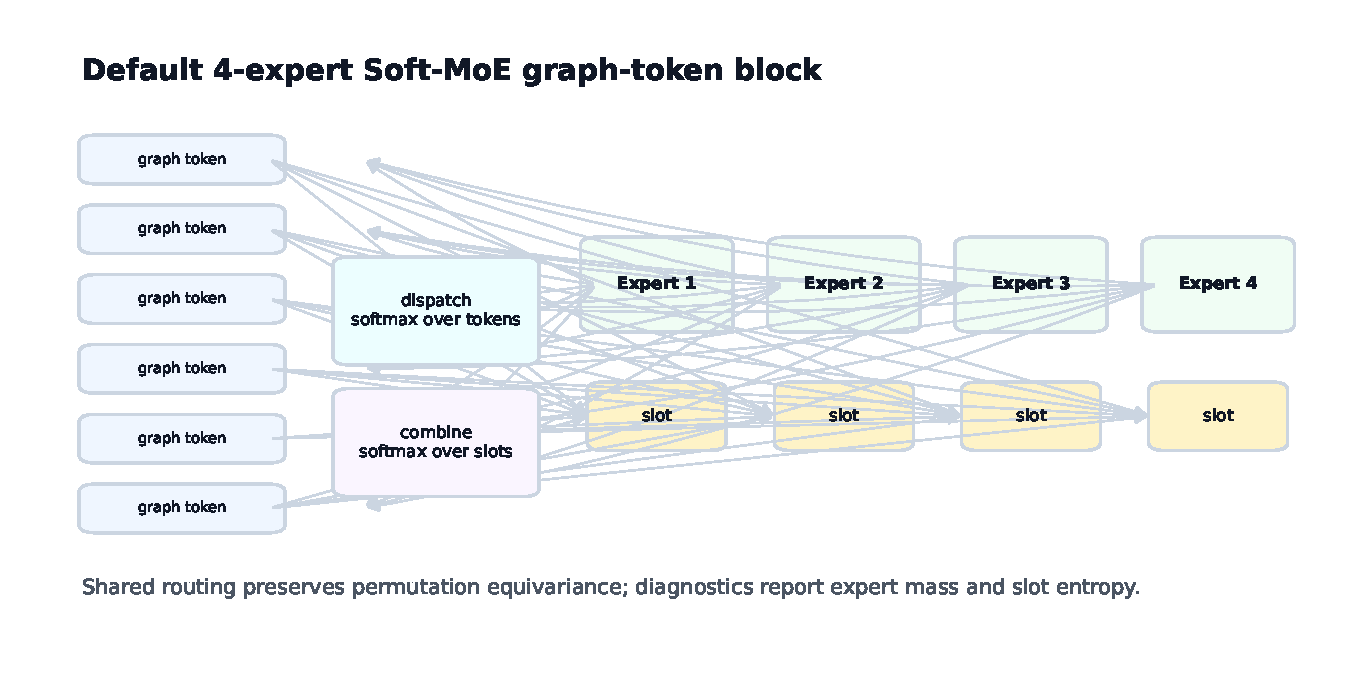
\includegraphics[width=\textwidth]{fig_soft_moe_toricgt_clean.pdf}
  \caption{Soft-MoE ToricGT block.  Graph tokens are softly dispatched into slot mixtures, typed experts process the slots, and combine weights project expert outputs back to the original token stream.  The same equations handle node, edge, proof, Hebrew, tropical, and toric tokens when masks and type channels are equivariant.}
  \label{fig:soft-moe-toricgt}
\end{figure}

\subsection{Equations}

Let $X\in\R^{B\times L\times d}$ be a batch of graph-token hidden states and let $M\in\{0,1\}^{B\times L}$ be the validity mask.  A Soft-MoE layer has $E$ experts and $S$ slots per expert.  Let $\Phi\in\R^{d\times E\times S}$ be learned slot vectors and let $g>0$ be a learned temperature.  Use normalized vectors
\begin{equation}
  \bar x_{b i}=\frac{x_{b i}}{\norm{x_{b i}}_2+\epsilon},\qquad
  \bar\phi_{e s}=\frac{\phi_{e s}}{\norm{\phi_{e s}}_2+\epsilon},
\end{equation}
and define token-slot logits
\begin{equation}
  A_{b i e s}=g\,\ip{\bar x_{b i}}{\bar\phi_{e s}}.
\end{equation}
Invalid tokens are removed by setting $A_{b i e s}=-\infty$ whenever $M_{b i}=0$.  Dispatch weights normalize over tokens for each slot:
\begin{equation}
  D_{b i e s}=\frac{\exp(A_{b i e s})M_{b i}}{\sum_{j=1}^L\exp(A_{b j e s})M_{b j}+\epsilon}.
\end{equation}
Combine weights normalize over slots for each token:
\begin{equation}
  C_{b i e s}=\frac{\exp(A_{b i e s})}{\sum_{e'=1}^E\sum_{s'=1}^S\exp(A_{b i e's'})+\epsilon}.
\end{equation}
The input slot for expert $e$ and slot $s$ is
\begin{equation}
  Z_{b e s}=\sum_{i=1}^L D_{b i e s}X_{b i}.
\end{equation}
Each expert $f_e:\R^d\to\R^d$ processes its slots:
\begin{equation}
  \widetilde Z_{b e s}=f_e(Z_{b e s}).
\end{equation}
The output token is reconstructed by
\begin{equation}
  Y_{b i}=\sum_{e=1}^E\sum_{s=1}^S C_{b i e s}\widetilde Z_{b e s}.
\end{equation}
A residual gate $\alpha_\ell\in[0,1]$ is used in practice:
\begin{equation}
  X_{\ell+1}=X_\ell+\alpha_\ell\operatorname{Dropout}(Y_\ell),\qquad \alpha_\ell\text{ initialized near }0.05\text{ or }0.1.
\end{equation}
This conservative initialization prevents the expert bank from dominating early training before the graph-token features have useful semantics.

\begin{lemma}[Soft-MoE graph-token equivariance]
Let $P$ be a token permutation matrix that preserves the validity mask by $M(PX)=PM(X)$.  Suppose $\Phi$, the experts $f_e$, and the temperature $g$ are shared across token rows and do not depend on absolute token indices.  Then
\begin{equation}
  \operatorname{SoftMoE}(PX,PM)=P\operatorname{SoftMoE}(X,M).
\end{equation}
\end{lemma}

\begin{proof}
The logits satisfy
\begin{equation}
  A(PX)_{i e s}=A(X)_{\pi^{-1}i,e,s}.
\end{equation}
The dispatch denominator for a fixed $(e,s)$ sums over all valid tokens, so it is invariant under reindexing.  Therefore
\begin{equation}
  D(PX)_{i e s}=D(X)_{\pi^{-1}i,e,s}.
\end{equation}
The slot mixture is unchanged:
\begin{align}
  Z(PX)_{e s}
    &=\sum_i D(PX)_{i e s}(PX)_i
      =\sum_i D(X)_{\pi^{-1}i,e,s}X_{\pi^{-1}i}\nonumber\\
    &=\sum_j D(X)_{j e s}X_j
      =Z(X)_{e s}.
\end{align}
Thus expert outputs $\widetilde Z_{e s}$ are unchanged.  The combine weights satisfy $C(PX)_{i e s}=C(X)_{\pi^{-1}i,e,s}$ because their denominator normalizes only over slots for the same token.  Hence
\begin{equation}
  Y(PX)_i=\sum_{e,s}C(X)_{\pi^{-1}i,e,s}\widetilde Z_{e s}=Y(X)_{\pi^{-1}i},
\end{equation}
which is exactly $PY(X)$.
\end{proof}

\begin{proposition}[Soft-MoE preserves TokenGT equivariance]
Replacing any shared token-wise feed-forward block of an equivariant ToricGT layer by the Soft-MoE block above preserves graph-to-graph equivariance.
\end{proposition}

\begin{proof}
The surrounding attention, normalization, residual, and decoder maps are equivariant by earlier results.  The Soft-MoE block is equivariant by the preceding lemma.  Compositions and residual sums of equivariant maps are equivariant.
\end{proof}

\subsection{Typed expert bank for ToricGT}

For the full 8M-35M graph-reasoning model, use a small typed bank rather than hundreds of experts.
\begin{longtable}{p{0.22\linewidth}p{0.31\linewidth}p{0.36\linewidth}}
\toprule
Expert & Function & Practical notes \\
\midrule
\endhead
Generic MLP & ordinary dense nonlinear map & always present; fallback for arbitrary continuous approximation \\
Tropical DP & max/min-plus candidate scoring and margin features & use for shortest path, Viterbi, active-face, and transitive-closure tasks \\
Toric phase & clock/shift/cocycle channels and phase normalization & regularize lightly; avoid forcing phase structure on arbitrary data \\
Hebrew root & radical alignment, template/binyan features, paradigm consistency & useful only for Hebrew or Semitic morphology batches; can be gated by type embeddings \\
Proof verifier & local step validity and dependency consistency & attach to equation/proof-obligation nodes \\
Graph decoder & node/edge graph-to-graph refinement & useful near output layers \\
\bottomrule
\end{longtable}

Recommended defaults are $E=4$--$8$ experts, $S=1$--$4$ slots per expert, $g$ initialized near $1$, and Soft-MoE enabled by default in the upper half of the network.  For $L\le2048$, $E S\le32$ is normally safe on a 4090.  For longer graph traces, use chunked dispatch: compute $A$ blockwise over tokens, accumulate dispatch denominators by log-sum-exp, then form slots in a second streaming pass.  This keeps the slot computation compatible with ring attention.

\subsection{Implementation details}

A minimal PyTorch implementation for graph tokens has the following shape discipline.
\begin{verbatim}
# X: [B, L, d], mask: [B, L]
Xn = l2_normalize(X, dim=-1)
Pn = l2_normalize(Phi, dim=0)                 # [d, E, S]
logits = scale * torch.einsum('bld,des->bles', Xn, Pn)
logits = logits.masked_fill(~mask[:, :, None, None], -torch.inf)
D = torch.softmax(logits, dim=1)              # dispatch over tokens
C = torch.softmax(logits.flatten(2), dim=-1).view(B, L, E, S)
slots = torch.einsum('bld,bles->besd', X, D)
out_slots = stack([experts[e](slots[:, e]) for e in range(E)], dim=1)
Y = torch.einsum('besd,bles->bld', out_slots, C)
X = X + residual_gate * dropout(Y)
\end{verbatim}
The implementation should explicitly test: output shape, mask handling, gradient finiteness, deterministic behavior under token permutation, absence of NaNs when all tokens of a batch element are padded, and agreement between chunked and unchunked dispatch within numerical tolerance.


\subsection{Prefix-causal Soft-MoE for language-model scoring}

The graph-to-graph ToricGT encoder is allowed to use bidirectional graph context.  The Parameter-Golf micro language model is not.  A direct Soft-MoE implementation that dispatches each expert slot using all tokens in a sequence is noncausal: the slot representation for position $t$ would include future tokens $x_{>t}$ and would therefore leak validation information.  The contest-facing model must use a prefix-causal version of Soft-MoE whenever the output at token $t$ is scored autoregressively.

Flatten the expert and slot indices into $s\in\{1,\dots,E S\}$ and let $a_{t s}$ be the token-slot logit.  For an autoregressive sequence $x_1,\dots,x_T$, define strict-prefix dispatch accumulators
\begin{align}
  N_s^{(t)} &= \sum_{m<t}\exp(a_{m s})x_m,\\
  R_s^{(t)} &= \sum_{m<t}\exp(a_{m s}),\\
  Z_s^{(t)} &= \frac{N_s^{(t)}}{R_s^{(t)}+\epsilon}.
\end{align}
The expert output available at position $t$ is
\begin{equation}
  \widetilde Z_s^{(t)}=f_{e(s)}\!\left(Z_s^{(t)}\right),
\end{equation}
and the causal combine weights are normalized only over slots for the current token,
\begin{equation}
  C_{t s}=\frac{\exp(a_{t s})}{\sum_{u=1}^{E S}\exp(a_{t u})+\epsilon}.
\end{equation}
The Soft-MoE residual used to predict token $x_{t+1}$ is then
\begin{equation}
  y_t=\sum_{s=1}^{E S}C_{t s}\widetilde Z_s^{(t)}.
\end{equation}
After the loss for position $t$ has been computed, the accumulators may be updated by
\begin{align}
  N_s^{(t+1)} &= N_s^{(t)}+\exp(a_{t s})x_t,\\
  R_s^{(t+1)} &= R_s^{(t)}+\exp(a_{t s}).
\end{align}
This is a score-before-update rule.  It is the Soft-MoE analogue of ordinary causal attention: the current prediction can use only the strict prefix.

\begin{lemma}[Prefix-causal Soft-MoE is valid for autoregressive BPB]
For every position $t$, the output $y_t$ of the prefix-causal Soft-MoE block is a measurable function of $x_{<t}$, the current unscored embedding used to choose a distribution over $x_t$ only when that embedding itself is derived from $x_{<t}$, and the fixed model parameters.  In particular, if the surrounding attention and embedding pipeline is causal, replacing a dense feed-forward block by prefix-causal Soft-MoE preserves strict left-to-right scoring.
\end{lemma}

\begin{proof}
By construction, $N_s^{(t)}$ and $R_s^{(t)}$ are sums over indices $m<t$.  Therefore $Z_s^{(t)}$ and $\widetilde Z_s^{(t)}$ are functions only of the strict prefix and the parameters of $f_e$.  The combine weights $C_{t s}$ may depend on the hidden state at $t$, but in a causal language model that hidden state is produced from the same strict prefix.  Hence $y_t$ is a function of the strict prefix.  The update with $x_t$ occurs only after scoring position $t$, so no scored probability can depend on its own target or on future targets.
\end{proof}

A vectorized training implementation can compute these quantities by prefix scans.  In PyTorch, the noncausal dispatch
\begin{verbatim}
D = softmax(logits, dim=1)          # invalid for LM scoring if dim=1 sees future
slots = einsum('bld,bles->besd', X, D)
\end{verbatim}
should be replaced in the contest model by cumulative sums over time:
\begin{verbatim}
w = torch.exp(logits.flatten(2)).clamp_max(1e4)       # [B, T, ES]
prefix_num = torch.cumsum(w[..., None] * X[:, :, None, :], dim=1)
prefix_den = torch.cumsum(w, dim=1)
# strict prefix: shift right before forming slots
N = torch.cat([zeros_like(prefix_num[:, :1]), prefix_num[:, :-1]], dim=1)
R = torch.cat([zeros_like(prefix_den[:, :1]), prefix_den[:, :-1]], dim=1)
slots_t = N / (R[..., None] + eps)                    # [B, T, ES, d]
out_slots_t = experts(slots_t)
C = torch.softmax(logits.flatten(2), dim=-1)
Y = torch.einsum('bts,btsd->btd', C, out_slots_t)
\end{verbatim}
For the graph-reasoning encoder this causal restriction is unnecessary; for the Parameter-Golf track it is mandatory.

\subsection{Soft-MoE regularizers and diagnostics}

Soft-MoE should be monitored rather than trusted.  Define expert combine mass
\begin{equation}
  m_e=\frac{1}{B L}\sum_{b,i,s}C_{b i e s},
\end{equation}
slot dispatch entropy
\begin{equation}
  H_{e s}^{D}=-\sum_i D_{b i e s}\log(D_{b i e s}+\epsilon),
\end{equation}
and token combine entropy
\begin{equation}
  H_i^C=-\sum_{e,s}C_{b i e s}\log(C_{b i e s}+\epsilon).
\end{equation}
A light usage regularizer is
\begin{equation}
  \mathcal L_{\mathrm{moe}}=\lambda_{\mathrm{bal}}\sum_e\left(m_e-\frac1E\right)^2
  -\lambda_D\Eop[H^D]+\lambda_C\Eop\left[\max(0,H^C-H_{\max})\right].
\end{equation}
The sign convention encourages noncollapsed dispatch while allowing combine weights to become sharp only when the task supports specialization.  Do not over-regularize $m_e$ on mixed-domain batches: if a batch contains only Hebrew morphology, the Hebrew-root expert should be allowed to receive more mass.

\section{Parameter-Golf constrained ToricGT}

\subsection{Contest constraints as engineering axioms}

The OpenAI Model Craft Challenge: Parameter Golf asks participants to train the best language model that fits in a self-contained $16{,}000{,}000$ byte artifact, trains in roughly ten minutes on the prescribed 8xH100 evaluation setting, and is scored by tokenizer-agnostic bits per byte on FineWeb validation data \cite{openai2026paramgolf}.  The important engineering point is that the counted artifact is not a vague parameter count: it is the serialized code, compressed model state, tokenizer or byte model, and metadata that the evaluator receives.  The contest setting also requires evaluation to be self-contained, with no network calls, no external downloads, no hidden validation side information, and no dependence on a training dataset at evaluation time \cite{openai2026paramgolf}.  Record-style submissions should include a runnable \texttt{train\_gpt.py}, README, \texttt{submission.json}, training logs from independent runs, and exact byte accounting.  SOTA claims require a statistically meaningful improvement over the current record, so a ToricGT-derived submission must be treated as an auditable compression experiment rather than an informal model sketch.

\begin{figure}[t]
  \centering
  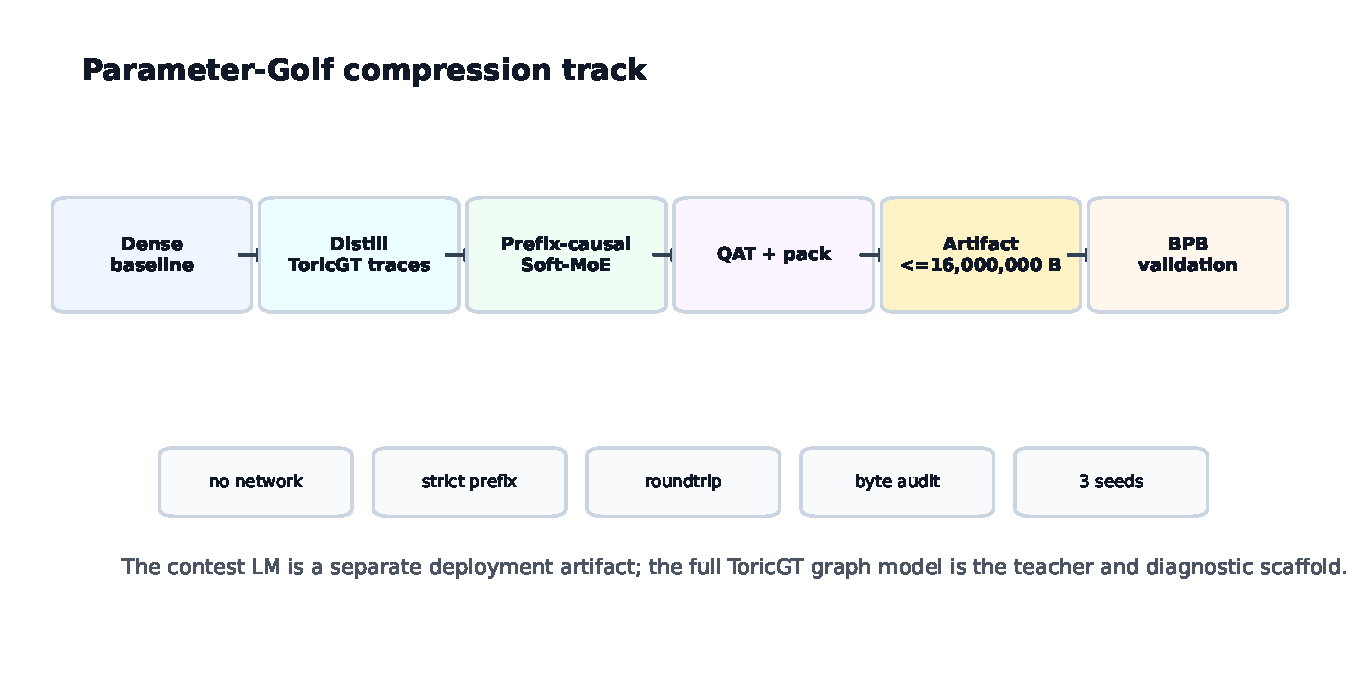
\includegraphics[width=\textwidth]{fig_parameter_golf_protocol_clean.pdf}
  \caption{Parameter-Golf protocol for ToricGT.  The full graph-to-graph model remains the research model.  The contest-facing model is a micro language model distilled from graph-reasoning traces, equipped with byte-safe Soft-MoE adapters, trained under the wallclock budget, and exported as a single self-contained artifact with exact byte accounting and prequential BPB validation.}
  \label{fig:param-golf-pipeline}
\end{figure}

\begin{definition}[Parameter-Golf artifact budget]
Let
\begin{equation}
  B_{\mathrm{art}}=B_{\mathrm{code}}+B_{\mathrm{weights}}+B_{\mathrm{tokenizer}}+B_{\mathrm{metadata}}.
\end{equation}
A Parameter-Golf-compliant artifact must satisfy
\begin{equation}
  B_{\mathrm{art}}\le16{,}000{,}000.
\end{equation}
For a model with tensors $W_r$ quantized to $b_r$ bits per scalar and entropy-compressed by factor $\rho_r\ge1$,
\begin{equation}
  B_{\mathrm{weights}}\approx\sum_r \frac{b_r\,|W_r|}{8\rho_r}+B_{\mathrm{packing}}.
\end{equation}
\end{definition}

The contest objective can be written as
\begin{equation}
  \min_{\theta,\mathcal C}\operatorname{BPB}_{\mathrm{FineWeb}}(q_{\theta,\mathcal C})
  \quad\text{subject to}\quad
  B_{\mathrm{art}}\le16{,}000{,}000,
\end{equation}
where $\mathcal C$ denotes the compression/export scheme and
\begin{equation}
  \operatorname{BPB}(q)= -\frac{1}{N_{\mathrm{bytes}}}\sum_{t}\log_2 q(b_t\mid b_{<t}).
\end{equation}
This formula is tokenizer-agnostic because the denominator is bytes, not tokens.

\subsection{Prequential BPB validity}

Parameter Golf scoring is best viewed as a prequential compression game.  The model emits a full normalized predictive distribution, pays log loss on the next symbol, and only then may update any legal online state.  Let the validation byte stream be $b_1,\dots,b_T$ and let $\ell(t)$ be the exact number of bytes represented by the tokenizer symbol scored at step $t$.  A scoring procedure is valid if it satisfies four conditions:
\begin{enumerate}[leftmargin=2em]
  \item \textbf{strict prefix dependence}: $q_t$ depends only on $b_{<t}$, fixed parameters, and legal online state derived from already scored bytes;
  \item \textbf{full normalization}: $q_t$ is a normalized distribution over the next scored symbol;
  \item \textbf{score before update}: the state update using $b_t$ occurs after $-\log q_t(b_t)$ is recorded;
  \item \textbf{single validation pass}: the validation stream is not permuted, repeated for tuning, or searched over by seeds.
\end{enumerate}
Under these conditions the reported objective is
\begin{equation}
  \operatorname{BPB}_{\mathrm{valid}}
  =\frac{\sum_{t=1}^{T}-\log_2 q_t(b_t\mid b_{<t})}{\sum_{t=1}^{T}\ell(t)}.
\end{equation}

\paragraph{Metric taxonomy and SP1024 conversion.}
The implementation keeps three FineWeb quantities separate.  The official
Parameter-Golf quantity is the byte-denominated score above; it is logged only
when a byte-level or score-before-update evaluator has actually produced it.
The TokenGT research model also exposes a graph-node SP1024 language-model
head.  For a graph batch with SP1024 targets $z_1,\ldots,z_m$ and graph-node
predictive distributions $p_i$, its native scalar is
\begin{equation}
  \operatorname{BPT}_{\mathrm{SP1024}}
  =
  \frac{1}{m}\sum_{i=1}^{m}-\log_2 p_i(z_i),
\end{equation}
bits per SP1024 graph node.  This number is useful for checking whether the
graph LM head is learning, but it is not the Parameter-Golf BPB because its
denominator is graph-token count, not UTF-8 bytes.  When the SP1024 shard and
tokenizer are available, ToricGT also reports a sample-aligned byte-normalized
proxy.  Let $D(z_{1:m})$ be the UTF-8 string obtained by decoding the scored
target SP1024 sequence and set
\begin{equation}
  \widehat\rho_{\mathrm{bytes/token}}
  =
  \frac{\operatorname{bytes}(D(z_{1:m}))}{m}.
\end{equation}
Then the reported proxy is
\begin{equation}
  \widehat{\operatorname{BPB}}_{\mathrm{SP1024}\to\mathrm{byte}}
  =
  \frac{\operatorname{BPT}_{\mathrm{SP1024}}}
       {\widehat\rho_{\mathrm{bytes/token}}}
  =
  \frac{\sum_i-\log_2 p_i(z_i)}
       {\operatorname{bytes}(D(z_{1:m}))}.
\end{equation}
This conversion is valid as a diagnostic normalization for a bidirectional or
otherwise non-score-valid graph-node head, and it is often more interpretable
than raw SP1024 bits/token.  It is still marked as estimated unless the
TokenGT path is made genuinely autoregressive.  The native causal TokenGT
route does this by attaching a learned SP1024 input-token embedding to each
node, carrying a reveal-rank tensor through the graph batch, and replacing
bidirectional graph attention by the mask
\begin{equation}
  M_{ij}=1\quad\Longleftrightarrow\quad
  i,j\text{ are valid tokens and } r(j)\le r(i).
\end{equation}
FineWeb chains use $r(i)=i$, directed acyclic reasoning graphs use a
topological rank, and cyclic or noncausal graphs use a deterministic
content-independent random reveal rank.  Edge-token rank is the maximum of
its endpoint ranks.  Under these hypotheses the SP1024 graph-node loss is a
score-before-update next-token loss, and the byte denominator is the sum of
SentencePiece target byte increments, so the restricted FineWeb metric can be
reported as an OAI-style BPB for this route.  Without these hypotheses it
remains a proxy.  Thus dashboards must display all relevant concepts under
different names:
\[
\operatorname{BPB}_{\mathrm{OAI,official}},\qquad
\operatorname{BPT}_{\mathrm{SP1024,TokenGT}},\qquad
\operatorname{BPB}_{\mathrm{SP1024,causal\ TokenGT}},\qquad
\widehat{\operatorname{BPB}}_{\mathrm{SP1024}\to\mathrm{byte}}.
\]
Only score-valid byte or causal-token metrics should decide Parameter-Golf
success; bidirectional graph proxies guide TokenGT representation training
and ablations.

\paragraph{OAI baseline transfers to causal TokenGT.}
The causal TokenGT route ports the competition baseline's efficient input
conditioning rather than replacing TokenGT by the baseline.  The transferred
features are all measurable before the current symbol is scored:
\begin{enumerate}[leftmargin=2em]
  \item \emph{Tied SP1024 output head}: the graph-node LM logits are computed
  with the learned SP1024 input embedding matrix, saving one dense output
  projection and aligning input/output geometry.
  \item \emph{Recurrent block passes}: the same stored TokenGT blocks may be
  applied multiple times, increasing computation per artifact byte as in the
  dense Parameter-Golf adapter.
  \item \emph{Target-position and toric phase features}: public target
  positions contribute a learned position embedding and a four-dimensional
  toric phase vector
  $(\sin 2\pi\theta p,\cos 2\pi\theta p,\sin 2\pi\sqrt2\,p,\cos 2\pi\sqrt2\,p)$.
  \item \emph{Strict-prefix hash context}: the previous revealed input token,
  the current already-revealed input token, the public target position, and
  the reveal rank are hashed into a small embedding table.  This is the
  TokenGT analogue of the OAI baseline's cheap n-gram memory.
  \item \emph{Revealed-neighbor hash}: for each graph edge with endpoints
  $u,v$, the node $u$ may contribute a compact hash embedding to $v$ only when
  $\rho(u)<\rho(v)$, where $\rho$ is the FineWeb linear rank, the DAG
  topological rank, or the deterministic random reveal rank.  Thus the module
  is graph-structured while remaining score-before-update measurable:
  \[
    h_v^{\mathrm{nbr}}
    =
    \frac{1}{\max(1,|\mathcal N^-_\rho(v)|)}
    \sum_{u\in\mathcal N(v):\,\rho(u)<\rho(v)}
    E_{\mathrm{nbr}}\!\left(
      \operatorname{hash}(x_u,x_v,p_v,\rho(v),\operatorname{dir}(u,v))
    \right).
  \]
  \item \emph{SP CaseOps}: instead of byte classes, the graph route computes
  SentencePiece operator features from the already revealed input id: control,
  unknown, byte-token, leading-space, alphabetic, digit, punctuation, non-ASCII,
  and normalized id indicators.
  \item \emph{SmearGate}: a small input-dependent temperature rescales logits
  after the graph hidden state is computed.
\end{enumerate}
The dense $1024\times1024$ bigram table remains an ablation, but the default
route uses smaller prefix and revealed-neighbor hash tables to preserve
artifact margin under the $16{,}000{,}000$ byte cap.  None of these transferred
modules may inspect the unscored target SP token; on noncausal or cyclic
graphs, their ordering signal is the deterministic random reveal rank rather
than an artificial direction.

\paragraph{Byte-scored TokenGT hybrid objective.}
The clean way to use TokenGT structure in the contest-facing branch is not to
replace byte scoring by graph-token scoring.  Instead, ToricGT keeps a
byte-level random-order language model and attaches a TokenGT-style graph loss
to its hidden reveal trajectory.  Let $\pi$ be the random reveal permutation,
let $h_k$ be the hidden state used to score $b_{\pi_k}$, and let
$p_k=\pi_k$ be the original byte position.  The internal graph has vertices
$v_k=(h_k,p_k)$ and local path-neighborhood edges
\begin{equation}
  A_{ij}=\mathbf 1\{0<|p_i-p_j|\le r\}.
\end{equation}
When the source admits a meaningful causal orientation, the directed edge label
is $E_{ij}=A_{ij}\mathbf 1\{i<j\}$, so edges point from earlier scored vertices
to later scored vertices.  This is the ordinary FineWeb path graph made
score-before-update compatible.  When a source graph is undirected, cyclic, or
has no trusted causal semantics, ToricGT sets $E_{ij}=A_{ij}$ and disables the
direction and cycle penalties below; the graph loss then acts only as an
undirected structural regularizer.

With $s_{ij}=\langle \bar h_i,\bar h_j\rangle/\tau$, coarse byte-class label
$C_{ij}$, hidden distance $d_h(i,j)$, and toric phase map $\phi(p)$, the
implemented differentiable objective is
\begin{align}
  \mathcal L_{\mathrm{ByteTokenGT}}
  &=
  a_e\,\mathrm{BCE}(s_{ij},E_{ij})
  +a_p\,\mathrm{SmoothL1}\!\left(d_h(i,j),\frac{\log(1+|p_i-p_j|)}{\log(1+\max |p_a-p_b|)}\right)\\
  &\quad
  +a_c\,\mathrm{BCE}(s_{ij},C_{ij})
  +a_d\,\mathbb E_{i\to j}\left[\max\{0,m-\cos(h_j-h_i,\phi(p_j)-\phi(p_i))\}^2\right]\\
  &\quad
  +a_{\mathrm{cyc}}\,
  \mathbb E_{\substack{A_{ij}=1\\ i>j}}\sigma(s_{ij}).
\end{align}
The $a_d$ and $a_{\mathrm{cyc}}$ terms are multiplied by zero under the
noncausal policy.  The full loss used by the hybrid run is then
\begin{equation}
  \mathcal L
  =
  \mathcal L_{\mathrm{byte\ CE}}
  +\lambda_{\mathrm{ByteTokenGT}}\mathcal L_{\mathrm{ByteTokenGT}}
  +\lambda_{\mathrm{GFN}}\mathcal L_{\mathrm{TB}}
  +\lambda_{\mathrm{GraphCG}}\mathcal L_{\mathrm{GraphCG}}
  +\lambda_{\mathrm{TBGG}}\mathcal L_{\mathrm{TBGG}}
  +\lambda_{\mathrm{Koszul}}\mathcal L_{\mathrm{Koszul}}
  +\lambda_{\mathrm{Slepian}}\mathcal L_{\mathrm{Slepian}}
  +\lambda_{\mathrm{mem}}\mathcal L_{\mathrm{memory}}
  +\cdots.
\end{equation}
Thus the advanced graph, toric, topological, BGG, Koszul, Slepian--Pollak,
GFlowNet, GraphCG, and memory terms are bona fide optimizer objectives with
explicit weights.  The byte CE term remains primary because it is exactly the
quantity whose average in base two gives official BPB.  The auxiliary weights
are intentionally small at step zero and can be raised by phase curricula after
the restricted FineWeb BPB slope is stable.
In the current byte-accounted configuration the hybrid branch uses
$d=448$, $8$ heads, seven stored dense blocks, and two recurrent passes.  A
6-bit row-quantized LZMA artifact probe is $15{,}206{,}131$ bytes, leaving
$793{,}869$ bytes under the $16{,}000{,}000$ byte model-artifact cap; if a
future counted bundle includes more code, the $d=416$ variant is the safer
fallback.

\begin{proposition}[Score-before-update prevents validation leakage]
Assume $q_t$ satisfies strict prefix dependence and the online state update has the form $s_{t+1}=U(s_t,b_t)$ after the loss term at $t$ is recorded.  Then the cumulative validation loss is a proper left-to-right log score and no term in the sum can depend on future validation bytes.
\end{proposition}

\begin{proof}
We prove by induction that $s_t$ is a function only of $b_{<t}$ and fixed parameters.  The base state $s_1$ is fixed.  If $s_t$ is a function only of $b_{<t}$, then $q_t$ is also a function only of $b_{<t}$ by strict prefix dependence.  The loss term $-\log q_t(b_t)$ is therefore scored before any access to $b_{>t}$.  The update $s_{t+1}=U(s_t,b_t)$ is then a function only of $b_{\le t}$, closing the induction.  Thus no loss term uses future information.
\end{proof}

\subsection{Random-order graph autoregressive projection}

The contest-facing implementation uses a graph-to-sequence projection rather than replacing the ToricGT theory.  A byte chunk $b=(b_1,\ldots,b_T)$ is viewed as a path graph whose nodes are byte positions.  For every chunk, sample a content-independent permutation
\begin{equation}
  \pi=\pi(s,\mathrm{id},r,T)\in S_T
\end{equation}
from a base seed $s$, a public sample id, a pass id $r$, and the length $T$.  The randomized autoregressive factorization is
\begin{equation}
  q_\theta(b\mid \pi)=\prod_{k=1}^T q_\theta\left(b_{\pi_k}\mid b_{\pi_1},\ldots,b_{\pi_{k-1}},\pi_1,\ldots,\pi_k\right).
\end{equation}
The row scored at step $k$ contains the previous revealed byte, the current target position $\pi_k$, fixed toric phase features of $\pi_k$, and causal access only to rows $<k$.  It does not contain $b_{\pi_k}$.

The same rule is used when TokenGT receives graph inputs rather than byte rows.
If the graph already has a trusted causal orientation and is acyclic, the reveal
rank is a topological order.  If the graph is a FineWeb token chain, the reveal
rank is the usual left-to-right order.  If the graph is cyclic, undirected, or
otherwise noncausal, ToricGT samples a deterministic random reveal order from
the record id and node ids.  This is the graph-token analogue of random-order
autoregressive decoding: it avoids future-node leakage without pretending that
an undirected cycle has a natural causal direction.

\begin{lemma}[Content-independent random order is score-valid]
If $\pi$ is sampled independently of the unscored byte values and the model row for step $k$ is a measurable function only of $(b_{\pi_1},\ldots,b_{\pi_{k-1}},\pi_1,\ldots,\pi_k)$ and fixed parameters, then every loss term
\begin{equation}
  -\log q_\theta(b_{\pi_k}\mid b_{\pi_{<k}},\pi_{\le k})
\end{equation}
is score-before-update valid.
\end{lemma}

\begin{proof}
Induct on $k$.  Before step $1$, only the permutation, BOS symbol, and fixed parameters are known.  Assume before step $k$ that the online state is a function only of already scored bytes $b_{\pi_{<k}}$ and the public order prefix $\pi_{\le k}$.  The predictive distribution for $b_{\pi_k}$ is computed from exactly those quantities.  The byte $b_{\pi_k}$ is inserted into the state only after its log score is recorded.  Since $\pi$ is independent of unscored byte values, the order itself cannot encode future validation information.
\end{proof}

\subsection{Byte-safe embedding-space GFlowNet actions}

The full ToricGT graph model uses an embedding-space GFlowNet over graph-of-thought states.  The Parameter-Golf adapter uses the score-valid subset of the same idea.  Let $h_k$ be the hidden state at random-order step $k$, computed from $(b_{\pi_{<k}},\pi_{\le k})$.  A small policy head produces
\begin{equation}
  p_\psi(a\mid h_k)=\softmax(W_2\sigma(W_1\operatorname{LN}(h_k)))_a,
  \qquad a\in\{1,\ldots,A\}.
\end{equation}
Each action has an embedding $u_a\in\R^d$, and the byte predictor uses
\begin{equation}
  \widetilde h_k=h_k+\alpha u_{a_k},\qquad
  q_\theta(b_{\pi_k}\mid b_{\pi_{<k}},\pi_{\le k},a_k)=\softmax(E\widetilde h_k+c).
\end{equation}
At evaluation, multiple action trajectories may be averaged by the legal mixture
\begin{equation}
  q_\theta^{(M)}(b_{\pi_k}\mid\mathcal F_k)
  =\frac1M\sum_{m=1}^M q_\theta(b_{\pi_k}\mid \mathcal F_k,a_k^{(m)}),
  \qquad a_k^{(m)}\sim p_\psi(\cdot\mid h_k),
\end{equation}
where $\mathcal F_k$ is the prefix sigma-field generated by already scored bytes and public order information.  A lightweight trajectory-balance surrogate uses the detached next-byte log likelihood as a local reward proxy:
\begin{equation}
  \mathcal L_{\mathrm{PG\text{-}GFN}}
  =
  \Eop_k\left(\log Z_\psi+\log p_\psi(a_k\mid h_k)+
  \operatorname{CE}_k^\mathrm{stop}\right)^2
  -\lambda_H\Eop_k H(p_\psi(\cdot\mid h_k)).
\end{equation}
This is not a substitute for the full graph GFlowNet objective; it is a compact, byte-accounted way to let the contest model explore latent graph-of-thought refinements at training and inference time.

\begin{lemma}[GFlowNet action scaling is score-valid]
If $h_k$ is $\mathcal F_k$-measurable and $a_k$ is sampled from $p_\psi(\cdot\mid h_k)$ before observing $b_{\pi_k}$, then scoring with $q_\theta(\cdot\mid\mathcal F_k,a_k)$ and updating state after the score preserves prequential validity.
\end{lemma}

\begin{proof}
The sampled action is a randomized function of $h_k$ and independent sampler noise.  Since $h_k$ is $\mathcal F_k$-measurable, the pair $(h_k,a_k)$ is measurable with respect to $\mathcal F_k$ augmented by legal internal randomness.  The distribution $q_\theta(\cdot\mid\mathcal F_k,a_k)$ is therefore fixed before $b_{\pi_k}$ is read.  The update including $b_{\pi_k}$ occurs after recording the log score, so the score-before-update induction remains unchanged.
\end{proof}

\subsection{Relative Kolmogorov diagnostics and analogical helper transfer}

The competition objective is BPB, but BPB alone does not reveal whether a small model has learned reusable reasoning programs.  ToricGT therefore reports compressor-tagged conditional-complexity proxies.  For a compressor $c$, define
\begin{equation}
  \widehat K_c(s)=|c(s)|,\qquad
  \widehat K_c(y\mid x)=\max\{0,\widehat K_c(x\Vert y)-\widehat K_c(x)\}.
\end{equation}
This is not true Kolmogorov complexity, which is uncomputable; it is an auditable estimator whose compressor and helper context are always named.  The underlying ideal quantities are the conditional complexities
\begin{equation}
  K_U(y\mid x)=\min\{|p|:U(p,x)=y\},\qquad
  K_U(x\mid y)=\min\{|p|:U(p,y)=x\},
\end{equation}
for a fixed universal machine $U$.  Up to the invariance constant, these measure how much extra program information is needed to reconstruct one object from the other.  The two directions matter.  In ToricGT, $x$ is usually a problem, graph prefix, or helper trajectory, while $y$ is a target answer, future byte block, or reasoning trace; $K(y\mid x)$ measures forward reasoning economy, whereas $K(x\mid y)$ measures how much of the original problem structure is recoverable from the proposed solution.  A short answer with low $K(y\mid x)$ but high $K(x\mid y)$ can be an overcompressed guess rather than a faithful solution.

For diagnostics that allow signed improvement over the best direct helper, ToricGT also logs
\begin{equation}
  \widetilde K_c(y\mid x;h_0)=\widehat K_c(h_0\Vert y)-\widehat K_c(h_0)-\widehat K_c(y\mid x),
\end{equation}
where $h_0$ is a named baseline helper such as the strict prefix or shortest-known direct program proxy.  Negative values mean that the new helper encoded $y$ more compactly than the baseline proxy.  These signed values are never interpreted as negative true Kolmogorov complexity; they are relative compression gains.

For random-order autoregression, the helper object is structured.  At random-order step $k$, the direct helper family is
\begin{equation}
  H_k=\{b_{\pi_{<k}},\pi,\operatorname{chunk}(b),a_{<k},G_k,T_k\},
\end{equation}
where $b_{\pi_{<k}}$ is the strict prefix, $\pi$ is the public permutation or tree-order program, $\operatorname{chunk}(b)$ is the original graph-projected byte chunk, $a_{<k}$ is the prefix-visible GFlowNet action trace when active, and $G_k,T_k$ are optional serialized graph and tree helper payloads.  The reported shortest-known program proxy is
\begin{equation}
  \widehat K_c(y_k\mid H_k)
  =\min_{h\in H_k\cup\{\varnothing\}}\widehat K_c(y_k\mid h).
\end{equation}
This construction interacts correctly with random-order decoding: the public order program and strict prefix are available before scoring, while the target byte is not.

Analogical reasoning supplies additional helper objects.  Given a source pair $(x_s,y_s)$ and target pair $(x_t,y_t)$, plus optional source graph/tree serializations $(G_s,T_s)$, define the transfer residual
\begin{equation}
  \Delta K_c^{\mathrm{ana}}
  =
  \widehat K_c(y_t\mid H_t,x_s,y_s,G_s,T_s)
  -
  \widehat K_c(y_t\mid H_t).
\end{equation}
Negative $\Delta K_c^{\mathrm{ana}}$ means the analogy shortened the estimated program for the target.  The implementation logs both this signed residual and the clipped gain $\max(0,-\Delta K_c^{\mathrm{ana}})$.  Prediction-side rewards are multiplied by a correctness gate, preventing a short but wrong prediction from receiving a positive complexity reward.

Finally, the suite records a symmetry-of-information residual
\begin{equation}
  S_c(x,y)
  =
  \left|(\widehat K_c(x)-\widehat K_c(x\mid y))
  -(\widehat K_c(y)-\widehat K_c(y\mid x))\right|.
\end{equation}
This mirrors the algorithmic-information identity $K(x)-K(x\mid y)\approx K(y)-K(y\mid x)$ up to logarithmic and machine-dependent terms.  Large $S_c$ indicates that the chosen compressor/helper encoding may be asymmetric for the domain at hand, or that the model's prediction preserved one direction of the relation while losing the other.  In the current branch these quantities are diagnostics and checkpoint-selection aids, not replacements for the BPB objective.  They interact with random-order autoregression only through score-valid helpers: at position $k$, the order program $\pi$, strict prefix $b_{\pi_{<k}}$, prefix-visible GFlowNet actions, and previously generated graph/tree helpers may condition the proxy, while the target byte $b_{\pi_k}$ and future bytes may not.

\subsection{GraphCG bases and directed topological analogies}

The competition branch adds an auxiliary geometric training signal, but the two source ideas play different roles.  GraphCG learns steerable latent factors by contrasting edits along learned directions and suppressing cross-direction entanglement \cite{liu2024graphcg}.  ToricGT uses this as a compact concept chart for hidden states, not as a separate graph generator in the exported artifact.  The analogical-reasoning paper studies a different mechanism: relational structures align in embedding space, measured by decreasing Dirichlet energy, and Transformer layers apply a functor-like residual map from a source structure to a target structure \cite{minegishi2026analogy}.  ToricGT composes these mechanisms: GraphCG supplies the coordinates, while analogical maps act between filtered directed complexes built over those coordinates.  The signal is deliberately auxiliary.  It does not replace BPB, and its weights are phased in only after the early byte compressor has a stable negative slope.

Let $B=[d_1,\ldots,d_r]\in\R^{d\times r}$ be the learned GraphCG chart with approximately orthonormal columns.  For a prefix-visible hidden state $h_t\in\R^d$, define chart coordinates $\xi_t=B\transpose h_t$.  For a short stride $s$, define a normalized chart relation arrow
\begin{equation}
  a_t=\frac{\xi_{t+s}-\xi_t}{\norm{\xi_{t+s}-\xi_t}_2+\epsilon}.
\end{equation}
Coarse byte-relation classes are obtained from source and target byte classes: for example digit-to-digit, lowercase-to-punctuation, or Hebrew-byte-to-Hebrew-byte.  If two arrows belong to the same class, they should represent the same abstract operation up to local context.  The GraphCG-style contrastive loss edits hidden states along chart axes and asks the edited direction to remain identifiable:
\begin{equation}
  \mathcal L_{\mathrm{GCG}}
  =
  \operatorname{CE}\left(
  \frac{\ip{\operatorname{norm}(h+\alpha d_i)}
           {\operatorname{norm}(h+2\alpha d_j)}}{T},
  i\right)
  +\lambda_{\perp}\norm{B\transpose B-I}_F^2
  +\lambda_{\mathrm{cov}}\norm{\operatorname{Corr}(H B)-I}_F^2.
\end{equation}
This gives an identifiable basis for concept-like coordinates.  The reason this matters for ToricGT is geometric.  Tropical and toric probes do not merely read a hidden vector; they cut hidden space into polyhedral chambers.  If a tropical probe has candidate slopes $a_r$ and biases $b_r$, its active chamber in raw coordinates is
\begin{equation}
  C_r=\{h:\ip{a_r-a_s}{h}\ge b_s-b_r\ \text{for all }s\}.
\end{equation}
In the GraphCG chart $\xi=B\transpose h$, the same chamber is pulled back to
\begin{equation}
  C_r^B=\{\xi:\ip{B\transpose(a_r-a_s)}{\xi}\ge b_s-b_r\ \text{for all }s\}.
\end{equation}
Thus GraphCG changes the coordinates in which Newton-normal fans are seen.  A well-conditioned chart makes the active faces align with reusable concept axes; a poorly conditioned chart smears a single toric wall across many dense directions.  This is why the implementation logs both GraphCG covariance/coherence metrics and toric fan occupancy/margins: the desired behavior is not an abstractly small auxiliary loss, but a sharper pullback fan with lower off-axis covariance and stable byte likelihood.

\begin{proposition}[GraphCG chart pullback of toric fans]
Let $P=\operatorname{Conv}\{a_1,\ldots,a_R\}\subset\R^d$ be the Newton polytope of a tropical probe and let $\mathcal N(P)$ be its normal fan.  If $B\in\R^{d\times r}$ has full column rank, then the chart map $\iota_B:\R^r\to\R^d$, $\iota_B(\xi)=B\xi$, pulls $\mathcal N(P)$ back to a polyhedral fan-like chamber decomposition of chart space with cones
\begin{equation}
  \iota_B^{-1}(N_F P)=\{\xi:B\xi\in N_F P\},
\end{equation}
where $F$ ranges over faces of $P$.  If $B\transpose B\approx I$ and $\operatorname{Corr}(HB)\approx I$ on hidden samples $H$, then distances to pulled-back walls are stable under small chart-coordinate perturbations up to the conditioning of $B$.
\end{proposition}

\begin{proof}
Each normal cone $N_F P$ is an intersection of finitely many linear halfspaces.  The preimage of a linear halfspace under the linear map $\iota_B$ is again a linear halfspace in $\R^r$, so $\iota_B^{-1}(N_F P)$ is polyhedral.  Intersections and common faces are preserved by preimage, giving a chamber decomposition of the chart image.  Full column rank prevents collapse of chart directions.  Approximate orthonormality bounds $\norm{B\xi-B\xi'}_2$ above and below by constants close to $\norm{\xi-\xi'}_2$, while low chart covariance keeps empirical hidden variation from concentrating on a small subset of axes.  Therefore chart-space wall distances change continuously with controlled condition number.
\end{proof}

An analogical functor loss reduces within-class variance of $a_t$, while a parallelogram loss penalizes failures of local closure:
\begin{equation}
  \mathcal L_{\mathrm{para}}
  =\Eop\norm{(\xi_{t+s}-\xi_t)+(\xi_{u+s}-\xi_u)-(\xi_{v+s}-\xi_v)}_2^2
\end{equation}
over adjacent relation triples that share the same coarse arrow label.  These terms encourage byte-level reasoning moves to become reusable lattice vectors in the GraphCG chart.

\begin{definition}[Directed filtered analogy complex]
Fix a relation class with arrows $a_1,\ldots,a_m$.  Let
\begin{equation}
  d_{ij}=\frac{\norm{a_i-a_j}_2}{\operatorname{median}_{p<q}\norm{a_p-a_q}_2+\epsilon}.
\end{equation}
For filtration radii $\rho_1<\cdots<\rho_L$, the symmetric soft Rips adjacency is
\begin{equation}
  A_\ell(i,j)=\sigma\left(\frac{\rho_\ell-d_{ij}}{\tau}\right)(1-\delta_{ij}).
\end{equation}
Split each arrow into two channel blocks $a_i=(a_i^{(1)},a_i^{(2)},\ldots)$ and define the antisymmetric toric skew form
\begin{equation}
  \Omega_{ij}=\ip{a_i^{(1)}}{a_j^{(2)}}-\ip{a_i^{(2)}}{a_j^{(1)}}.
\end{equation}
The directed noncommutative adjacency is
\begin{equation}
  A_\ell^\rightarrow(i,j)
  =\sigma\left(\frac{\rho_\ell-d_{ij}+\gamma\Omega_{ij}}{\tau}\right)(1-\delta_{ij}).
\end{equation}
The collection $\{A_\ell,A_\ell^\rightarrow\}_{\ell=1}^L$ is the directed filtered analogy complex.
\end{definition}

The persistent object behind this construction should be stated explicitly.  In the hard-threshold limit, $A_\ell$ defines a Vietoris--Rips graph and hence a clique complex $K_\ell$.  Since $\rho_\ell\le\rho_{\ell+1}$, the complexes are nested:
\begin{equation}
  K_1\subseteq K_2\subseteq\cdots\subseteq K_L.
\end{equation}
For a field $\mathbb F$ and homological degree $p$, the inclusion maps induce a persistence module
\begin{equation}
  H_p(K_1;\mathbb F)\to H_p(K_2;\mathbb F)\to\cdots\to H_p(K_L;\mathbb F).
\end{equation}
Its barcode records intervals $[b,d)$ over which connected components, loops, or higher cycles persist \cite{edelsbrunner2002topological,zomorodian2005computing,carlsson2009topology}.  In the contest implementation, exact barcode computation is replaced by differentiable surrogates: $0$-dimensional persistence is approximated by nearest-neighbor/MST edge scales, $1$-dimensional cycle pressure is approximated by triangle-closure and cycle-flux terms, and higher clique growth is monitored by soft triangle density.  This is the missing bridge between the practical loss and persistent homology: the model is not merely regularizing distances, it is regularizing a small persistence module of analogical hidden-state relations.

\begin{definition}[Directed persistent analogy module]
For a directed thresholded adjacency $A_\ell^\rightarrow$, define the directed flag complex $K_\ell^\rightarrow$ whose ordered $p$-simplices $(i_0,\ldots,i_p)$ satisfy $A_\ell^\rightarrow(i_r,i_s)>0$ for every $r<s$.  If the directed adjacencies are nested with $\ell$, then
\begin{equation}
  K_1^\rightarrow\subseteq K_2^\rightarrow\subseteq\cdots\subseteq K_L^\rightarrow
\end{equation}
and the directed chain complexes induce directed persistence modules
\begin{equation}
  H_p(K_1^\rightarrow;\mathbb F)\to\cdots\to H_p(K_L^\rightarrow;\mathbb F).
\end{equation}
When the antisymmetric form $\Omega$ is nonzero, reversing an arrow can change the simplex set; this is the topology-level analogue of noncommutative toric memory.
\end{definition}

\begin{definition}[Filtered topological analogical map]
Let $K_s(\rho_\ell)$ and $K_{s+1}(\rho_\ell)$ be two consecutive reasoning-window complexes in the GraphCG chart.  A soft analogical transport is
\begin{equation}
  P_s(i,j)=
  \frac{\exp(-\norm{\xi_i^{(s)}-\xi_j^{(s+1)}}_2/\tau)}
       {\sum_k\exp(-\norm{\xi_i^{(s)}-\xi_k^{(s+1)}}_2/\tau)}.
\end{equation}
It pushes the source adjacency and directed adjacency to the target window by
\begin{equation}
  \widehat A_{\ell}^{(s+1)}=P_s\transpose A_\ell^{(s)}P_s,\qquad
  \widehat A_{\ell}^{\rightarrow,(s+1)}
  =P_s\transpose A_\ell^{\rightarrow,(s)}P_s.
\end{equation}
The differentiable map residual is
\begin{equation}
  \mathcal L_{\mathrm{map}}
  =
  \frac1L\sum_{\ell=1}^L
  \norm{\widehat A_{\ell}^{(s+1)}-A_\ell^{(s+1)}}_F^2
  +\norm{\widehat A_{\ell}^{\rightarrow,(s+1)}
       -A_\ell^{\rightarrow,(s+1)}}_F^2.
\end{equation}
The map is functor-like, but its intended structure is stronger than a bare functor: it should also respect the filtration order, approximately commute with boundary and chain maps, and induce low-residual morphisms between persistence modules.
\end{definition}

\begin{figure}[t]
  \centering
  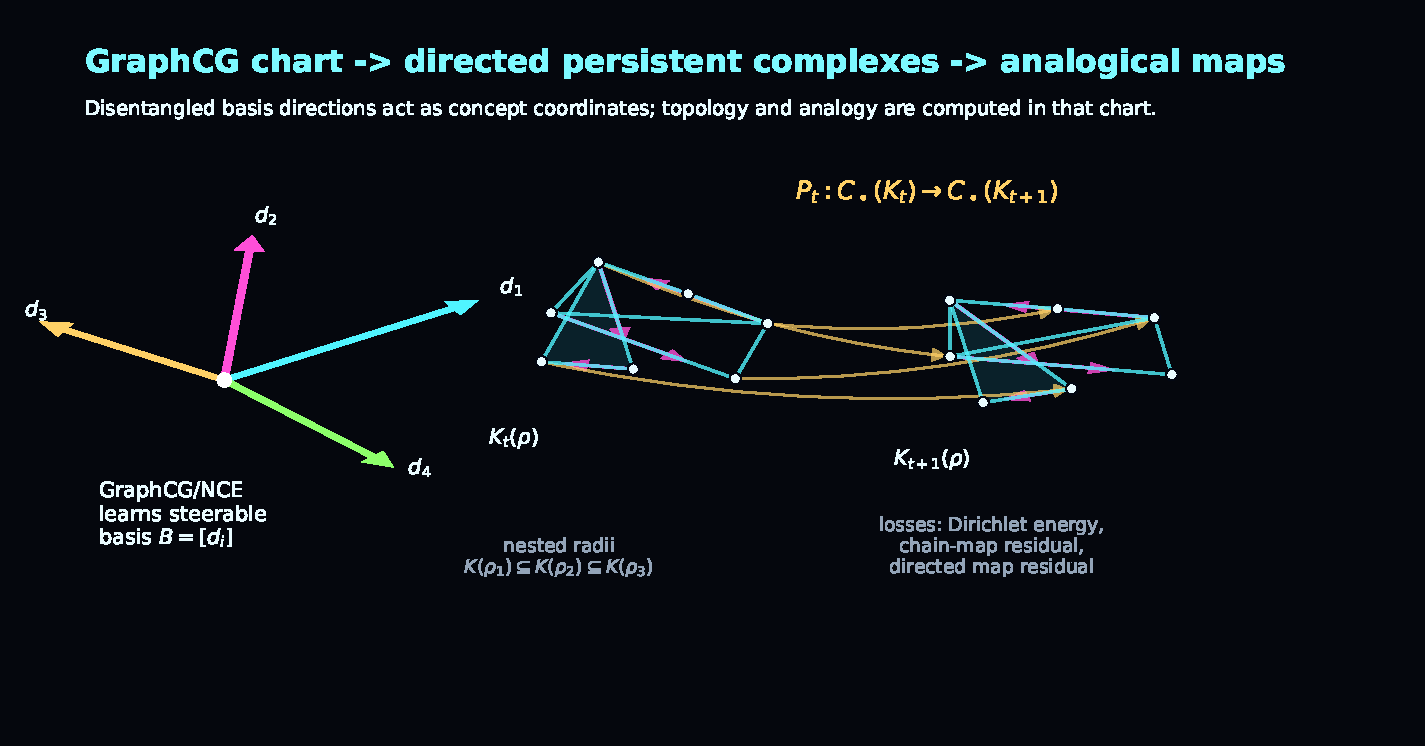
\includegraphics[width=\textwidth]{fig_graphcg_topology_analogy_map.pdf}
  \caption{GraphCG supplies a steerable concept chart; ToricGT builds directed persistent complexes in that chart and learns soft analogical maps between local reasoning complexes.  The maps are functor-like, but they also carry filtered simplicial, chain-map, and persistence-module structure.}
  \label{fig:graphcg-topology-analogy}
\end{figure}

\begin{definition}[Exact small persistence-module morphism audit]
For sampled analysis windows, replace the soft adjacencies by hard thresholded flag complexes over $\mathbb F_2$ up to dimension $2$.  Let $C_p(K_s(\rho_\ell))$ be the $p$-chain group and $\partial_p$ the boundary.  A nearest-neighbor vertex map induced by $P_s$ is accepted at target radius $\rho_{\ell'}$ if every source edge and triangle maps either to a collapsed simplex or to an edge or triangle in $K_{s+1}(\rho_{\ell'})$.  It then induces chain maps $F_{p,\ell,\ell'}$ and homology maps
\begin{equation}
  (F_{p,\ell,\ell'})_*:
  H_p(K_s(\rho_\ell);\mathbb F_2)
  \longrightarrow
  H_p(K_{s+1}(\rho_{\ell'});\mathbb F_2).
\end{equation}
The audit reports $\dim H_0$, $\dim H_1$, the ranks of $(F_0)_*$ and $(F_1)_*$, the minimal radius shift $\ell'-\ell$ required for a simplicial map, edge and triangle validity, directed-edge validity, and whether the complex was truncated for tractability.
\end{definition}

\begin{proposition}[Chain-map validity implies a homology map]
If $F_{p,\ell,\ell'}$ satisfies
\begin{equation}
  \partial_{p}^{s+1}F_{p,\ell,\ell'}=
  F_{p-1,\ell,\ell'}\partial_p^s,
\end{equation}
then it induces a well-defined linear map on $H_p$ over $\mathbb F_2$.
\end{proposition}

\begin{proof}
If $z\in C_p(K_s)$ is a cycle, then $\partial_p^s z=0$.  The chain-map identity gives
\begin{equation}
  \partial_p^{s+1}F_pz=F_{p-1}\partial_p^s z=0,
\end{equation}
so cycles map to cycles.  If $z$ and $z'$ differ by a boundary, $z-z'=\partial_{p+1}^s w$, then
\begin{equation}
  F_pz-F_pz'=F_p\partial_{p+1}^s w=\partial_{p+1}^{s+1}F_{p+1}w,
\end{equation}
so their images differ by a boundary.  Therefore the map depends only on homology classes.
\end{proof}

\begin{proposition}[Persistence stability for analogy filtrations]
Let $d$ and $\widehat d$ be two symmetric distance matrices on the same relation arrows, and let $\operatorname{Dgm}_p(d)$ and $\operatorname{Dgm}_p(\widehat d)$ be the degree-$p$ persistence diagrams of their Vietoris--Rips filtrations.  Then the bottleneck distance obeys
\begin{equation}
  d_B(\operatorname{Dgm}_p(d),\operatorname{Dgm}_p(\widehat d))
  \le \norm{d-\widehat d}_\infty.
\end{equation}
Consequently, small perturbations of hidden relation arrows cannot arbitrarily change the persistent homology unless they close or open a small-margin topological feature.
\end{proposition}

\begin{proof}
If $\norm{d-\widehat d}_\infty\le\eta$, then every edge present in the Rips complex of $d$ at radius $\rho$ is present in the Rips complex of $\widehat d$ at radius $\rho+\eta$, and conversely with $d$ and $\widehat d$ exchanged.  Thus the two filtrations are $\eta$-interleaved.  The algebraic stability theorem for persistence diagrams then gives the bottleneck bound \cite{cohensteiner2007stability,chazal2016structure}.  The final claim follows because a topological feature whose birth-death margin is larger than $2\eta$ cannot be removed by such a perturbation.
\end{proof}

The implementation uses differentiable proxies rather than a heavy persistent-homology dependency.  It logs inclusion residuals
\begin{equation}
  \mathcal L_{\mathrm{inc}}=\sum_{\ell<L}\norm{\max(0,A_\ell-A_{\ell+1})}_F^2,
\end{equation}
chain-map commutators for row-normalized prolongations $P_\ell$,
\begin{equation}
  \mathcal L_{\mathrm{chain}}=\sum_{\ell<L}\norm{P_{\ell+1}P_\ell-P_\ell P_{\ell+1}}_F^2,
\end{equation}
soft triangle density $\sum_{ijk}A_{ij}A_{jk}A_{ik}$, directed transitive residuals, and directed cycle/holonomy flux
\begin{equation}
  \Phi_\ell^\rightarrow
  =\sum_{i,j,k}A_\ell^\rightarrow(i,j)
  A_\ell^\rightarrow(j,k)A_\ell^\rightarrow(k,i)
  \max(0,\Omega_{ij})\max(0,\Omega_{jk})\max(0,\Omega_{ki}).
\end{equation}

\subsection{DEC conservative reasoning flow}

The directed simplicial layer also admits a conservative-flow interpretation inspired by discrete exterior calculus (DEC) discretizations of incompressible Navier--Stokes equations on simplicial surface meshes \cite{mohamed2016dec}.  Mohamed, Hirani, and Samtaney rewrite the continuous equations using exterior derivative, Hodge star, wedge product, and interior product, then replace these operators by DEC analogues.  The central lesson for ToricGT is not to simulate a fluid, but to audit whether a discrete trajectory respects conservative algebraic identities beyond pointwise prediction loss.  In the DEC paper, mass and vorticity conservation and kinetic-energy behavior reveal physical fidelity of the discretization; in ToricGT, analogous quantities reveal whether graph-of-thought hidden flows are organized or merely oscillatory.

For a local reasoning window at radius $\rho_\ell$, let $A_\ell^\rightarrow\in[0,1]^{n\times n}$ be the directed adjacency and set
\begin{equation}
  u_\ell=A_\ell^\rightarrow-(A_\ell^\rightarrow)\transpose .
\end{equation}
This antisymmetric matrix is treated as a discrete 1-form on the directed 1-skeleton.  Its divergence proxy is
\begin{equation}
  (\delta u_\ell)_i=\frac1{n-1}\sum_{j}u_\ell(i,j),
  \qquad
  \mathcal L_{\mathrm{mass}}(\ell)=\frac1n\sum_i(\delta u_\ell)_i^2.
\end{equation}
Low mass residual means that the local reasoning flow is not creating or destroying hidden-state mass at a vertex merely because the filtration radius changed.  Define a node circulation proxy
\begin{equation}
  \omega_{\ell,i}
  =
  \frac{\sum_j A_\ell(i,j)u_\ell(i,j)}
       {\sum_j A_\ell(i,j)+\epsilon},
\end{equation}
where $A_\ell$ is the symmetric adjacency.  The vorticity drift across adjacent radii is
\begin{equation}
  \mathcal L_{\omega}(\ell)=\norm{\omega_\ell-\omega_{\ell-1}}_2^2/n.
\end{equation}
The edge-flow kinetic energy is
\begin{equation}
  E_\ell=\frac{\sum_{ij}A_\ell(i,j)u_\ell(i,j)^2}{\sum_{ij}A_\ell(i,j)+\epsilon},
  \qquad
  \mathcal L_E(\ell)=(E_\ell-E_{\ell-1})^2.
\end{equation}
To mimic the metric role of the Hodge star, the implementation uses the HDBSCAN core radii as a diagonal dual-volume proxy,
\begin{equation}
  H_{ij}=\frac{(c_i+c_j+\epsilon)^{-1}}
              {\operatorname{mean}_{p\ne q}(c_p+c_q+\epsilon)^{-1}},
  \qquad
  E_\ell^\star=
  \frac{\sum_{ij}H_{ij}A_\ell(i,j)u_\ell(i,j)^2}
       {\sum_{ij}H_{ij}A_\ell(i,j)+\epsilon}.
\end{equation}
The Hodge-balance residual is
\begin{equation}
  \mathcal L_\star(\ell)=\left(E_\ell^\star/(|E_\ell|+\epsilon)-1\right)^2.
\end{equation}
Finally, the DEC convective term in the paper motivates a wedge/interior-product consistency check.  With average edge vorticity $\overline\omega_{ij}=(\omega_i+\omega_j)/2$, define
\begin{align}
  (u\wedge\omega)_{ij} &= u_{ij}\overline\omega_{ij},\\
  (i_u\omega)_{ij} &= A^\rightarrow_{ij}\omega_j-A^\rightarrow_{ji}\omega_i,
\end{align}
and penalize
\begin{equation}
  \mathcal L_\wedge(\ell)
  =
  \frac{\sum_{ij}A_\ell(i,j)\left((u\wedge\omega)_{ij}-(i_u\omega)_{ij}\right)^2}
       {\sum_{ij}A_\ell(i,j)+\epsilon}.
\end{equation}
The DEC conservative auxiliary is
\begin{equation}
  \mathcal L_{\mathrm{DEC}}
  =
  \mathcal L_{\mathrm{mass}}
  +0.25\mathcal L_\omega
  +0.10\mathcal L_E
  +0.05\mathcal L_\star
  +0.05\mathcal L_\wedge .
\end{equation}
It enters only as a small part of the step-topology loss.  The intended healthy regime is not zero directed flow: it is low divergence, bounded vorticity and kinetic drift, nonzero but stable directed cycle structure, and no domination of the BPB objective by a geometric auxiliary.

\begin{figure}[t]
  \centering
  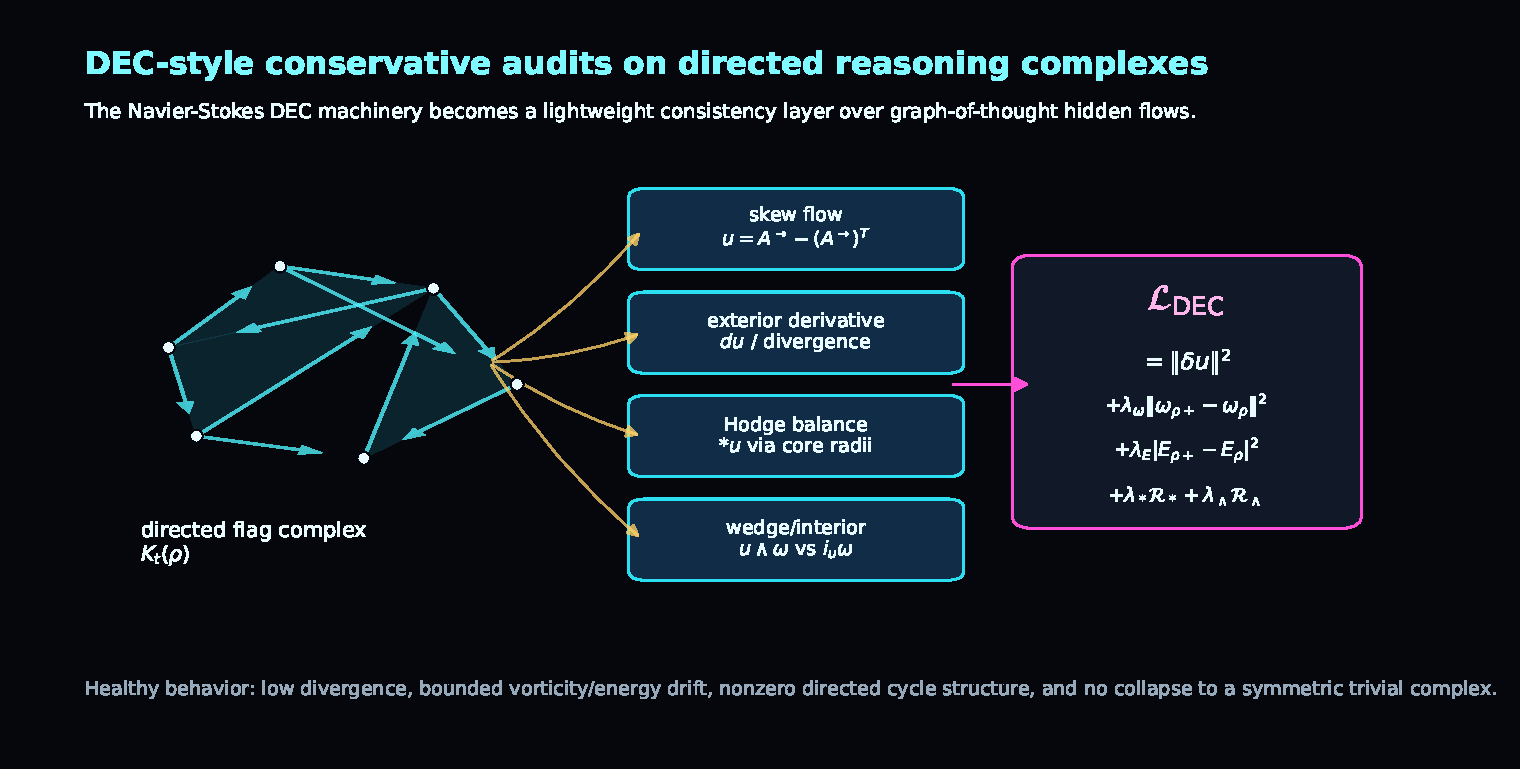
\includegraphics[width=\textwidth]{fig_dec_conservative_reasoning.pdf}
  \caption{DEC-inspired conservative audits for graph-of-thought reasoning.  A directed local reasoning complex supplies a discrete 1-form; divergence, circulation, Hodge-weighted energy, and wedge/interior consistency become finite diagnostics and low-weight training signals.}
  \label{fig:dec-conservative-reasoning}
\end{figure}

The latest training branch also adds a radius-parametrized HDBSCAN surrogate \cite{campello2013density,campello2015hierarchical,mcinnes2017hdbscan}.  For each relation class, let $c_i$ be the $k$th-nearest-neighbor core distance of $a_i$ and define the mutual-reachability distance
\begin{equation}
  d_{\mathrm{mr}}(i,j)=\max\{c_i,c_j,d_{ij}\}.
\end{equation}
Across the same radii $\rho_\ell$, define persistent density affinities
\begin{equation}
  H(i,j)=\frac1L\sum_{\ell=1}^L
  \sigma\left(\frac{\rho_\ell-d_{\mathrm{mr}}(i,j)}{\tau}\right)(1-\delta_{ij}).
\end{equation}
The auxiliary loss uses detached high-stability affinities as weights,
\begin{equation}
  \mathcal L_{\mathrm{HDB}}
  =
  \frac{\sum_{i\ne j} w_{ij}d_{ij}^2}{\sum_{i\ne j}w_{ij}+\epsilon},
  \qquad
  w_{ij}=\left[\max(0,H(i,j)-\alpha)\right]^2
  \mathbf 1\{s_i\ge m-1,\ s_j\ge m-1\},
\end{equation}
where $s_i=\sum_jH(i,j)$ is a density-stability score and $m$ is the minimum cluster size.  The detachment of $w_{ij}$ is intentional: persistent density neighborhoods may pull together, but unstable or outlier arrows do not receive gradients that would collapse unrelated analogies.  Periodic analyses compute the corresponding hard radius sweep, stable-cluster counts, outlier fractions, mutual-reachability heatmaps, and density-persistence adjacency plots.  Thus HDBSCAN is used as a relevance gate for the topology loss, not as an extra non-differentiable optimizer inside backpropagation.

\begin{proposition}[Scale stability of normalized analogy filtrations]
If all hidden arrows in one relation class are multiplied by a common scalar $\lambda>0$, then $d_{ij}$ is unchanged.  Consequently the symmetric filtration $\{A_\ell\}$ and every diagnostic depending only on $d_{ij}$ is invariant up to numerical $\epsilon$ effects.  If both channel blocks in $\Omega$ are normalized before forming the skew matrix, the directed filtration is also invariant to the same common rescaling.
\end{proposition}

\begin{proof}
The numerator $\norm{\lambda a_i-\lambda a_j}_2$ and the median denominator are both multiplied by $\lambda$, so their ratio is unchanged.  Therefore each logit $(\rho_\ell-d_{ij})/\tau$ is unchanged, and so is $A_\ell$.  The inclusion, chain-map, barcode-proxy, and triangle diagnostics are deterministic functions of these adjacencies.  For the directed case, normalized channel blocks satisfy $\lambda a_i^{(r)}/\norm{\lambda a_i^{(r)}}=a_i^{(r)}/\norm{a_i^{(r)}}$ for $\lambda>0$, so $\Omega_{ij}$ is unchanged.  Hence $A_\ell^\rightarrow$ and the directed diagnostics are unchanged as well.
\end{proof}

The noncommutative toric memory shapes the same trajectories through irrational phase probes.  In the compact Parameter-Golf adapter, target positions receive phase features
\begin{equation}
  (\sin 2\pi\theta t,\cos 2\pi\theta t,\sin 2\pi\beta t,\cos 2\pi\beta t),
\end{equation}
and memory slots carry a finite cocycle-like phase
\begin{equation}
  \chi_s=\exp\bigl(2\pi i(\theta s^2+\beta s)\bigr).
\end{equation}
When $1,\theta,\beta$ are rationally independent, the projected path
\begin{equation}
  \Pi(t)=((R+r\cos 2\pi\beta t)\cos 2\pi\theta t,\,
  (R+r\cos 2\pi\beta t)\sin 2\pi\theta t,\,
  r\sin 2\pi\beta t)
\end{equation}
is pseudo-periodic and equidistributed on the visualization torus in the finite-prefix sense.  This does not by itself solve reasoning; it supplies a nonrepeating phase scaffold that helps separate random-order positions, exposes recurrence, and contributes an antisymmetric skew term to directed topology diagnostics.

\begin{figure}[t]
  \centering
  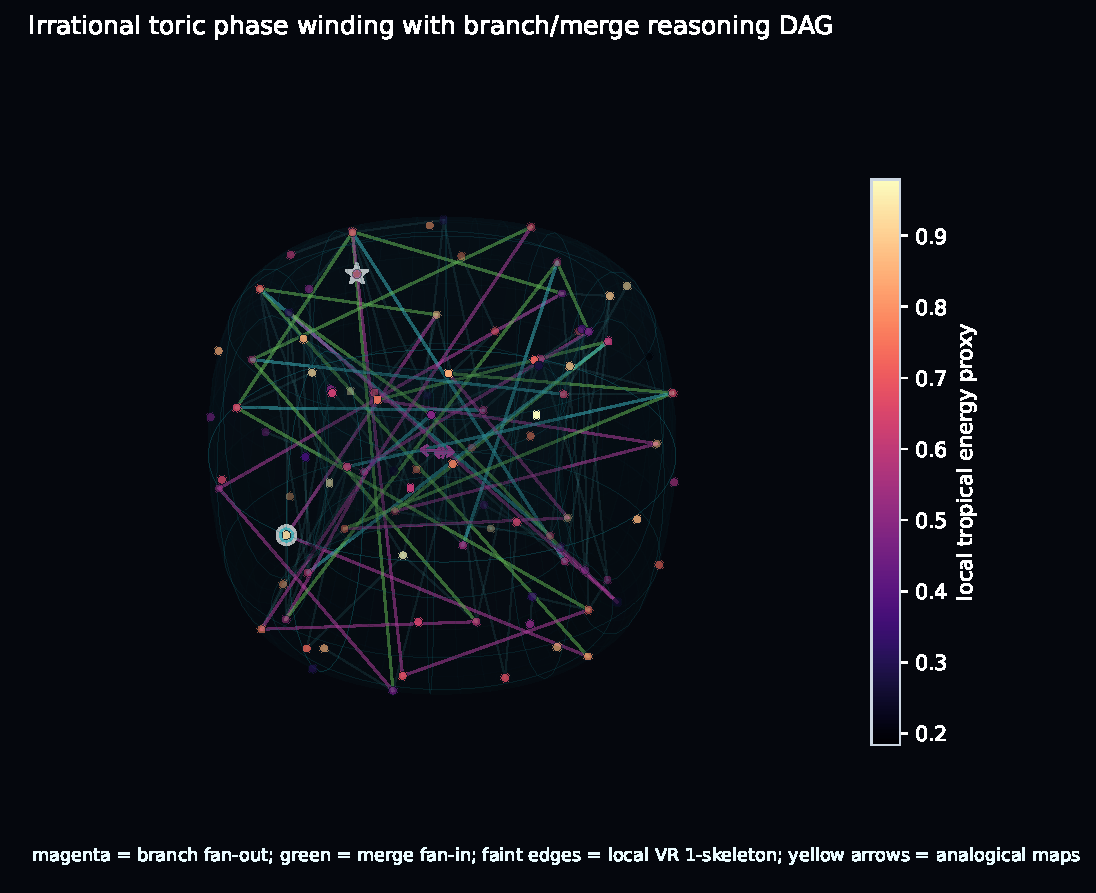
\includegraphics[width=0.92\textwidth]{fig_toric_phase_simplicial_trajectory.pdf}
  \caption{Irrational toric phase projection of a branch/merge reasoning DAG.  Vertices lie on a nonrepeating toric phase scaffold; local Vietoris--Rips edges reveal step-level simplicial structure; colored directed edges distinguish branch fan-out, merge fan-in, and analogical transport.}
  \label{fig:toric-phase-simplicial}
\end{figure}

Periodic analyses render these quantities directly.  For selected reasoning records the script writes branch counts, merge counts, branch diversity, merge scatter, back-edge fraction, induced edge/triangle simplex densities, directed filtration curves for edge density, triangle density, asymmetry, cycle flux, DEC conservation residuals, and mass residuals; heatmaps of normalized distances, mutual reachability, the antisymmetric toric skew matrix, and directed adjacencies; window-by-radius simplex hierarchy plots with DEC kinetic and wedge/interior panels; exact $\mathbb F_2$ persistence-module morphism heatmaps for $H_0$ and $H_1$; and toric phase/simplicial DAG plots.  Thus the noncommutative topology is both a training pressure and an auditable explanation object.

\begin{proposition}[Dense recurrent blocks are the byte-efficient default]
Under a strict serialized-byte cap, replacing a dense feed-forward block of size $O(dd_{\mathrm{ff}})$ by $E$ full experts costs $O(Edd_{\mathrm{ff}})$ stored scalars, whereas applying the same dense block recurrently $r$ times costs no additional stored scalars.  Therefore the Parameter-Golf default should be dense recurrent ToricGT blocks, with Soft-MoE retained as a measured ablation or low-rank adapter variant.
\end{proposition}

\begin{proof}
The artifact stores parameters, tokenizer, code, and metadata, not floating-point operations.  A full expert bank serializes $E$ separate MLP parameter sets.  A recurrent dense block serializes one MLP parameter set and increases only runtime.  When the cap is binding and the evaluator allows a fixed training/evaluation program, recurrent dense computation has a better first-order byte/computation tradeoff.  Soft-MoE becomes attractive only if low-rank adapters or routing vectors improve BPB enough to justify their extra bytes.
\end{proof}

\subsection{Micro-ToricGT language-model design}

The contest model should be a language model inspired by ToricGT, not the full graph-to-graph encoder.  The recommended design is:
\begin{enumerate}[leftmargin=2em]
  \item a byte-level tokenizer with tied input/output embeddings;
  \item randomized content-independent target-position order by default;
  \item a small number of dense unique Transformer blocks reused recurrently to increase effective depth without storing more block parameters;
  \item lower softmax layers and upper tropical-ring layers with stabilized score normalization and residual gates;
  \item fixed toric phase features of target positions and optional PolarQuant KV perturbation audits;
  \item a compact prefix-visible GFlowNet action policy for latent graph-of-thought sampling;
  \item compact serialization of \texttt{graph\_json} node/edge records into the byte stream, so graph-structured supervision is not discarded in the contest adapter;
  \item final int8 export by default, with int6/int4 packing tested only after round-trip BPB checks;
  \item optional Soft-MoE or low-rank expert adapters only as byte-accounted ablations after a dense baseline is stable.
\end{enumerate}

A safe starting microarchitecture for the implemented dense track is
\begin{equation}
  V=260,\quad d=384,\quad H=6,\quad
  L_{\mathrm{unique}}=7,\quad L_{\mathrm{effective}}=14,
\end{equation}
with tied embeddings, recurrent block tying, hybrid softmax/tropical-ring attention, a tiny $A=8$ action GFlowNet policy, and no stored expert bank.  In the current artifact audit this gives about $13.0$M stored scalars and an int8 compressed artifact around $12.94$MB, leaving margin below $16{,}000{,}000$ bytes for code and metadata.  If $P_{\mathrm{fp}}$ is the uncompressed scalar count, then int8 export roughly permits $P_{\mathrm{fp}}<16$M minus code overhead; int6 export roughly permits $P_{\mathrm{fp}}<21$M before entropy compression; int4 export permits more parameters but is less stable unless quantization-aware training is strong.  These are engineering estimates; the actual gate is the serialized artifact size.

For experimental triage, report BPB with matched seeds, validation byte counts, exported-artifact round-trip checks, and confidence intervals.  Single-run changes below the measured seed-to-seed variation should be treated as noise, even if the auxiliary diagnostics improve.  A Toric BGG component earns its place in the compressed model only when it improves BPB after export or produces a predeclared reasoning improvement without a BPB regression.

\begin{proposition}[Depth recurrence improves effective computation without increasing stored block parameters]
Let a block $\Psi_\theta$ be applied $r$ times with shared parameters.  The stored parameter count is $|\theta|$, while the effective computational depth is $r$.  If $\Psi_\theta$ is token equivariant, then $\Psi_\theta^r$ is token equivariant.
\end{proposition}

\begin{proof}
Only one copy of $\theta$ is serialized, so stored parameters do not scale with $r$.  The composition of $r$ copies of the same equivariant map is equivariant because for any permutation $P$,
\begin{equation}
  \Psi_\theta^r(PX)=\Psi_\theta^{r-1}(P\Psi_\theta(X))=P\Psi_\theta^r(X)
\end{equation}
by induction.
\end{proof}

\subsection{Soft-MoE under a 16 MB artifact cap}

A naive Soft-MoE can violate the artifact budget because it stores multiple expert MLPs.  The contest adaptation must use one or more of the following parameter-sharing schemes.
\begin{enumerate}[leftmargin=2em]
  \item \textbf{Shared base plus expert adapters}: $f_e(x)=f_0(x)+B_e\sigma(A_e x)$ with small rank $r\ll d$.
  \item \textbf{Tied expert matrices}: all experts share $W_1,W_2$ but have expert-specific gates, biases, or low-rank deltas.
  \item \textbf{Grouped experts}: experts are reused across recurrent layers and only routing vectors $\Phi$ change by layer.
  \item \textbf{Quantized experts}: expert weights are trained with straight-through quantization and exported in int6/int8.
  \item \textbf{Pruned slots}: keep $E S\le8$ or $16$ for the contest model; large slot counts are inappropriate under the wallclock cap.
\end{enumerate}

For a low-rank expert adapter with rank $r$, the incremental parameter cost per expert is approximately
\begin{equation}
  P_{\mathrm{adapter}}\approx 2dr+2d_{\mathrm{ff}}r+O(d+d_{\mathrm{ff}}),
\end{equation}
which is far smaller than a full expert cost $2dd_{\mathrm{ff}}$.  Therefore a Parameter-Golf Soft-MoE block should store one shared dense MLP plus small expert adapters.  The graph-reasoning version may use full typed experts; the contest version should not unless artifact measurements prove it fits.

\subsection{Distillation from ToricGT to the contest LM}

The full ToricGT model can help the contest track before submission by producing training-time supervisory signals.  The contest artifact should not need the teacher at evaluation.  Let $p_T$ be a trained ToricGT-derived teacher distribution over serialized graph-reasoning traces and $p_S$ be the micro language model.  A compliant training objective on allowed training data is
\begin{equation}
  \mathcal L_{\mathrm{PG}}=\mathcal L_{\mathrm{LM}}
  +\lambda_{\mathrm{KD}}T^2\operatorname{KL}\left(p_T^{(T)}(\cdot\mid c)\;\Vert\;p_S^{(T)}(\cdot\mid c)\right)
  +\lambda_h\norm{R h_T-h_S}_2^2
  +\lambda_q\mathcal L_{\mathrm{QAT}},
\end{equation}
where $c$ ranges over training contexts, $T$ is distillation temperature, $R$ is a small learned projection used only during training, and $\mathcal L_{\mathrm{QAT}}$ is the quantization-aware training loss.  Teacher logits, if stored, must be generated from allowed training data and must not be used as hidden validation information.  In the final artifact, omit the teacher, omit distillation heads, and serialize only the student.


\subsection{Artifact packing and runtime implementation}

A robust contest script should separate training-time tensors from serialized tensors.  During training, keep fp16 or bf16 master weights and fake-quantized forward weights.  At export, pack only the deployable state:
\begin{equation}
  \mathcal A=\operatorname{Pack}\left(\operatorname{Quantize}(\theta_S),\operatorname{Tokenizer},\operatorname{Config},\operatorname{DecodeCode}\right).
\end{equation}
The export test is not complete until the model is loaded from $\mathcal A$ and evaluated without the floating-point training checkpoint.  The following checks should be hard failures in \texttt{train\_gpt.py}:
\begin{verbatim}
assert artifact_bytes <= 16_000_000
assert not uses_network()
assert not reads_validation_except_eval_stream()
assert roundtrip_bpb_close(float_eval_bpb, packed_eval_bpb, tolerance=0.01)
assert causal_audit_passed(model)
\end{verbatim}
The size audit should report at least
\begin{equation}
  (B_{\mathrm{code}},B_{\mathrm{weights}},B_{\mathrm{tokenizer}},B_{\mathrm{metadata}},B_{\mathrm{art}}),
\end{equation}
and the log should include the exact command, seed, git commit, wallclock, GPU type, tokenizer, vocabulary size, number of unique blocks, recurrence depth, number of Soft-MoE experts, slots per expert, quantization bits, validation BPB, and validation bytes.  For a ToricGT-derived model, also report whether causal Soft-MoE, toric adapters, tropical gates, or teacher distillation were active.

\subsection{Contest record folder checklist}

A ToricGT Parameter-Golf submission should create a record folder with:
\begin{verbatim}
records/<name>/
  README.md              # architecture, training recipe, size accounting
  submission.json        # author, GitHub id, val_bpb, metadata
  train.log              # automatic training/eval log, preferably 3 seeds
  train_gpt.py           # self-contained runnable script
  requirements.txt       # only if extra packages are needed
\end{verbatim}
Before opening a pull request, run:
\begin{verbatim}
python train_gpt.py --dry_run_size_check
python train_gpt.py --minimal_train_check --max_steps 20
python train_gpt.py --roundtrip_quantize
python train_gpt.py --eval_only --assert_no_network
\end{verbatim}
The script should print train loss, validation loss, validation BPB, compressed model bytes, code bytes, artifact bytes, seed, wallclock, and hardware.  The size check must compute decimal bytes and fail at $16{,}000{,}000$, not $16$ MiB.

\subsection{Pragmatic risk controls}

The Parameter-Golf track has different failure modes from the research model.  The most important controls are:
\begin{enumerate}[leftmargin=2em]
  \item keep a boring dense baseline in the record folder before adding Soft-MoE;
  \item measure artifact bytes after every architecture change;
  \item verify quantized round-trip evaluation, not only floating-point evaluation;
  \item maintain three-seed evidence before claiming a record-quality result;
  \item keep validation handling strictly score-first and never train on future validation tokens;
  \item prefer self-contained torch code over fragile external imports, even if imports are nominally allowed;
  \item document every compression, tokenizer, and test-time adaptation trick in the README.
\end{enumerate}
The contest leaderboard shows that successful submissions often combine small-model architecture changes, quantization, recurrent or parallel residual computation, tokenizer/data transforms, and legal test-time adaptation.  ToricGT should borrow these tactics only when they are compatible with the self-contained artifact and validation rules.


\subsection{Checkpoint triage and activation gates}\label{subsec:checkpoint-triage}

A ToricGT training run should be controlled by gates rather than by enthusiasm for auxiliary structure.  The deployable candidate for a BPB-constrained track is a dense or lightly adapted autoregressive model; the full graph model is the teacher and diagnostic scaffold.  Training-only toric, GraphCG, BGG, Slepian, topology, and multi-token-head probes are enabled only when they pass three checks: the validation BPB trend is nondegrading, the exact small-window algebraic audit agrees with the differentiable surrogate, and the ablation improves at least one predeclared reasoning metric.

The conservative recovery mode is
\begin{equation}
  \lambda_{\mathrm{TBGG}}=\lambda_{\mathrm{EulerKoszul}}=\lambda_{\mathrm{flow}}=\lambda_{\mathrm{QAT}}=0,
  \qquad 0<\lambda_{\mathrm{GFN}},\lambda_{\mathrm{GraphCG}}\ll1,
\end{equation}
with tighter gradient clipping and no new deployable parameters.  Toric BGG losses are activated in the following order: $\partial^2$ residual, standard-filtration leakage, signature distillation, Gale-dual consistency, and Euler-Koszul exactness.  This order reflects numerical conditioning.  The first two losses are local and sparse; the last two require the representation to have already stabilized.

The gate writes an audit record containing validation BPB, answer-span BPB, branch-search lift, graph-answer accuracy, resolution-consistency score, standard-filtration leakage, Koszul-linearity residual, Gale-dual consistency, BGG trajectory retrieval at $K$, GraphCG covariance, tropical active-face margins, and artifact bytes after round-trip export.  A run may continue with a larger Toric BGG weight only if the record shows no score-first violation and no statistically meaningful BPB regression relative to a matched seed or matched checkpoint window.

In the current implementation this audit is made explicit by a BPB-transfer controller.  For each family $f$ in
\[
  \{\mathrm{BGG/Koszul},\mathrm{topology},\mathrm{toric},\mathrm{tropical},
  \mathrm{Slepian/Pollak},\mathrm{GraphCG},\mathrm{memory},\mathrm{analogy}\},
\]
the controller records pressure $p_f$, recent held-out BPB transfer $\Delta_f$, artifact-size risk $a$, and the current phase $s$.  Before the threshold checkpoint,
\[
  \lambda_f =
  \begin{cases}
    \epsilon_f & \text{if } \Delta_f>0 \text{ with sufficient evidence and } a<1,\\
    0 & \text{otherwise,}
  \end{cases}
\]
while the BPB objective keeps weight one.  Thus attractive algebraic or topological plots are not allowed to redirect the competition optimizer unless they first show predictive transfer to validation BPB.  After a protected $\le1.2$ artifact exists, the same controller can promote these families into the graph-of-thought, GFlowNet, memory, analogical, and long-context phases.
\section{Datasets, synthetic families, and leakage control}

\subsection{Training mixture}

The data plan is graph-first.  Every raw record is normalized into a graph record with question, answer, reasoning, metadata, stable hashes, graph JSON, token-count estimates, and deterministic split fields.  The local curation plan targets chain-of-thought, tree-of-thought, graph-of-thought, mathematical, programming, OpenAI-origin GSM8K, Hebrew morphology, rabbinic Hebrew/Aramaic-English, and Jewish Hebrew text sources.  It writes Parquet outputs and split reports suitable for training and, after license review, possible Hugging Face upload.

{\small
\begin{longtable}{>{\raggedright\arraybackslash}p{0.24\linewidth}>{\raggedright\arraybackslash}p{0.24\linewidth}>{\raggedright\arraybackslash}p{0.14\linewidth}>{\raggedright\arraybackslash}p{0.27\linewidth}}
\toprule
Dataset & Selected loader/config & License observed & ToricGT role \\
\midrule
\endhead
NuminaMath-CoT & default via \texttt{datasets} & Apache-2.0 & large math CoT to proof graphs \\
OpenR1-Math-220k & \texttt{all} via \texttt{datasets} & Apache-2.0 & multi-trace math reasoning \\
Codeforces-CoTs & decontaminated Python/editorial config & CC-BY-4.0 & algorithmic/programming CoT \\
GSM8K & \texttt{main} & MIT & OpenAI math word problems \\
Hendrycks MATH & seven subject configs & MIT & competition math and verifier checks \\
MATH-500 & default/test & dataset card & verifier-style benchmark \\
Tree-of-Thoughts 24k & raw JSON & Apache-2.0 & explicit ToT branches \\
Got Math 500K & raw JSONL stream & Apache-2.0 & explicit GoT math \\
UniMorph Hebrew & raw UniMorph TSV fallback & CC-BY-SA-3.0 & Hebrew lemma/inflection graphs \\
Sefaria parallel pairs & default & CC-BY-4.0 & rabbinic Hebrew/Aramaic-English parallel text \\
Sefaria Hebrew library & default & GPL-3.0 & large Jewish Hebrew text library \\
Superior-Reasoning gpt-oss & \texttt{stage1}/\texttt{stage2} & CC-BY-4.0 & frontier open-weight reasoning distillation \\
GPT-OSS math distill & default & Apache-2.0 & gpt-oss math rationales \\
Algorithmic SFT v1 & default & MIT & procedural algorithmic traces \\
Graph reasoning messages & default & Apache-2.0 & graph-structured reasoning dialogue \\
DAG reasoning & default & Apache-2.0 & dependency-aware reasoning traces \\
Opus reasoning 24k & default & Apache-2.0 & high-quality reasoning style transfer \\
\bottomrule
\end{longtable}
}

The important loader details are pragmatic.  The UniMorph Hub repository may contain an old dataset script, so the Hebrew file should be downloaded directly from the UniMorph GitHub source when the current \texttt{datasets} package rejects the script.  The GoT and ToT sources are raw JSON/JSONL rather than conventional multi-shard builders, so the curation script downloads and streams them directly.  The Hebrew/Jewish-text slice intentionally uses Sefaria and UniMorph Hebrew sources rather than Christian-branded biblical-language datasets when the experimental goal is Jewish Hebrew/rabbinic coverage.

Hebrew rows are niqqud-aware.  The curation policy is to preserve pointed Hebrew when the upstream source provides it, prefer same-consonant pointed variants when an equivalent field is present, and explicitly flag unpointed Hebrew rather than synthesize vowels into attested source text.  The current audit finds $3{,}564{,}756$ rows containing Hebrew, of which $2{,}868$ are pointed upstream rows and $3{,}561{,}888$ are unpointed upstream rows.  Strict pointed-Hebrew runs should filter out records with \texttt{has\_hebrew\_without\_niqqud=true}; broader Jewish-text pretraining can retain them while making the missing-vowel status visible to the model and to evaluation reports.

\subsection{Normalized record schema}

Every curated row should contain:
\begin{verbatim}
record_id, dataset, config, source_split, source_index,
task_family, language, license, role,
question, answer, solution, reasoning,
metadata_json, text, graph_json,
content_hash, group_hash, split,
estimated_tokens, quality_flags_json
\end{verbatim}
The schema separates the human-readable training view from the graph view.  The \texttt{text} field supports ordinary language-model distillation and debugging; the \texttt{graph\_json} field supports TokenGT conversion, graph-to-graph prediction, GFlowNet state construction, and visualization.

\subsection{Graph conversion policy}

The conservative base graph has a \texttt{problem} node, zero or more \texttt{reasoning\_step} nodes, an \texttt{answer} node, \texttt{depends\_on} edges between consecutive or referenced steps, and a \texttt{supports\_answer} edge from the final step or problem node to the answer node.  Dataset-specific additions are:
\begin{enumerate}[leftmargin=2em]
  \item Codeforces rows add \texttt{problem\_statement}, \texttt{editorial}, \texttt{public\_test}, and \texttt{code\_solution} nodes when available.
  \item OpenR1 rows add one generation node per sampled reasoning trace when multiple traces are present.
  \item UniMorph rows add \texttt{lemma}, \texttt{form}, and \texttt{features} nodes.
  \item Sefaria parallel rows add \texttt{ref}, \texttt{hebrew\_or\_aramaic}, \texttt{english}, and \texttt{category} nodes.
  \item Sefaria Hebrew-library rows add \texttt{ref}, \texttt{category}, \texttt{version}, and \texttt{text} nodes when metadata is available.
  \item ToT/GoT rows preserve branch markers and tag records as \texttt{tot} or \texttt{got\_math} for richer later conversion.
\end{enumerate}
This representation is deliberately conservative: it is sufficient for TokenGT pretraining and can be refined later without redownloading raw sources.

\subsection{Leakage-resistant splitting}

Random record-level splits are invalid for this setting.  Near-duplicate chain-of-thought traces, identical proof graphs, inverse braid words, conjugate torus words, repeated Hebrew lexeme paradigms, and copied Sefaria references can leak structure.

\begin{definition}[Leakage cluster]
A leakage cluster is an equivalence class generated by any of the following high-similarity relations: exact normalized-content hash, source-family key collision, text shingle SimHash prefix match, graph Weisfeiler-Lehman sketch match, algebraic normal-form equivalence, inverse/conjugate word equivalence, same Hebrew root paradigm, Sefaria reference identity, or graph-isomorphism equivalence for synthetic dynamic-programming instances.
\end{definition}

The practical splitter computes canonical text, exact \texttt{content\_hash}, task-family keys such as Codeforces problem id or Sefaria reference, and a stable SimHash prefix over word shingles.  The \texttt{group\_hash} combines task-family key, content hash, and SimHash prefix.  Split assignment is deterministic:
\begin{equation}
  \operatorname{split}(g)=
  \begin{cases}
  \text{train}, & h(g)\in[0,80),\\
  \text{validation}, & h(g)\in[80,90),\\
  \text{test}, & h(g)\in[90,100),
  \end{cases}
\end{equation}
where $h(g)$ is a stable hash percentile.  All rows with the same group key go to the same split.  For synthetic algebra, stronger family holdouts override percentile splitting: hold out denominator intervals $q$, word lengths, Coxeter ranks, graph sizes, root families, and root-template pairs.

\begin{proposition}[Cluster splitting prevents direct duplicate leakage]
If every leakage cluster is assigned wholly to one split, then no train/test pair is connected by the chosen leakage relations.
\end{proposition}

\begin{proof}
Assume for contradiction that a train record $r$ and a test record $s$ are connected by a leakage relation.  By definition, $r$ and $s$ lie in the same equivalence class generated by such relations.  Cluster splitting assigns the entire class to a single split, contradicting that $r$ is train and $s$ is test.
\end{proof}

\subsection{Output layout and commands}

The curation output should have the following structure.
\begin{verbatim}
data/
  curated/
    manifest.json
    split_report.json
    split_report.md
    all.parquet
    train.parquet
    validation.parquet
    test.parquet
    by_dataset/<safe_dataset_name>.parquet
  raw/hf/
    downloaded raw JSON/JSONL fallback files
\end{verbatim}
Run a full curation with:
\begin{verbatim}
conda run -n tokengt env PYTHONPATH=src python scripts/curate_datasets.py \
  --output-dir data/curated \
  --raw-dir data/raw/hf \
  --chunk-size 20000 \
  --num-workers 16 \
  --normalize-batch-size 256
\end{verbatim}
Run a bounded sample curation with:
\begin{verbatim}
conda run -n tokengt env PYTHONPATH=src python scripts/curate_datasets.py \
  --output-dir data/curated_sample \
  --raw-dir data/raw/hf \
  --max-records-per-source 1000 \
  --num-workers 4 \
  --normalize-batch-size 128
\end{verbatim}
Validate outputs with:
\begin{verbatim}
conda run -n tokengt env PYTHONPATH=src python scripts/inspect_curated_data.py \
  --curated-dir data/curated
\end{verbatim}
Use 8--16 CPU workers on a 32-thread workstation, lowering the count when other CPU-heavy jobs are running.  Large direct downloads can use \texttt{aria2c} when available, but the bottleneck is often Python-side graph normalization, SimHash grouping, and Parquet writing.

\subsection{Expected scale and license handling}

The first full pass is expected to produce about $5.2$M records: roughly $859$k NuminaMath, $225$k OpenR1, $500$k GoT Math, $9.8$k Codeforces, $8.8$k GSM8K, $12.5$k MATH, $24.7$k ToT, $3.55$M Sefaria Hebrew-library records, $3.7$k Sefaria parallel pairs, and a small UniMorph Hebrew table.  This is enough for the lower Chinchilla-style token budget for 8M-35M parameters once reasoning text, Hebrew text, and graph tokens are counted.

Before publishing any normalized data, re-check every license, preserve source attribution columns, and consider publishing only metadata and graph-conversion outputs where redistribution is allowed.  Do not publish records from sources whose terms prohibit redistribution or require gating.  GPL-licensed data, in particular, should be handled separately from permissively licensed training mixtures when downstream model or dataset release terms matter.

\subsection{Synthetic generator specifications}

\paragraph{Rotation words.}
Sample words in $\{U,U^{-1},V,V^{-1}\}$, reduce to $\omega^cU^aV^b$, and emit each rewrite as a graph edge labeled \texttt{commutes\_with\_phase} or \texttt{cancels}.  Hold out denominator intervals $q$, word lengths, and phase exponents.

\paragraph{Higher tori.}
Sample skew matrices $\Theta$ and words in $U_1^{\pm1},\ldots,U_n^{\pm1}$.  Targets include ordered exponent vector $a\in\Z^n$ and symbolic phase
\begin{equation}
  \exp\left(2\pi i\sum_{j<k}c_{jk}\Theta_{jk}\right).
\end{equation}

\paragraph{Hebrew roots.}
Sample root families and templates from curated lexica or analyzer outputs.  Create graph records with shared root nodes, radical nodes, template nodes, binyan nodes, and uncertain hypotheses.  Hold out entire roots or entire root-template combinations to test abstraction.

\paragraph{Tropical algorithms.}
Generate weighted graphs and full Bellman-Ford/Floyd-Warshall traces.  Record selected and dominated candidates, active faces, margins, and final distances.

\section{Model, losses, and training schedule}

\subsection{Architecture}

A practical 8M-35M parameter ToricGT family uses $L=6$--$12$ layers, width $d=256$--$512$, eight heads, MLP expansion four, softmax/hybrid lower layers, tropical ring middle and upper layers, node/edge/graph heads, optional Hebrew morphology heads, optional GFlowNet policy heads, default Soft-MoE feed-forward replacements in the upper half of the graph model, and optional PolarQuant cache at inference.  The full research model is graph-to-graph.  The Parameter-Golf variant is a dense random-order byte model with tied embeddings, recurrent blocks, target-position toric phases, stabilized tropical-ring attention, and byte-accounted quantized export.

The rough parameter count is
\begin{equation}
  P\approx L\left(4d^2+8d^2\right)+O(dV_{\mathrm{feat}}),
\end{equation}
where $4d^2$ is attention projection scale and $8d^2$ is a two-layer feed-forward block with expansion four.  Because graph-token feature vocabularies are small compared with language vocabularies, most parameters sit in the encoder.  If a dense feed-forward block is replaced by full Soft-MoE experts, the stored parameter count grows roughly like $E$ times the expert MLP size plus $dES$ router parameters.  For the research model this can be acceptable when $E$ is small.  For Parameter Golf, use shared experts or low-rank expert adapters so that increased specialization does not destroy the artifact budget.

\subsection{Composite objective}

The supervised objective is
\begin{equation}
\begin{split}
  \mathcal L_{\mathrm{sup}}={}&\lambda_V\mathcal L_V+\lambda_E\mathcal L_E+\lambda_G\mathcal L_G+
  \lambda_{\mathrm{eq}}\mathcal L_{\mathrm{eq}}+
  \lambda_\Theta\mathcal L_\Theta+\lambda_{\mathrm{trop}}\mathcal L_{\mathrm{margin}}\\
  &+\lambda_H(\mathcal L_{\mathrm{root}}+\mathcal L_{\mathrm{align}}+\mathcal L_{\mathrm{binyan}}+\mathcal L_{\mathrm{feat}}+\mathcal L_{\mathrm{par}})
  +\lambda_{\mathrm{moe}}\mathcal L_{\mathrm{moe}}
  +\lambda_{\mathrm{cache}}\mathcal L_{\mathrm{PQ}}
  +\lambda_{\mathrm{KD}}\mathcal L_{\mathrm{distill}}.
\end{split}
\end{equation}
The equivariance loss is
\begin{equation}
  \mathcal L_{\mathrm{eq}}=\Eop_{\pi}\norm{F(\pi G)-P_\pi F(G)}_2^2.
\end{equation}
The torus loss is
\begin{equation}
  \mathcal L_\Theta=\sum_{j<k}\norm{U_jU_kH-e^{2\pi i\Theta_{jk}}U_kU_jH}_F^2.
\end{equation}
A stable tropical objective combines margin and entropy:
\begin{equation}
  \mathcal L_{\mathrm{margin}}=-\Eop[\Delta_{\mathrm{correct}}]+\beta\Eop[\max(0,\Delta_{\mathrm{collapse}}-H(A))].
\end{equation}

\subsection{Schedule}

\begin{enumerate}[leftmargin=2em]
  \item \textbf{Phase A: implementation validation}.  CPU-only shape tests, equivariance tests, mask tests, and exact tropical ring-vs-full comparisons.
  \item \textbf{Phase B: synthetic algebra}.  Rotation words, finite tori, braid/Coxeter tasks, and tropical dynamic programming.
  \item \textbf{Phase C: curated reasoning graphs}.  Math, algorithmic, and Hebrew morphology graph records with clustered splits.
  \item \textbf{Phase D: GFlowNet fine-tuning}.  Activate trajectory or subtrajectory balance over embedding-space graph refinements.
  \item \textbf{Phase E: long-context cache evaluation}.  Enable PolarQuant cache for long graph-token traces and compare exact KV, unquantized ring, and polar ring cache.
  \item \textbf{Phase F: Parameter-Golf random-order compression}.  Train the dense random-order byte model with compact graph-json projection and prefix-visible GFlowNet action sampling, measure BPB and artifact bytes, add compact Soft-MoE adapters only if they improve BPB under the same cap, run quantization-aware or post-training export checks, and export a self-contained artifact with exact byte accounting.
\end{enumerate}

\section{Evaluation and ablations}

Core metrics include node accuracy/regression, edge accuracy/regression, graph answer exact match, proof validity, equivariance error, tropical margin and active-face entropy, torus commutator error, Hebrew root/binyan/feature F1, paradigm consistency, Soft-MoE expert utilization and slot entropy, Parameter-Golf artifact bytes and validation BPB for the micro-LM track, compact GFlowNet action entropy/diversity, GFlowNet reward calibration, terminal diversity, and OOD generalization over graph size, word length, denominator $q$, Coxeter rank, and Hebrew root families.

\begin{longtable}{p{0.32\linewidth}p{0.56\linewidth}}
\toprule
Ablation & Question answered \\
\midrule
\endhead
Softmax TokenGT, no toric features & Is graph tokenization alone sufficient? \\
Softmax TokenGT + toric features & Do phase channels help without tropical heads? \\
Tropical heads, no ring schedule & Does max-plus reasoning help independent of systems schedule? \\
Tropical ring heads & Does exact blockwise evaluation preserve quality at longer context? \\
No equivariance loss & Does architecture alone enforce enough symmetry in practice? \\
No torus regularizer & Are phase channels learned structurally or memorized? \\
No Hebrew graph factorization & Does root-template structure outperform string-only morphology? \\
GFlowNet token-space vs embedding-space & Which action space gives more diverse high-reward graphs? \\
Dense FFN vs Soft-MoE ToricGT & Does typed differentiable routing improve graph reasoning without destabilizing training? \\
Full expert Soft-MoE vs shared-adapter Soft-MoE & Which expert parameterization gives the best quality/byte tradeoff? \\
Full ToricGT vs micro-ToricGT LM & Which graph-reasoning inductive biases survive the Parameter-Golf compression regime? \\
Full KV vs PolarQuant cache & Does polar cache compression preserve long-context graph reasoning? \\
\bottomrule
\end{longtable}

\section{Implementation blueprint}

The codebase should be organized as follows.
\begin{enumerate}[leftmargin=2em]
  \item \texttt{typed\_graph.py}: graph schema, relabeling, canonicalization, masks.
  \item \texttt{graph\_tokenizer.py}: node, edge, endpoint, toric, Hebrew, and structural feature channels.
  \item \texttt{tropical\_attention.py}: full tropical attention, ring tropical attention, provenance, margins.
  \item \texttt{toric\_algebra.py}: continued fractions, Weyl pairs, cocycles, normal forms, trace tasks.
  \item \texttt{hebrew\_graphs.py}: root-template graph conversion, analyzer-hypothesis graphs, paradigm graphs.
  \item \texttt{model.py}: encoder, task heads, graph decoder, GFlowNet policy head.
  \item \texttt{gflownet.py}: trajectory balance, subtrajectory balance, replay buffer, novelty metrics.
  \item \texttt{soft\_moe\_toric.py}: graph-token Soft-MoE dispatch/combine, typed expert banks, slot diagnostics, chunked dispatch.
  \item \texttt{random\_order\_lm.py}: dense random-order autoregressive byte model, toric position phases, tied embeddings, recurrence, compact GFlowNet action scaling, and score-before-update tests.
  \item \texttt{causal\_soft\_moe.py}: prefix-scan Soft-MoE for optional autoregressive Parameter-Golf ablations, causal audits, score-before-update tests.
  \item \texttt{polar\_cache.py}: preconditioning, recursive polar transform, codebooks, packing, dequantized kernels.
  \item \texttt{parameter\_golf\_export.py}: byte accounting, tied-weight packing, QAT export, zlib/zstd round-trip checks, record-folder scaffolding.
  \item \texttt{bpb\_audit.py}: byte-length accounting, validation-order checks, normalized-distribution tests, seed-bruteforce guards.
  \item \texttt{visualization.py}: spiral projection, tropical cells, root graphs, braid/Coxeter trajectories, reward landscapes.
  \item \texttt{leakage.py}: text shingles, graph hashes, algebraic normal forms, root-family cluster splits.
\end{enumerate}

\section{Discussion and limits}

ToricGT is intentionally finite.  It learns finite presentations, finite approximants, finite graph algorithms, finite root-template analyses, and finite proof graphs.  The operator-algebraic layer supplies structure and tests, not a claim that a 35M parameter model contains $\A_\theta$ as an infinite $C^*$-algebra.  The Hebrew layer supplies an explicit graph factorization of morphology, not a claim that every ambiguous biblical form has a unique analysis.  The PolarQuant layer supplies a plausible and mathematically analyzable cache-compression path for long-context inference, not a claim that every graph reasoning task is insensitive to quantization.

The practical advantage of this framing is falsifiability.  Soft-MoE routing can be inspected through slot entropy and expert mass rather than treated as magic capacity.  Parameter-Golf claims can be inspected through exact byte accounting, run logs, and validation rules rather than informal model-size estimates.  If the model violates relabeling equivariance, the error is measured.  If tropical heads collapse to a single global key, active-face entropy shows it.  If toric channels memorize denominators, held-out $q$ intervals reveal it.  If Hebrew root abstraction fails, held-out root families and paradigm completion expose it.  If PolarQuant breaks long-context retrieval, margin-preservation and exact-vs-quantized graph outputs show where.

\section{Fine-tuning, evaluation, and ablation protocol}

This section is a concrete plan for the next ToricGT iteration after the present base model has completed training.  It does not require changing the current training run.  The central change is methodological: use toric geometry not merely as an explanatory language after the fact, but as a source of supervised tasks, auxiliary losses, checkpoint audits, and inference-time search constraints.

\subsection{Checkpoint audit before retraining}

The first step is to turn the trained checkpoint into a measurable geometric object.  For each evaluation family, record hidden states $h_i$, tropical candidate scores $\ell_r(h_i)$, active faces $A(h_i)$, Soft-MoE combine masses, graph labels, and correctness.  Then construct empirical toric shadows $\widehat\Sigma_{\mathcal B}$ for selected layers and heads.  The audit should report:
\begin{enumerate}[leftmargin=2em]
  \item occupied fan-cell count and entropy;
  \item mean and minimum active-face margin;
  \item within-cell affine residual $\sum_{h_i\in\sigma}\abs{\psi(h_i)-\ip{\widehat m_\sigma}{h_i}}^2$;
  \item bend magnitudes $\widehat B(\tau)$ across high-traffic walls;
  \item correlation between bend changes and task-level reasoning errors;
  \item equivariance of fan cells under graph relabeling.
\end{enumerate}
This audit separates two failure modes that ordinary validation loss merges.  A model may know the answer but use unstable walls, which predicts poor out-of-distribution behavior.  Conversely, a model may have clean fan structure but poor task calibration, in which case fine-tuning should target heads and decoders rather than the core encoder.

\subsection{Toric data curriculum}

The next data pass should add explicit toric-geometric tasks alongside the existing graph, algebraic, Hebrew, and reasoning corpora.  The recommended generators are:
\begin{enumerate}[leftmargin=2em]
  \item \textbf{Newton-polytope active-face tasks}: sample exponent sets $A=\{a_r\}$, biases $b_r$, and hidden probes $h$; predict the active face, top-two margin, normal cone, and moment $\mu_\beta(h)$.
  \item \textbf{Cartier-divisor bend tasks}: sample rational fans and support functions; predict slope vectors $m_\sigma$, wall bends $\ip{m_\sigma-m_{\sigma'}}{u_\tau}$, and consistency of repeated walls.
  \item \textbf{Toric ideal and binomial relation tasks}: sample exponent matrices and integer kernel relations; predict whether two monomial paths represent the same character and verify binomial constraints.
  \item \textbf{ReLU fan realization tasks}: sample shallow and low-depth rational ReLU networks, construct their canonical polyhedral complexes, and predict whether a given finitely piecewise-linear function satisfies the equal-bend criterion for shallow unbiased realization.
  \item \textbf{Toric graph-of-thought tasks}: serialize the above objects as typed graphs with cone, ray, face, divisor, monomial, and wall nodes, so the same graph-token machinery handles polyhedral geometry and ordinary reasoning records.
\end{enumerate}
These tasks should be held out by fan combinatorial type, number of rays, Newton-polytope dimension, relation-rank, and wall-equivalence class.  Random example-level splits are especially weak here because adjacent points in a normal fan can share almost all combinatorial data.

\subsection{Affine toric charts and Koszul persistence modules}

Toric geometry also supplies a commutative-algebra interface for the directed persistence machinery.  Let $N$ be the cocharacter lattice and $M=\operatorname{Hom}(N,\Z)$ the character lattice.  For a rational polyhedral cone $\sigma\subset N_\R$, the associated affine toric chart is
\begin{equation}
  U_\sigma=\operatorname{Spec} k[\sigma^\vee\cap M],
\end{equation}
where $k[\sigma^\vee\cap M]$ is the semigroup algebra generated by characters whose exponents lie in the dual cone.  In ToricGT, $\sigma$ is not chosen abstractly: it is induced by a tropical active face, a Newton normal cone, or an empirical fan cell discovered in the hidden states.  Thus a local reasoning window can be treated as a finite sample over a concrete affine chart rather than as an unstructured point cloud.

This is the bridge to multiparameter persistence.  A finite $n$-parameter persistence module can be represented as a finitely generated $\N^n$-graded module over
\begin{equation}
  R=k[x_1,\ldots,x_n],
\end{equation}
where the variables act by the structure maps of the filtration \cite{schreiber2022multiparameter}.  ToricGT has several natural filtration parameters: reasoning step, graph distance, Vietoris--Rips radius, HDBSCAN mutual-reachability threshold, tropical margin threshold, and noncommutative phase distance.  When a toric chart is active, the polynomial ring can be replaced locally by
\begin{equation}
  R_\sigma=k[\sigma^\vee\cap M],
\end{equation}
so the persistence module is graded by the same semigroup directions that define the local toric geometry.

Let $a_1,\ldots,a_r$ be polynomial or semigroup parameters acting on such a finite module $M_{\mathrm{pers}}$.  The Koszul complex is
\begin{equation}
  K_q(a;M_{\mathrm{pers}})=M_{\mathrm{pers}}\otimes \bigwedge^q k^r,
\end{equation}
with differential
\begin{equation}
\begin{split}
  d(m\otimes e_{i_1}\wedge\cdots\wedge e_{i_q})
  ={}&\sum_{s=1}^q (-1)^{s-1}a_{i_s}m\\
  &\otimes e_{i_1}\wedge\cdots\wedge \widehat{e_{i_s}}\wedge\cdots\wedge e_{i_q}.
\end{split}
\end{equation}
Its homology computes
\begin{equation}
  H_q(K(a;M_{\mathrm{pers}}))\cong
  \operatorname{Tor}^{R}_q(R/(a_1,\ldots,a_r),M_{\mathrm{pers}}).
\end{equation}
If $a_1,\ldots,a_r$ behave like clean local parameters for the observed reasoning module, higher Koszul homology should be small or structurally predictable.  If higher homology grows, if Fitting minors jump across adjacent chart cells, or if multigraded Betti mass shifts erratically under graph relabeling, then the model's claimed toric/persistent coordinates are not yet a reliable explanation of the reasoning trajectory.

\subsection{Combinatorial commutative-algebra bridge for training}

The train-time algebraic layer is based on a finite certificate rather than an informal geometric analogy.  For a hidden window $H$ define a combinatorial commutative-algebra/topology certificate
\begin{equation}
  \mathcal C(H)=
  \bigl(A,\Delta,\mathcal R,C_\bullet,\partial_\bullet,
        T_1,\ldots,T_r,\mathcal F_1\subset\cdots\subset\mathcal F_L\bigr).
\end{equation}
Here $A$ is a finite semigroup exponent configuration, $\Delta$ is a finite chamber complex, $\mathcal R$ is a set of toric binomial relations, $(C_\bullet,\partial_\bullet)$ is a finite chain complex, $T_i$ are local operators used to form Koszul differentials, and $\mathcal F_\ell$ are filtered graph or flag complexes extracted from the reasoning trajectory.  The certificate is valid only if
\begin{equation}
  A u=A v\quad\text{for every }x^u-x^v\in\mathcal R,\qquad
  \partial_{q-1}\partial_q=0,\qquad
  \mathcal F_\ell\subseteq \mathcal F_{\ell+1},
\end{equation}
and, whenever a Koszul exactness claim is made, the sampled operators satisfy $T_iT_j=T_jT_i$ up to the declared audit tolerance.  Thus the object used by training is a finite algebraic certificate with exact sidecar checks; the differentiable loss is only a bounded surrogate for that certificate.

The BPB-first implementation uses a smaller version of this theory that can run inside a language-model training step.  Let a sampled hidden window be
\begin{equation}
  H=(h_1,\ldots,h_n),\qquad h_i\in\R^d,
\end{equation}
and let $A=\{a_1,\ldots,a_m\}\subset \Z^r$ be a fixed small exponent configuration.  The toric monomial map
\begin{equation}
  \varphi_A:k[x_1,\ldots,x_m]\to k[t_1^{\pm1},\ldots,t_r^{\pm1}],
  \qquad \varphi_A(x_i)=t^{a_i},
\end{equation}
has toric ideal
\begin{equation}
  I_A=\ker\varphi_A=\langle x^u-x^v:Au=Av\rangle.
\end{equation}
The training loop does not compute a Groebner basis.  Instead it finds short degree-two shadows
\begin{equation}
  a_i+a_j\approx a_k+a_l
\end{equation}
and asks chamber logits $z_i(h)$ to satisfy the corresponding binomial relation:
\begin{equation}
  \mathcal L_{\mathrm{binom}}
  =
  \frac{1}{|\mathcal R|}
  \sum_{(i,j,k,l)\in\mathcal R}
  \frac{(z_i+z_j-z_k-z_l)^2}
       {\frac1m\sum_{q=1}^m z_q^2+\epsilon}.
\end{equation}
This is a finite commutative-algebra signal: it regularizes the hidden chart by the low-degree toric ideal relations of the Newton-polytope shadow, but it introduces no trainable parameters and no serialized artifact bytes.
In exact sidecar audits, the relation set $\mathcal R$ is obtained by enumerating small multidegrees, grouping exponent vectors by the fiber of $A$, and retaining stable low-degree binomials across adjacent windows or matched seeds.  This is a small Markov-basis slice, not a full Groebner-basis computation.  The audit condition is simply
\begin{equation}
  \mathrm{audit}_{\mathrm{binom}}(A,u,v)=\mathbf 1[Au=Av],
\end{equation}
while the training residual asks the hidden logits to make the corresponding binomial differences small.

The second finite object is a Stanley--Reisner shadow.  Let $\Delta$ be the cyclic fan complex on the same $m$ chambers.  Its Stanley--Reisner ideal is
\begin{equation}
  I_\Delta=\langle x_F=\prod_{i\in F}x_i:F\notin\Delta\rangle.
\end{equation}
For soft chamber probabilities
\begin{equation}
  p_i(h)=\softmax(z(h)/\tau)_i,
\end{equation}
define the chamber coactivation matrix
\begin{equation}
  C_{ij}=\frac1n\sum_{t=1}^n p_i(h_t)p_j(h_t).
\end{equation}
The differentiable Stanley--Reisner residual is
\begin{equation}
  \mathcal L_{\mathrm{SR}}
  =
  \frac{1}{|\{(i,j):\{i,j\}\notin\Delta\}|}
  \sum_{\{i,j\}\notin\Delta} C_{ij}.
\end{equation}
It penalizes mutually incompatible fan chambers firing together.  The same chamber graph gives an Euler-characteristic proxy
\begin{equation}
  \chi_{\mathrm{proxy}}=f_0-f_1+f_2,
\end{equation}
and small Betti proxies from the thresholded one-skeleton.  Exact finite-field homology remains a sidecar audit; the training path keeps only bounded differentiable surrogates.
The exact face-ring reference is
\begin{equation}
  k[\Delta]=k[x_1,\ldots,x_m]/I_\Delta.
\end{equation}
Its multigraded Betti numbers are controlled by Hochster's formula,
\begin{equation}
  \beta_{i,\sigma}(k[\Delta])
  =
  \dim_k \widetilde H^{|\sigma|-i-1}(\Delta_\sigma;k),
\end{equation}
where $\Delta_\sigma$ is the induced subcomplex on $\sigma$.  Periodic analyses therefore compute exact boundary ranks over a small finite field when runtime allows:
\begin{equation}
  \beta_q=\dim\ker \partial_q-\rank\operatorname{im}\partial_{q+1}.
\end{equation}
The soft nonface mass is treated as trustworthy only when it tracks exact forbidden-face counts, Euler-characteristic movement, and Betti instability on these sidecar complexes.

The implemented train-time bridge combines these terms with the Koszul-persistence and directed-topology losses:
\begin{equation}
\begin{split}
  \mathcal L_{\mathrm{CCA}\text{-}\mathrm{top}}
  ={}&
  w_{\mathrm{binom}}\mathcal L_{\mathrm{binom}}
  +w_{\mathrm{SR}}\mathcal L_{\mathrm{SR}}
  +w_H(1-H(C))\\
  &+w_{\mathrm{bal}}\mathcal L_{\mathrm{balance}}
  +w_\chi|\chi_{\mathrm{proxy}}|/m
  +w_K\mathcal L_{\mathrm{Koszul}}
  +w_T\mathcal L_{\mathrm{top}}.
\end{split}
\end{equation}
The corresponding code path is \texttt{src/toricgt/combinatorial\_toric\_metrics.py}.  It returns a differentiable scalar \texttt{toric\_cca\_topology\_loss} and detached diagnostics for the binomial residual, Stanley--Reisner nonface mass, chamber entropy and coverage, fan balance, Euler proxy, Betti proxies, Koszul component, and topology component.  In the Seq4096 Parameter-Golf trainer these signals are routed through the existing advanced auxiliary-loss channel, capped by a small ratio of current cross entropy, and logged under \texttt{advanced/toric\_cca\_*}.  Thus the rigorous algebraic object is present, but the optimizer is not allowed to sacrifice BPB for a beautiful complex.

This gives an audit-to-loss principle.  Each advanced signal has one of three statuses:
\begin{equation}
  \mathrm{metric\ only}\longrightarrow
  \mathrm{audit\ backed}\longrightarrow
  \mathrm{loss\ enabled}.
\end{equation}
A signal is promoted to the last status only when the exact finite audit passes, the differentiable surrogate tracks the exact audit on recent windows, and a matched ablation shows no BPB regression beyond the declared tolerance:
\begin{equation}
  \mathrm{pass}_{\mathrm{exact}}=1,\qquad
  \operatorname{corr}(\widehat a_{\mathrm{soft}},a_{\mathrm{exact}})\ge c_{\min},\qquad
  \Delta\mathrm{BPB}\le \epsilon_{\mathrm{score}}.
\end{equation}
This policy is deliberately conservative during the Parameter-Golf phase.  A combinatorial algebra metric is useful only if it reduces OAI validation BPB, improves a tracked reasoning slice after the BPB gate, or diagnoses a configuration change that does one of those two things.

The corresponding audit metrics are deliberately literal:
\begin{verbatim}
toric_affine_chart_id
toric_semigroup_generator_coverage
koszul_exactness_residual
koszul_homology_rank_by_chart
toric_syzygy_residual
fitting_minor_rank_residual
buchsbaum_eisenbud_rank_residual
buchsbaum_eisenbud_multiplier_residual
multigraded_betti_mass
\end{verbatim}
Here the Buchsbaum--Eisenbud multiplier residual is a sampled complementary-minor test for a finite two-step complex
\begin{equation}
  C_2\xrightarrow{d_2}C_1\xrightarrow{d_1}C_0.
\end{equation}
Exactness at $C_1$ requires $\rank(d_1)+\rank(d_2)=\dim C_1$, and the multiplier relations compare maximal minors of $d_1$ with complementary maximal minors of $d_2$ up to scalar factors.  The implemented audit samples complementary edge-index sets over $\mathbb F_2$ and counts multiplier mismatches, while the differentiable surrogate penalizes $d_K^2$, local action commutators, and soft rank-condition failures.
Only after exact small-window audits over finite fields agree with differentiable float surrogates should these enter optimization.  A conservative later-stage loss is
\begin{equation}
  \mathcal L_{\mathrm{Koszul}}=
  \lambda_{\mathrm{dga}}\norm{d_K^2}_F^2+
  \lambda_{\mathrm{Tor}}\sum_q\norm{\widehat\beta_{q,\bullet}-\beta^\star_{q,\bullet}}_1+
  \lambda_{\mathrm{Fitt}}\mathcal L_{\mathrm{minor}}+
  \lambda_{\mathrm{BE}}\mathcal L_{\mathrm{BE}},
\end{equation}
where $\mathcal L_{\mathrm{BE}}$ penalizes Buchsbaum--Eisenbud-style rank and minor violations in small free-resolution audits.  This is intentionally an audit-first layer.  For Parameter Golf, the deployable artifact should not pay bytes for Koszul probes unless an ablation shows a clear BPB or reasoning-quality improvement.

\subsection{Varieties of complexes, derived comparison, and resolution strata}
\label{subsec:varieties-of-complexes}

The most useful lesson from \cite{schreiber2022multiparameter} is that a persistence module should not be treated only as a barcode-like summary.  In the multiparameter case it is a finitely generated multigraded module over a polynomial ring
\begin{equation}
  R=k[x_1,\ldots,x_n],
\end{equation}
and its presentations, rank invariants, Fitting ideals, and finite free resolutions are geometric objects in their own right.  For ToricGT this gives a precise language for comparing two reasoning windows: compare not only their hidden vectors, but the algebraic strata occupied by the complexes those windows induce.

\paragraph{From a reasoning window to a multigraded persistence module.}
Let $q$ be a vertex in a graph-of-thought trajectory.  Choose filtration coordinates
\begin{equation}
  u=(u_1,\ldots,u_n)\in\N^n
\end{equation}
from any finite collection of monotone thresholds: graph radius, reasoning depth, tropical margin, HDBSCAN radius, memory-retrieval rank, verifier confidence, or phase distance.  The local filtered complex at $q$ gives vector spaces $M_q(u)$ and structure maps
\begin{equation}
  \phi_{u,v}:M_q(u)\to M_q(v),\qquad u\leq v.
\end{equation}
Equivalently, this is a finite $\N^n$-graded $R$-module
\begin{equation}
  M_q=\bigoplus_{u\in\N^n}M_q(u),
  \qquad
  x^{v-u}\cdot m=\phi_{u,v}(m).
\end{equation}
In a toric chart one may replace $R$ by the semigroup algebra $k[\sigma^\vee\cap M]$, but the computational object remains the same: a finitely presented graded module with matrices, ranks, minors, and syzygies.

\paragraph{Presentation spaces and Fitting invariants.}
Suppose a finite truncation of $M_q$ has a presentation
\begin{equation}
  R^{b_1}\xrightarrow{d_1}R^{b_0}\to M_q\to0.
\end{equation}
For each $j$, the Fitting ideal is
\begin{equation}
  \operatorname{Fitt}_j(M_q)=I_{b_0-j}(d_1),
\end{equation}
where $I_s(d_1)$ is the ideal generated by the $s\times s$ minors of the presentation matrix.  The important point for machine learning is not merely that Fitting ideals are invariants.  They stratify parameter space by the number of generators needed locally, commute with base change, and detect rank jumps.  A hidden trajectory that crosses an unintended Fitting stratum has changed algebraic type even if its Euclidean embedding moved only a little.  Thus sidecar analyses compute exact minors on small windows, while the train-time surrogate uses positive semidefinite soft minors
\begin{equation}
  \widehat I_s(d_1)
  =
  \{\det(D_JD_J\transpose+\epsilon I): |J|=s\}
\end{equation}
and penalizes deviation from the target rank stratum.

\paragraph{Varieties of complexes.}
Fix a Betti format $b=(b_0,\ldots,b_m)$ and free modules $F_i=R^{b_i}$.  The affine parameter space of all possible differentials of this format is
\begin{equation}
  \A_b=\bigoplus_{i=1}^m \Hom_R(F_i,F_{i-1}).
\end{equation}
An element $X=(X_1,\ldots,X_m)\in\A_b$ is a complex exactly when
\begin{equation}
  X_{i-1}X_i=0\qquad\text{for all }i.
\end{equation}
The variety of complexes is the affine scheme
\begin{equation}
  V(b)=\{X\in\A_b:X_{i-1}X_i=0\ \forall i\}.
\end{equation}
Given a rank sequence $r=(r_1,\ldots,r_m)$ satisfying the Buchsbaum--Eisenbud rank feasibility inequalities
\begin{equation}
  r_i+r_{i-1}\leq b_i,
\end{equation}
the closed rank-stratum approximation is
\begin{equation}
  V(b,r)=\{X\in V(b): \rank(X_i)\leq r_i\ \forall i\}.
\end{equation}
Equivalently, $V(b,r)$ is cut out from $V(b)$ by the minors
\begin{equation}
  \bigwedge^{r_i+1}X_i=0.
\end{equation}
Rank sequences are partially ordered by $r'\leq r$ if $r'_i\leq r_i$ for every $i$.  Therefore $V(b,r')\subseteq V(b,r)$, and a complex can degenerate from a high-rank orbit to a lower-rank orbit.  This degeneration order is exactly the geometry one wants for training diagnostics: a reasoning module may simplify in a controlled way, but an unexpected drop of ranks, collapse of Betti mass, or jump of Fitting ideals is a warning sign.

\begin{definition}[Variety-of-complexes signature]
For a reasoning vertex $q$, a variety-of-complexes signature is
\begin{equation}
  \Xi(q)=
  \bigl(b(q),r(q),\beta(q),\rho(q),\mathfrak f(q),\eta(q)\bigr),
\end{equation}
where $b(q)$ is the Betti format, $r(q)$ the observed rank sequence, $\beta(q)$ the multigraded Betti table, $\rho(q)$ the collection of exact or soft Fitting-minor summaries, $\mathfrak f(q)$ the face-ring or toric-ideal certificate, and $\eta(q)$ optional metadata identifying the chart, filtration, and reasoning role.
\end{definition}

The sidecar implementation writes $\Xi(q)$ as a human-readable certificate: faces, minimal nonfaces, Hochster Betti rows, Taylor ranks and multidegrees, Fitting entries, determinantal summaries, and DG products.  The training implementation keeps only compact tensors derived from the same object.

\paragraph{Buchsbaum--Eisenbud exactness and multiplier audits.}
For a finite complex
\begin{equation}
  F_m\xrightarrow{d_m}\cdots\xrightarrow{d_2}F_1\xrightarrow{d_1}F_0,
\end{equation}
exactness is controlled by two complementary conditions: $d_{i-1}d_i=0$ and suitable rank/minor conditions.  In the finite free setting, the Buchsbaum--Eisenbud theory packages these conditions through ranks and determinantal ideals.  In small two-step windows
\begin{equation}
  F_2\xrightarrow{d_2}F_1\xrightarrow{d_1}F_0,
\end{equation}
the expected middle exactness condition is
\begin{equation}
  \rank(d_1)+\rank(d_2)=b_1,
\end{equation}
with complementary maximal minors related by Buchsbaum--Eisenbud multipliers.  ToricGT uses this in two ways.  First, exact finite-field audits sample complementary index sets and check the multiplier relations literally.  Second, a differentiable surrogate penalizes
\begin{equation}
  \mathcal L_{\mathrm{BE}}
  =
  \norm{d_1d_2}_F^2+
  \left(\operatorname{srank}_\tau(d_1)+\operatorname{srank}_\tau(d_2)-b_1\right)^2+
  \sum_{A,B}\left(\log\Delta_A(d_1)-\log\Delta_B(d_2)-c_{A,B}\right)^2,
\end{equation}
where $\operatorname{srank}_\tau$ is a temperature-smoothed rank proxy and $\Delta_A$ denotes a stabilized absolute minor.  The multiplier term is not trusted until the exact audit agrees with it on toy and live windows.

\paragraph{Comparing complexes in the derived category.}
Two reasoning vertices should sometimes be treated as equivalent even when their chain complexes are not isomorphic term-by-term.  The right relation is quasi-isomorphism: their homology agrees after allowing chain homotopy.  Let
\begin{equation}
  C_\bullet(q),\qquad C_\bullet(q')
\end{equation}
be two certificate complexes, and let $P:C_\bullet(q)\to C_\bullet(q')$ be a proposed chain map.  The basic chain-map residual is
\begin{equation}
  \mathcal L_{\mathrm{chain}}(P)
  =
  \sum_i\norm{d'_{i}P_i-P_{i-1}d_i}_F^2.
\end{equation}
The derived comparison is the mapping cone
\begin{equation}
  \operatorname{Cone}(P)_i=C_{i-1}(q)\oplus C_i(q'),
  \qquad
  d_{\operatorname{Cone}}(a,b)=(-d a,\; P a+d'b).
\end{equation}
If $P$ is a quasi-isomorphism, the cone is acyclic.  Thus the derived-category distance used for memory and analogy is
\begin{equation}
  d_{D^b}(q,q')
  =
  \mathcal L_{\mathrm{chain}}(P)
  +\lambda_H\sum_i \dim H_i(\operatorname{Cone}(P))
  +\lambda_\beta\norm{\beta(q)-\beta(q')}_1
  +\lambda_{\mathrm{Fitt}}d_{\mathrm{Fitt}}(q,q').
\end{equation}
The homology term is computed exactly in analyses and approximated during training by small singular values of the cone differential.  This comparison is stricter than embedding similarity and more flexible than equality: it can recognize an analogical helper with the same derived skeleton even when the surface problem has changed.

\paragraph{Variety-of-complexes loss.}
For a batch of reasoning vertices $q$ with predicted differentials $\widehat X(q)$ and target or teacher signatures $\Xi^\star(q)$, the robust train-time loss is
\begin{equation}
\begin{split}
  \mathcal L_{\mathrm{VoC}}
  ={}&
  \lambda_{\mathrm{cx}}\sum_i\norm{\widehat X_{i-1}\widehat X_i}_F^2
  +\lambda_{\mathrm{rank}}\sum_i
    \left(\operatorname{srank}_\tau(\widehat X_i)-r_i^\star\right)^2\\
  &+\lambda_{\mathrm{Fitt}}d_{\mathrm{Fitt}}(\widehat X,\Xi^\star)
  +\lambda_\beta\norm{\widehat\beta-\beta^\star}_1
  +\lambda_{\mathrm{deg}}\mathcal L_{\mathrm{degeneration}}
  +\lambda_{\mathrm{cone}}\mathcal L_{\mathrm{cone}} .
\end{split}
\end{equation}
Here $\mathcal L_{\mathrm{degeneration}}$ is a one-sided barrier.  If the intended move is a specialization $r(q')\leq r(q)$, it allows the rank drop; if the intended move is a stable analogy, it penalizes unintended movement in the partial order:
\begin{equation}
  \mathcal L_{\mathrm{degeneration}}
  =
  \sum_i
  \max(0,\operatorname{srank}_\tau(\widehat X_i(q'))-\operatorname{srank}_\tau(\widehat X_i(q)))^2
\end{equation}
for specialization, with the inequality reversed or symmetrized for other transition types.  This makes the loss sensitive to the geometry of $V(b,r)$ rather than to an arbitrary Euclidean distance between flattened matrices.

\paragraph{How the comparison is used in ToricGT.}
The same algebraic comparison appears in four places.
\begin{enumerate}[leftmargin=2em]
  \item \textbf{Memory retrieval.}  A retrieved trajectory is scored by semantic embedding similarity plus low $d_{D^b}$, matched Fitting strata, and compatible degeneration direction.  This prevents the memory head from retrieving a superficially similar but homologically incompatible helper.
  \item \textbf{Analogical reasoning.}  An analogy map must approximately be a chain map, preserve relevant Betti/Fitting signatures, and send the source object into the target's allowed rank stratum.  Otherwise the model is copying syntax rather than transporting structure.
  \item \textbf{GFlowNet rewards.}  Terminal rewards are multiplied by a structural factor
  \begin{equation}
    R_{\mathrm{VoC}}(\tau)=
    \exp\left(-\gamma\sum_{(p,q)\in E_\tau}d_{D^b}(p,q)
               -\gamma_r\sum_{q\in V_\tau}\mathcal L_{\mathrm{rank}}(q)\right),
  \end{equation}
  so high-reward reasoning paths are encouraged to live in coherent components or controlled degenerations of varieties of complexes.
  \item \textbf{Checkpoint analysis.}  Periodic analyses render Betti tables, Taylor ranks, Hochster rows, Fitting summaries, DG product tables, cone residuals, and degeneration movement across checkpoints.  A metric becomes a train-time loss only after this exact sidecar evidence agrees with the differentiable surrogate and BPB does not regress.
\end{enumerate}

In the live TokenGT training loop this distinction is enforced operationally.
Derived-category losses are active from step zero at micro weights: the
chain-map residual, mapping-cone residual, projective-resolution distance,
Betti transport residual, exact projective dimension, exact regularity, and
minimal total Betti mass are logged under the toric--tropical--BGG metric
family.  The differentiable train-time term is intentionally small, while
periodic sidecars write exact finite certificates for review.  These losses
can shape graph-of-thought hidden trajectories, memory retrieval, analogy, and
GFlowNet rewards, but they do not by themselves authorize an official
Parameter-Golf BPB claim.  Official byte BPB, causal TokenGT SP1024-to-byte
BPB, bidirectional TokenGT SP1024 bits/token, and noncausal SP1024-to-byte
estimated BPB are therefore reported simultaneously and kept in separate
namespaces.  The OAI-style aliases are emitted only when the causal-token
contract is active.

\paragraph{Pseudocode.}
The implementation is deliberately audit-first.
\begin{verbatim}
def exact_voc_certificate(window):
    filtration = build_multifiltration(window)
    module = finite_persistence_module(filtration)
    presentation = minimal_or_bounded_presentation(module)
    resolution = taylor_or_small_free_resolution(presentation)
    fitting = exact_fitting_minors(presentation.d1)
    be = buchsbaum_eisenbud_multiplier_audit(resolution)
    betti = multigraded_betti_table(resolution)
    dg = dg_product_table_if_available(resolution)
    return Certificate(resolution, fitting, be, betti, dg)

def differentiable_voc_loss(hidden, cert):
    X_hat = predict_small_differentials(hidden, cert.format)
    complex_res = sum(norm(X_hat[i-1] @ X_hat[i])**2 for i in range(1, m))
    rank_res = soft_rank_stratum_loss(X_hat, cert.rank_sequence)
    fitting_res = soft_fitting_minor_loss(X_hat[1], cert.fitting_summary)
    betti_res = betti_signature_loss(hidden, cert.betti)
    cone_res = mapping_cone_loss(hidden, cert.analogy_pairs)
    return capped_auxiliary(complex_res + rank_res + fitting_res + betti_res + cone_res)
\end{verbatim}
The cap is essential.  These losses are useful only insofar as they improve BPB, reasoning quality, memory retrieval, or behavior reliability.  They are not allowed to dominate the language-model objective merely because the algebra is elegant.


\subsection{Ablation discipline}\label{subsec:ablation-discipline}

No advanced geometric object should change training unless it has a logged metric, an exact finite audit, and a matched ablation.  The guardrail is operational:
\begin{enumerate}[leftmargin=2em]
  \item exact algebraic or topological audits must pass on toy windows;
  \item differentiable surrogates must agree with those audits within tolerance;
  \item enabling the auxiliary loss must not damage validation BPB, score-first causality, or held-out reasoning metrics;
  \item any improvement below the predeclared noise floor must be repeated across seeds before it is treated as real.
\end{enumerate}
If an object fails this gate, it remains a visualization or diagnostic.  This rule keeps the toric, Coxeter, noncommutative, BGG, and Koszul layers falsifiable instead of decorative.
\subsection{Affine Coxeter, braid, and toric phase foliations}

The Toric BGG fine-tuning phase should also make explicit the Lie-theoretic structure that sits naturally next to the toric layer.  A toric variety by itself is controlled by a lattice and a fan; a reductive Lie group with maximal torus $T$ adds a root datum.  This extra root datum is the precise bridge from toric geometry to Weyl chambers, affine Coxeter systems, and braid actions.  Let
\begin{equation}
  M=\operatorname{Hom}(T,\mathbb G_m),\qquad
  N=\operatorname{Hom}(\mathbb G_m,T)
\end{equation}
be the character and cocharacter lattices, and let $\Phi\subset M$ be a finite root system.  Each root $\alpha\in\Phi$ defines a wall in $N_\R$,
\begin{equation}
  H_\alpha=\{x\in N_\R:\ip{\alpha}{x}=0\}.
\end{equation}
Reflections across these walls generate the Weyl group $W$.  Translating the walls by integer levels gives the affine arrangement
\begin{equation}
  H_{\alpha,k}=\{x\in N_\R:\ip{\alpha}{x}=k\},\qquad \alpha\in\Phi,\;k\in\Z,
\end{equation}
and the corresponding affine Weyl group
\begin{equation}
  W_{\mathrm{aff}}=Q^\vee\rtimes W,
\end{equation}
where $Q^\vee$ is the coroot lattice \cite{humphreys1990reflection}.  In ToricGT terms, Newton normal fans and tropical active-face decompositions give the polyhedral chamber geometry; root hyperplanes add labeled reflection walls; and affine translations give a principled way to extend finite Coxeter tasks to unbounded but still structured reasoning families.  This is the rigorous sense in which toric geometry leads to affine Coxeter structure: not every toric fan carries a root system, but once the relevant character lattice and root datum are specified, the fan/chamber machinery becomes the natural coordinate system for affine reflections and their walls.

Braid groups enter through ordered wall crossings.  The Artin braid generator $\sigma_i$ can be treated as a graph-of-thought edit that crosses or winds around a specified adjacent wall while preserving the appropriate Coxeter projection.  A useful synthetic task is therefore not merely to reduce braid words, but to predict the chamber path:
\begin{equation}
  C_0 \xrightarrow{\sigma_{i_1}^{\epsilon_1}} C_1
  \xrightarrow{\sigma_{i_2}^{\epsilon_2}}\cdots
  \xrightarrow{\sigma_{i_T}^{\epsilon_T}} C_T,
\end{equation}
along with the associated tropical margin at each crossing and the induced affine reflection when the path projects to the Coxeter group.  The held-out families should include braid length, affine rank, wall multiplicity, and chamber distance.  The model already has the right primitive actions: braid generators, affine Coxeter reflections, tropical active-face selection, and toric clock/shift operations.  The Toric BGG fine-tuning phase should bind them together in a single typed graph schema with chamber, wall, root, coroot, generator, and braid-path nodes.

The noncommutative torus adds a complementary phase-foliation view.  For the rotation algebra $\A_\theta$,
\begin{equation}
  VU=e^{2\pi i\theta}UV,
\end{equation}
ordinary commutative projection forgets operator order and keeps only the degree $(a,b)\in\Z^2$ of a word $U^aV^b$.  The projective cocycle keeps the missing information: a word reduction also accumulates a phase exponent $c$,
\begin{equation}
  W\mapsto e^{2\pi i c\theta}U^aV^b.
\end{equation}
Projecting this phase memory to an ordinary torus produces finite diagnostic leaves.  For irrationally related $\theta$ and $\beta$, define
\begin{equation}
  \gamma(k)=\left(e^{2\pi i k\theta},e^{2\pi i k\beta}\right)\in\mathbb T^2.
\end{equation}
By Kronecker density, $\gamma(\Z)$ is dense in the commutative torus when $1,\theta,\beta$ are rationally independent.  Geometrically, the projected phase path is a leaf of an irrational linear foliation of $\mathbb T^2$; rational Weyl-pair approximants $p/q$ close the leaf into a finite periodic orbit.  Thus noncommutative toric memory can be audited by asking whether reasoning trajectories follow smooth projected phase leaves between justified wall crossings:
\begin{equation}
  E_{\mathrm{leaf}}=\sum_t
  \dist_{\mathbb T^2}\!\left(\Pi_\theta(h_{t+1}),
  R_{\Delta_t}\Pi_\theta(h_t)\right)^2,
\end{equation}
where $\Pi_\theta$ is the learned toric phase projection and $R_{\Delta_t}$ is the expected rotation increment from the graph action at step $t$.  A small $E_{\mathrm{leaf}}$ means the phase channel behaves like a coherent projective memory; a large value means the model is using the sinusoidal channel incoherently.  This remains an audit shadow, not a claim that a finite neural network represents the full irrational rotation algebra faithfully.

\subsection{Slepian concentration on toric leaves}

The phase-foliation audit can be sharpened by asking whether the finite projected leaf is time-band concentrated.  Classical prolate spheroidal wave functions solve an extremal concentration problem: among bandlimited functions, they maximize energy inside a time window.  The discrete version is the Slepian or DPSS basis \cite{slepian1978prolate}.  For a finite trajectory of length $N$ and normalized half-bandwidth $W\in(0,1/2)$, define the time-band limiting matrix
\begin{equation}
  K_W[m,n]=
  \begin{cases}
    2W, & m=n,\\[0.35em]
    \dfrac{\sin(2\pi W(m-n))}{\pi(m-n)}, & m\ne n.
  \end{cases}
\end{equation}
Its leading eigenvectors $q_1,\ldots,q_J$ are the discrete prolate spheroidal sequences and its eigenvalues $\lambda_j\in[0,1]$ measure spectral concentration in the prescribed band.  Given a projected noncommutative-torus phase path
\begin{equation}
  z_k=\left(e^{2\pi i u_k},e^{2\pi i v_k}\right)\in\mathbb T^2
\end{equation}
we form a real probe signal from low-order characters and cocycle-like differences, for example
\begin{equation}
  s_k=\cos(2\pi u_k)+\frac34\sin(2\pi v_k)+\frac45\cos(2\pi(u_k-v_k)),
\end{equation}
optionally weighted by local reasoning energy such as per-token negative log likelihood.  With coefficients $c_j=\ip{s}{q_j}$, the finite Slepian concentration score is
\begin{equation}
  C_{\mathrm{sl}}(s)=
  \frac{\sum_{j=1}^J\lambda_j |c_j|^2}{\sum_{j=1}^J |c_j|^2+\epsilon},
  \qquad
  L_{\mathrm{sl}}(s)=1-C_{\mathrm{sl}}(s).
\end{equation}
The companion mode entropy
\begin{equation}
  H_{\mathrm{sl}}(s)=
  -\frac{1}{\log J}\sum_{j=1}^J p_j\log(p_j+\epsilon),
  \qquad p_j=\frac{|c_j|^2}{\sum_r |c_r|^2+\epsilon},
\end{equation}
separates a coherent low-dimensional phase leaf from a diffuse phase pattern.  In the current implementation this is an audit and visualization metric rather than a training loss.  It appears in the geometry suite as a toric Slepian panel: concentration spectrum, phase-signal reconstruction, local NLL energy, torus-leaf scatter, and branch-level BPB versus concentration.  This is also the mathematically controlled version of the musical analogy: a toric phase path with high Slepian concentration has stable, localized oscillatory content; rendering it as an audio envelope is an intelligible sonification of phase coherence, not evidence by itself.

\subsection{Fine-tuning objective}

Let $\mathcal L_{\mathrm{base}}$ be the existing supervised and GFlowNet objective.  A toric fine-tuning phase can use
\begin{equation}
\begin{split}
  \mathcal L_{\mathrm{toric}\text{-}\mathrm{ft}}
  ={}&\mathcal L_{\mathrm{base}}
  +\lambda_{\mathrm{face}}\mathcal L_{\mathrm{face}}
  +\lambda_{\mathrm{fan}}\mathcal L_{\mathrm{fan}}
  +\lambda_{\mathrm{bend}}\mathcal L_{\mathrm{bend}}\\
  &+\lambda_{\mathrm{binom}}\mathcal L_{\mathrm{binom}}
  +\lambda_{\mathrm{moment}}\Eop\norm{\widehat\mu_\beta-\mu_\beta^\star}_2^2
  +\lambda_{\mathrm{eqfan}}\Eop_\pi d_{\mathrm{fan}}(\widehat\Sigma(G),P_\pi\widehat\Sigma(\pi G)).
\end{split}
\end{equation}
Here $\mathcal L_{\mathrm{face}}$ is cross-entropy over active faces or face dimensions, $\mathcal L_{\mathrm{fan}}$ is the fan-margin hinge loss, $\mathcal L_{\mathrm{bend}}$ enforces repeated-wall consistency, and $\mathcal L_{\mathrm{binom}}$ enforces integer relation consistency in probe logits.  The fan distance $d_{\mathrm{fan}}$ can be implemented by comparing active-face ids and margins after relabeling, avoiding expensive exact polyhedral isomorphism during training.

For compactness, the exponent probes should be low-rank and quantized.  Let
\begin{equation}
  A=UV\transpose,\qquad U\in\R^{R\times r},\quad V\in\R^{d\times r},\quad r\ll d.
\end{equation}
The probe cost is $O(r(R+d))$ rather than $O(Rd)$, and an int8 or int6 export can store the probe without threatening a Parameter-Golf artifact.  This is the same principle as low-rank Soft-MoE adapters: add geometric structure only where it buys measurable reasoning stability per byte.

\subsection{Continuous GFlowNets on toric charts}

The current GFlowNet acts on embedding-space graph states.  The Toric BGG fine-tuning phase should make the continuous part explicit by augmenting the state with moment-map and fan coordinates:
\begin{equation}
  s_t=(G_t,H_t,\mu_t,A_t,\widehat\Sigma_t,m_t).
\end{equation}
Actions are hybrid.  Discrete actions add graph-of-thought nodes, select proof obligations, choose analyzer hypotheses, or apply algebraic generators.  Continuous actions move inside a normal cone, move along a wall, or propose a new point in the Newton polytope:
\begin{equation}
  \mu_{t+1}=\Pi_{P_\Pi}\bigl(\mu_t+\epsilon v_t\bigr),
  \qquad v_t\sim q_\phi(\cdot\mid s_t),
\end{equation}
where $\Pi_{P_\Pi}$ is projection to the polytope.  Continuous GFlowNet theory provides the density-based analogue of trajectory balance \cite{lahlou2023continuous}.  For a hybrid trajectory $\tau$, use
\begin{equation}
  \mathcal L_{\mathrm{CTB}}(\tau)=
  \left(
    \log Z+\sum_t\log p_F(s_{t+1}\mid s_t)
    -\log R(x)
    -\sum_t\log p_B(s_t\mid s_{t+1})
  \right)^2,
\end{equation}
with densities for continuous moves and probabilities for discrete moves.  The reward should combine task correctness, verifier score, fan-margin stability, bend consistency, novelty, and complexity:
\begin{equation}
  R(x)=\exp\left(
    \frac{
      C(x)+\alpha V(x)+\beta\Delta_{\mathrm{fan}}(x)
      -\eta E_{\mathrm{bend}}(x)-\kappa H(x)
    }{\tau}
  \right).
\end{equation}
This gives inference-time scaling a geometric search space.  Rather than sampling arbitrary latent perturbations, the model explores cells, walls, and faces that correspond to identifiable changes in reasoning.

\subsection{Retraining protocol}

The recommended next iteration has four stages.
\begin{enumerate}[leftmargin=2em]
  \item \textbf{Frozen audit}: run the toric shadow audit on the current checkpoint; decide which layers and task families have unstable fan structure.
  \item \textbf{Probe-only fine-tuning}: train low-rank toric probes and diagnostic heads while freezing the main encoder.  This establishes whether the existing representation already contains recoverable toric structure.
  \item \textbf{Adapter fine-tuning}: unfreeze Soft-MoE adapters, tropical heads, and small toric probes; optimize $\mathcal L_{\mathrm{toric}\text{-}\mathrm{ft}}$ on the mixed curriculum.
  \item \textbf{Scratch retraining decision}: retrain from scratch only if probe-only and adapter fine-tuning reveal that early layers lack stable fan cells on synthetic toric tasks.  Otherwise, continue from the present base model and spend compute on inference-time scaling and distillation.
\end{enumerate}
For the Parameter-Golf track, the practical target is not a large toric module.  It is a small model whose hidden computation has auditable fan structure: quantized exponent probes, recurrent block sharing, compact Soft-MoE adapters, and a score-before-update inference-time adaptation rule.  Tropical compression work suggests that Newton-polytopal summaries can guide structured pruning without access to training data \cite{fotopoulos2024tropnnc}; ToricGT should use that idea conservatively, as a post-training audit and compression hint rather than as a substitute for validation BPB.  The metric remains BPB under the artifact cap, but toric diagnostics become pre-submission gates: a model that improves BPB by exploiting unstable validation-specific behavior should fail the fan and leakage audits.

\section{Conclusion}

The extended ToricGT framework gives a rigorous path from graph-tokenized Transformers to algebraic, tropical, toric-geometric, and morphological graph reasoning.  The central mathematical claims are exact finite statements: tokenization and layers are equivariant; tropical ring attention exactly equals full tropical attention; max-plus heads simulate bounded semiring algorithms; active faces are cells in normal fans of Newton polytopes; affine toric charts and Koszul complexes give audit-ready commutative-algebra diagnostics for persistent reasoning modules; finite Weyl pairs and cocycles provide controlled toric features; root-template Hebrew morphology becomes a typed graph problem; Soft-MoE blocks preserve graph equivariance while routing typed computations; Parameter-Golf compression defines a separate micro-LM deployment path with byte-level constraints; and PolarQuant-style cache compression admits explicit attention perturbation bounds.  The resulting research program is small enough for single-GPU experimentation yet structured enough to support serious mathematical diagnostics.

\appendix

\section{Additional proof details}

\subsection{Hybrid universal approximation}

\begin{theorem}[Hybrid ToricGT universality]
Let $F$ be a continuous equivariant graph-to-graph map on a bounded compact graph domain.  A ToricGT model with at least one ordinary ReLU feed-forward path or softmax attention path and any number of tropical, toric, Hebrew, or PolarQuant-compatible residual paths can approximate $F$ uniformly while preserving equivariance.
\end{theorem}

\begin{proof}
By graph-to-graph universality, an equivariant TokenGT approximant exists using ordinary Transformer blocks.  Add the additional paths as residual maps.  Initialize their output projections to zero or arbitrarily small norm, so the augmented model initially equals or approximates the original approximant.  Every added path is equivariant by the preceding lemmas when its masks, transports, and quantizers are shared or equivariant.  A sum of equivariant maps is equivariant, and the approximation error can be kept below $\varepsilon$ by choosing the original approximant error below $\varepsilon/2$ and the residual perturbation below $\varepsilon/2$.
\end{proof}

\subsection{Softmax perturbation with quantized keys}

\begin{lemma}[Softmax attention perturbation]
Let rows of $V$ and $\widehat V$ be bounded by $R_V$ in $\ell_\infty$, and suppose $\norm{S-\widehat S}_\infty\le\epsilon_S$ and $\norm{V-\widehat V}_\infty\le\epsilon_V$.  Then a single softmax head satisfies
\begin{equation}
  \norm{\softmax(S)V-\softmax(\widehat S)\widehat V}_\infty
  \le C_L R_V\epsilon_S+
\epsilon_V,
\end{equation}
where $C_L$ is a Lipschitz constant for row-wise softmax on $L$ entries.
\end{lemma}

\begin{proof}
Add and subtract $\softmax(\widehat S)V$:
\begin{align}
\norm{\softmax(S)V-\softmax(\widehat S)\widehat V}_\infty
&\le \norm{(\softmax(S)-\softmax(\widehat S))V}_\infty+
\norm{\softmax(\widehat S)(V-\widehat V)}_\infty.
\end{align}
The second term is at most $\epsilon_V$ because each softmax row is a probability vector.  The first term is bounded by the Lipschitz constant of softmax times $\epsilon_S$ times the value bound.  This yields the claim.
\end{proof}

\section{Graph record schema}

A recommended JSONL record has fields
\begin{verbatim}
id, source, task_family, nodes, edges, targets, metadata, split_cluster
\end{verbatim}
Each node contains a stable local id, type, symbolic payload, numerical features, source span, and optional uncertainty.  Each edge contains source id, target id, type, directionality, numerical features, and optional proof or analyzer metadata.  Targets include graph-level labels, node labels, edge labels, next-state graphs, answer strings, verifier scores, GFlowNet rewards, and visualization payloads.

For Hebrew records, node types include \texttt{root}, \texttt{radical}, \texttt{template}, \texttt{binyan}, \texttt{feature}, \texttt{surface}, \texttt{lemma}, \texttt{gloss}, \texttt{span}, and \texttt{hypothesis}.  Edge types include \texttt{has\_radical}, \texttt{fills\_slot}, \texttt{has\_feature}, \texttt{attested\_at}, \texttt{same\_root}, and \texttt{paradigm\_member}.

\section{Recommended hyperparameters}

\begin{longtable}{p{0.28\linewidth}p{0.25\linewidth}p{0.35\linewidth}}
\toprule
Setting & Value & Notes \\
\midrule
\endhead
Validation model & 2 layers, $d=64$ & CPU-only shape and equivariance tests \\
8M model & 6 layers, $d=256$ & first real training run \\
15M model & 8 layers, $d=384$ & preferred single-4090 target \\
35M model & 12 layers, $d=512$ & checkpointing and careful memory profiling \\
Attention block size & 128--512 & tune by sequence length and memory \\
Tropical heads & 25--50\% of heads after warmup & avoid early collapse \\
Torus regularizer & small, delayed & introduce after normal forms are learned \\
Hebrew loss weight & curriculum-dependent & start with analyzer-supervised tasks \\
Soft-MoE full model & $E=4$--$8$, $S=1$--$4$ & enabled by default in upper layers; monitor expert mass and slot entropy \\
Dense Parameter-Golf & $d=384$, 7 unique blocks, 2 recurrent passes & random-order byte AR, hybrid attention, tied embeddings, compact GFlowNet actions, target under 15.6MB artifact bytes \\
Soft-MoE Parameter-Golf & off by default & enable only as low-rank adapter ablation after dense BPB baseline is stable \\
PolarQuant cache & inference/eval first & compare full KV vs compressed cache \\
Optimizer & AdamW & clipping at 1.0, cosine decay \\
Precision & bf16 & fallback to fp16/fp32 if unsupported \\
Splits & clustered 80/10/10 & no random record-level split \\
\bottomrule
\end{longtable}

\begin{thebibliography}{99}

\bibitem{fu2025toricrelu}
Yaoying Fu.
\newblock Toric geometry of ReLU neural networks.
\newblock arXiv:2509.05894, 2025.

\bibitem{zhang2018tropical}
Liwen Zhang, Gregory Naitzat, and Lek-Heng Lim.
\newblock Tropical geometry of deep neural networks.
\newblock In \emph{ICML}, Proceedings of Machine Learning Research 80:5824--5832, 2018. arXiv:1805.07091.

\bibitem{brandenburg2024real}
Marie-Charlotte Brandenburg, Georg Loho, and Guido Montufar.
\newblock The real tropical geometry of neural networks.
\newblock arXiv:2403.11871, 2024.

\bibitem{haase2023lattice}
Christian Haase, Christoph Hertrich, and Georg Loho.
\newblock Lower bounds on the depth of integral ReLU neural networks via lattice polytopes.
\newblock In \emph{ICLR}, 2023. arXiv:2302.12553.

\bibitem{fotopoulos2024tropnnc}
Konstantinos Fotopoulos, Petros Maragos, and Panagiotis Misiakos.
\newblock TropNNC: Structured neural network compression using tropical geometry.
\newblock arXiv:2409.03945, 2024.

\bibitem{cox2011toric}
David A. Cox, John B. Little, and Henry K. Schenck.
\newblock \emph{Toric Varieties}.
\newblock Graduate Studies in Mathematics 124. American Mathematical Society, 2011.

\bibitem{schreiber2022multiparameter}
Amelie Schreiber.
\newblock Multiparameter persistent homology: Generic structures and quantum computing.
\newblock arXiv:2210.11433, 2022.

\bibitem{liu2024graphcg}
Shengchao Liu, Chengpeng Wang, Jiarui Lu, Weili Nie, Hanchen Wang, Zhuoxinran Li, Bolei Zhou, and Jian Tang.
\newblock Unsupervised discovery of steerable factors when graph deep generative models are entangled.
\newblock \emph{Transactions on Machine Learning Research}, 2024. arXiv:2401.17123.

\bibitem{minegishi2026analogy}
Gouki Minegishi, Jingyuan Feng, Hiroki Furuta, Takeshi Kojima, Yusuke Iwasawa, and Yutaka Matsuo.
\newblock Emergent analogical reasoning in Transformers.
\newblock arXiv:2602.01992, 2026.

\bibitem{lu2026assistantaxis}
Christina Lu, Jack Gallagher, Jonathan Michala, Kyle Fish, and Jack Lindsey.
\newblock The Assistant Axis: Situating and Stabilizing the Default Persona of Language Models.
\newblock arXiv:2601.10387, 2026.

\bibitem{schreiber2026tropicalquivers}
Amelie Schreiber.
\newblock Tropical Quivers of Architectures: a research program for composed embedding-space models.
\newblock GitHub repository \url{https://github.com/amelie-iska/Tropical_Quivers_of_Archs}, 2026.

\bibitem{edelsbrunner2002topological}
Herbert Edelsbrunner, David Letscher, and Afra Zomorodian.
\newblock Topological persistence and simplification.
\newblock \emph{Discrete \& Computational Geometry}, 28:511--533, 2002.

\bibitem{zomorodian2005computing}
Afra Zomorodian and Gunnar Carlsson.
\newblock Computing persistent homology.
\newblock \emph{Discrete \& Computational Geometry}, 33:249--274, 2005.

\bibitem{carlsson2009topology}
Gunnar Carlsson.
\newblock Topology and data.
\newblock \emph{Bulletin of the American Mathematical Society}, 46(2):255--308, 2009.

\bibitem{cohensteiner2007stability}
David Cohen-Steiner, Herbert Edelsbrunner, and John Harer.
\newblock Stability of persistence diagrams.
\newblock \emph{Discrete \& Computational Geometry}, 37:103--120, 2007.

\bibitem{chazal2016structure}
Fr\'ed\'eric Chazal, Vin de Silva, Marc Glisse, and Steve Oudot.
\newblock \emph{The Structure and Stability of Persistence Modules}.
\newblock SpringerBriefs in Mathematics. Springer, 2016.

\bibitem{mohamed2016dec}
Mamdouh S. Mohamed, Anil N. Hirani, and Ravi Samtaney.
\newblock Discrete exterior calculus discretization of incompressible Navier-Stokes equations over surface simplicial meshes.
\newblock \emph{Journal of Computational Physics}, 312:175--191, 2016. arXiv:1508.01166.

\bibitem{campello2013density}
Ricardo J. G. B. Campello, Davoud Moulavi, and J\"org Sander.
\newblock Density-based clustering based on hierarchical density estimates.
\newblock In \emph{PAKDD}, Lecture Notes in Computer Science 7819:160--172, 2013.

\bibitem{campello2015hierarchical}
Ricardo J. G. B. Campello, Davoud Moulavi, Arthur Zimek, and J\"org Sander.
\newblock Hierarchical density estimates for data clustering, visualization, and outlier detection.
\newblock \emph{ACM Transactions on Knowledge Discovery from Data}, 10(1):1--51, 2015.

\bibitem{mcinnes2017hdbscan}
Leland McInnes, John Healy, and Steve Astels.
\newblock hdbscan: Hierarchical density based clustering.
\newblock \emph{Journal of Open Source Software}, 2(11):205, 2017.

\bibitem{vaswani2017attention}
Ashish Vaswani, Noam Shazeer, Niki Parmar, Jakob Uszkoreit, Llion Jones, Aidan N. Gomez, Lukasz Kaiser, and Illia Polosukhin.
\newblock Attention is all you need.
\newblock In \emph{NeurIPS}, 2017.

\bibitem{yun2020transformers}
Chulhee Yun, Srinadh Bhojanapalli, Ankit Singh Rawat, Sanjiv Kumar, and Sashank J. Reddi.
\newblock Are Transformers universal approximators of sequence-to-sequence functions?
\newblock \emph{ICLR}, 2020. arXiv:1912.10077.

\bibitem{kim2022tokengt}
Jinwoo Kim, Tien Dat Nguyen, Seonwoo Min, Sungjun Cho, Moontae Lee, Honglak Lee, and Seunghoon Hong.
\newblock Pure Transformers are powerful graph learners.
\newblock \emph{NeurIPS}, 2022. arXiv:2207.02505.

\bibitem{liu2023ring}
Hao Liu, Matei Zaharia, and Pieter Abbeel.
\newblock Ring Attention with blockwise Transformers for near-infinite context.
\newblock arXiv:2310.01889, 2023.

\bibitem{hashemi2025tropical}
Baran Hashemi, Kurt Pasque, Chris Teska, and Ruriko Yoshida.
\newblock Tropical Attention: Neural algorithmic reasoning for combinatorial algorithms.
\newblock \emph{NeurIPS}, 2025. arXiv:2505.17190.

\bibitem{rieffel1981rotation}
Marc A. Rieffel.
\newblock $C^*$-algebras associated with irrational rotations.
\newblock \emph{Pacific Journal of Mathematics}, 93(2):415--429, 1981.

\bibitem{slepian1978prolate}
David Slepian.
\newblock Prolate spheroidal wave functions, Fourier analysis, and uncertainty V: The discrete case.
\newblock \emph{Bell System Technical Journal}, 57(5):1371--1430, 1978.

\bibitem{rieffel1988projective}
Marc A. Rieffel.
\newblock Projective modules over higher-dimensional non-commutative tori.
\newblock \emph{Canadian Journal of Mathematics}, 40(2):257--338, 1988.

\bibitem{humphreys1990reflection}
James E. Humphreys.
\newblock \emph{Reflection Groups and Coxeter Groups}.
\newblock Cambridge University Press, 1990.

\bibitem{pimsner1980embedding}
Mihai Pimsner and Dan Voiculescu.
\newblock Imbedding the irrational rotation $C^*$-algebra into an AF-algebra.
\newblock \emph{Journal of Operator Theory}, 4:201--210, 1980.

\bibitem{connes1980cstar}
Alain Connes.
\newblock $C^*$-algebres et geometrie differentielle.
\newblock \emph{Comptes Rendus de l'Academie des Sciences}, 290:599--604, 1980.

\bibitem{bengio2023gflownet}
Yoshua Bengio, Salem Lahlou, Tristan Deleu, Edward J. Hu, Mo Tiwari, and Emmanuel Bengio.
\newblock GFlowNet foundations.
\newblock \emph{Journal of Machine Learning Research}, 24(210):1--55, 2023.

\bibitem{malkin2022trajectory}
Nikolay Malkin, Moksh Jain, Emmanuel Bengio, Chen Sun, and Yoshua Bengio.
\newblock Trajectory balance: Improved credit assignment in GFlowNets.
\newblock arXiv:2201.13259, 2022.

\bibitem{madan2023subtb}
Kanika Madan, Jarrid Rector-Brooks, Maksym Korablyov, Emmanuel Bengio, Moksh Jain, Andrei Cristian Nica, Tom Bosc, Yoshua Bengio, and Nikolay Malkin.
\newblock Learning GFlowNets from partial episodes for improved convergence and stability.
\newblock In \emph{ICML}, 2023.

\bibitem{lahlou2023continuous}
Salem Lahlou, Tristan Deleu, Pablo Lemos, Dinghuai Zhang, Alexandra Volokhova, Alex Hern\'andez-Garc\'ia, Lena Nehale Ezzine, Yoshua Bengio, and Nikolay Malkin.
\newblock A theory of continuous generative flow networks.
\newblock In \emph{ICML}, Proceedings of Machine Learning Research 202:18269--18300, 2023. arXiv:2301.12594.

\bibitem{hoffmann2022chinchilla}
Jordan Hoffmann, Sebastian Borgeaud, Arthur Mensch, Elena Buchatskaya, Trevor Cai, Eliza Rutherford, Diego de Las Casas, Lisa Anne Hendricks, Johannes Welbl, Aidan Clark, Tom Hennigan, Eric Noland, Katie Millican, and others.
\newblock Training compute-optimal large language models.
\newblock In \emph{NeurIPS}, 2022. arXiv:2203.15556.


\bibitem{puigcerver2024softmoe}
Joan Puigcerver, Carlos Riquelme, Basil Mustafa, and Neil Houlsby.
\newblock From Sparse to Soft Mixtures of Experts.
\newblock \emph{ICLR}, 2024. arXiv:2308.00951.

\bibitem{openai2026paramgolf}
OpenAI.
\newblock Model Craft Challenge: Parameter Golf.
\newblock GitHub repository \url{https://github.com/openai/parameter-golf}, accessed May 26, 2026.

\bibitem{han2025polarquant}
Insu Han, Praneeth Kacham, Amin Karbasi, Vahab Mirrokni, and Amir Zandieh.
\newblock PolarQuant: Quantizing KV Caches with Polar Transformation.
\newblock arXiv:2502.02617, 2025.

\bibitem{gesenius1910}
Wilhelm Gesenius, edited and enlarged by E. Kautzsch, translated by A. E. Cowley.
\newblock \emph{Gesenius' Hebrew Grammar}.
\newblock Oxford University Press, 1910.

\bibitem{waltke1990}
Bruce K. Waltke and M. O'Connor.
\newblock \emph{An Introduction to Biblical Hebrew Syntax}.
\newblock Eisenbrauns, 1990.

\bibitem{joüon2006}
Paul Joüon and Takamitsu Muraoka.
\newblock \emph{A Grammar of Biblical Hebrew}.
\newblock Gregorian and Biblical Press, revised edition, 2006.

\bibitem{koskenniemi1983}
Kimmo Koskenniemi.
\newblock Two-level morphology: A general computational model for word-form recognition and production.
\newblock University of Helsinki, Department of General Linguistics, 1983.

\bibitem{beesley2003}
Kenneth R. Beesley and Lauri Karttunen.
\newblock \emph{Finite State Morphology}.
\newblock CSLI Publications, 2003.

\bibitem{yona2008}
Shlomo Yona and Shuly Wintner.
\newblock A finite-state morphological grammar of Hebrew.
\newblock \emph{Natural Language Engineering}, 14(2):173--190, 2008.


\bibitem{bgg1976category}
I. N. Bernstein, I. M. Gelfand, and S. I. Gelfand.
\newblock A certain category of $\mathfrak g$-modules.
\newblock \emph{Functional Analysis and Its Applications}, 10:87--92, 1976.

\bibitem{bgs1996koszul}
Alexander Beilinson, Victor Ginzburg, and Wolfgang Soergel.
\newblock Koszul duality patterns in representation theory.
\newblock \emph{Journal of the American Mathematical Society}, 9(2):473--527, 1996.

\bibitem{braden2012hypertoric}
Tom Braden, Anthony Licata, Nicholas Proudfoot, and Ben Webster.
\newblock Hypertoric category $\mathcal O$.
\newblock \emph{Advances in Mathematics}, 231(3--4):1487--1545, 2012. arXiv:1010.2001.

\bibitem{braden2016qcsr}
Tom Braden, Anthony Licata, Nicholas Proudfoot, and Ben Webster.
\newblock Quantizations of conical symplectic resolutions II: category $\mathcal O$ and symplectic duality.
\newblock \emph{Ast\'erisque}, 384:75--179, 2016. arXiv:1407.0964.

\bibitem{kowalenko2022oriented}
Ethan Kowalenko and Carl Mautner.
\newblock Category $\mathcal O$ for oriented matroids.
\newblock arXiv:2102.11320, 2022.

\bibitem{brownerman2022tate}
Michael K. Brown and Daniel Erman.
\newblock Tate resolutions on toric varieties.
\newblock arXiv:2108.03345, 2022. To appear in \emph{Journal of the European Mathematical Society}.

\bibitem{braden2006torickoszul}
Tom Braden.
\newblock Equivariant-constructible Koszul duality for dual toric varieties.
\newblock \emph{Advances in Mathematics}, 201(2):408--453, 2006. arXiv:math/0308216.

\bibitem{matusevich2005homological}
Laura Felicia Matusevich, Ezra Miller, and Uli Walther.
\newblock Homological methods for hypergeometric families.
\newblock \emph{Journal of the American Mathematical Society}, 18(4):919--941, 2005.

\bibitem{schulze2009hypergeometric}
Mathias Schulze and Uli Walther.
\newblock Hypergeometric $D$-modules and twisted Gau\ss-Manin systems.
\newblock \emph{Journal of Algebra}, 322(9):3392--3409, 2009. arXiv:0712.2021.

\bibitem{banks2025multigradedbgg}
Maya Banks, Michael K. Brown, Tara Gomes, Prashanth Sridhar, Eduardo Torres Davila, and Sasha Zotine.
\newblock The multigraded BGG correspondence in Macaulay2.
\newblock \emph{Journal of Software for Algebra and Geometry}, 15(1), 2025. arXiv:2402.12293.

\end{thebibliography}

\end{document}
